\documentclass[12pt,a4paper,oneside]{book}

%%% PREAMBLE   
%%%%%%%%%%%%%%%%%%%%
%%% ALL PACKAGES %%%
%%% ============ %%%

%%%%%%%%%%%%%%%%%%%%%%%%%% GENERAL PACKAGES %%%%%%%%%%%%%%%%%%%%%%%%%
\usepackage[utf8]{inputenc}                                         %   for accepting different input encodings [STANDARD PACKAGE] -- https://www.ctan.org/pkg/inputenc
\usepackage[T1]{fontenc}                                            %   for selecting font encodings [STANDARD PACKAGE] -- https://www.ctan.org/pkg/fontenc
\usepackage[english]{babel}                                         %   for english and german language -- https://www.ctan.org/pkg/babel
\usepackage{datetime}                                               %   for date and time   -- https://www.ctan.org/pkg/datetime
\usepackage{lmodern}                                                %   for text font as Latin Modern -- https://www.namsu.de/Extra/pakete/Lmodern.html
\usepackage[left=2cm,right=2cm,top=2cm,bottom=3cm]{geometry}        %   for page/geometry layout -- https://www.ctan.org/pkg/geometry
\usepackage{fancyhdr}                                               %   for fancy template  -- https://www.ctan.org/pkg/fancyhdr
\usepackage[Glenn]{fncychap}                                        %   for fancy chapter style -- https://ctan.org/pkg/fncychap
\usepackage{import}                                                 %   for import of other files, i.e. a .tex file with pgfplots  -- https://www.ctan.org/pkg/import
\usepackage[backend=bibtex,style=alphabetic,sorting=none]{biblatex}  %   for using bibliography, references and citations -- https://ctan.org/pkg/biblatex
\usepackage[babel=true]{csquotes}                                   %   for using quotations -- https://ctan.org/pkg/csquotes
\usepackage{epigraph}                                               %   for quotes at the beginning of a chapter -- https://ctan.org/pkg/epigraph
\usepackage{comment}                                                %   for extra comment features  -- https://www.ctan.org/pkg/comment
\usepackage{float}                                                  %   for positioning figures and tables -- https://ctan.org/pkg/float
\usepackage[leftcaption]{sidecap}                                   %   for positioning caption next to figures -- https://ctan.org/pkg/sidecap
\usepackage[section]{placeins}                                      %   for controlling float placement -- https://ctan.org/pkg/placeins
%%%%%%%%%%%%%%%%%%%%%%%%%%%%%%%%%%%%%%%%%%%%%%%%%%%%%%%%%%%%%%%%%%%%%

%%%%%%%%%%%%%%%%% MATH, SCIENCE AND SPECIAL SYMBOL PACKAGES %%%%%%%%%%%%%%%%%%%%%
\usepackage{amsmath,amsfonts,amssymb,amsthm,nccmath,bbm,mathdots,mathrsfs}      %   for mathematics, i.e. bbm for identity matrix
%   -- https://www.ctan.org/pkg/amsmath                                         %
%   -- https://www.ctan.org/pkg/amsfonts                                        %
%   -- https://www.ctan.ebinger.cc/tex-archive/fonts/amsfonts/doc/amssymb.pdf   %
%   -- https://www.ctan.org/pkg/amsthm                                          %
%   -- https://www.ctan.org/pkg/nccmath                                         %
%   -- https://www.ctan.org/pkg/bbm                                             %
%   -- https://www.ctan.org/pkg/mathdots                                        %
%   -- https://www.ctan.org/pkg/mathrsfs                                        %
\usepackage[nointegrals]{wasysym}                                               %   for more symbols, i.e. astronomical symbols -- https://www.ctan.org/pkg/wasysym
\usepackage{physics}                                                            %   for physics, i.e. brakets -- https://www.ctan.org/pkg/physics
\usepackage{siunitx}                                                            %   for using si-units -- https://www.ctan.org/pkg/siunitx
\usepackage{fontawesome}                                                        %   for fontawesome symbols -- https://www.ctan.org/pkg/fontawesome
                                                                                %   for mathematical enhancements in LaTeX (American Mathematical Society), have a look at https://www.ctan.org/pkg/amslatex
                                                                                %   for mathematical and scientific symbols, have a look a at 'The Comprehensive LaTeX Symbol List' -- https://ftp.mpi-inf.mpg.de/pub/tex/mirror/ftp.dante.de/pub/tex/info/symbols/comprehensive/symbols-a4.pdf
%%%%%%%%%%%%%%%%%%%%%%%%%%%%%%%%%%%%%%%%%%%%%%%%%%%%%%%%%%%%%%%%%%%%%%%%%%%%%%%%%

%%% COLORS AND GRAPHICS PACKAGES %%%
\usepackage{xcolor}                %   for using colors -- https://www.ctan.org/pkg/xcolor
\usepackage{empheq}                %   for emphasizing equations -- https://www.ctan.org/pkg/empheq
\usepackage[most]{tcolorbox}       %   for colored boxes - https://www.ctan.org/pkg/tcolorbox
\usepackage{realboxes}             %   for more box options -- https://www.ctan.org/pkg/realboxes
\usepackage{graphicx}              %   for using graphics -- https://www.ctan.org/pkg/graphicx
\usepackage{eso-pic}               %   for picture options -- https://www.ctan.org/pkg/eso-pic
\usepackage{transparent}           %   for transparency in pictures -- https://www.ctan.org/pkg/transparent
\usepackage{standalone}            %   for compiling pictures and graphics in a seperate .tex-file and including it in the main document -- https://www.ctan.org/pkg/standalone
\usepackage{tikz}                  %   for creating beatiful and precise graphics, i.e. picture of spherical coordinates -- https://www.ctan.org/pkg/pgf
\usepackage{pgfplots}              %   for creating plots in two or three dimensions -- https://www.ctan.org/pkg/pgfplots
%%%%%%%%%%%%%%%%%%%%%%%%%%%%%%%%%%%%

%%% NUMERATE, HYPERLINK AND HIGHLIGHTING PACKAGES %%%
\usepackage{caption}                                %   for more caption options in graphics -- https://www.ctan.org/pkg/caption
\usepackage{enumerate}                              %   for numerating, i.e. sections -- https://www.ctan.org/pkg/enumerate
\usepackage{footnotebackref}                        %   for hyperlinks of footnotes -- https://www.ctan.org/pkg/footnotebackref
\usepackage{hyperref}                               %   for highlighting/reference of links, i.e. websites -- https://www.ctan.org/pkg/hyperref
\usepackage{listings}                               %   for typesetting code -- https://www.ctan.org/pkg/listings
%\usepackage{minted}                                 %   for highlighting code -- https://www.ctan.org/pkg/minted
%\usepackage{pythonhighlight}                        %   for highlighting python code -- https://www.ctan.org/pkg/pythonhighlight
%%%%%%%%%%%%%%%%%%%%%%%%%%%%%%%%%%%%%%%%%%%%%%%%%%%%%


\usepackage{blindtext}
\newcommand{\bt}{\blindtext}


%%%%%%%%%%%%%%%%%%%%
%%% OWN COMMANDS %%%
%%% ============ %%%

%%% MATH COMMANDS %%%
% -- own commands for math symbols -- %
\newcommand{\N}{\mathbb{N}}           %   for the set of natural numbers
\newcommand{\Z}{\mathbb{Z}}           %   for the set of integers
\newcommand{\Q}{\mathbb{Q}}           %   for the set of rational numbers
\newcommand{\R}{\mathbb{R}}           %   for the set of real numbers
\newcommand{\C}{\mathbb{C}}           %   for the set of complex numbers
\newcommand{\D}{\mathrm{d}}           %   for mathroman d, i.e. differential d
\newcommand{\E}{\mathrm{e}}           %   for mathroman e, i.e. Euler's constant
\newcommand{\I}{\mathrm{i}}           %   for mathroman i, i.e. imaginary unit
\newcommand{\1}{\mathbbm{1}}          %   for identity matrix
\newcommand{\bs}{\boldsymbol}         %   for bold math symbols (instead of \textbf{} or \mathbf{}), i.e. for vectors in physcs 
\DeclareMathOperator{\arsinh}{arsinh} %   for arsinh 
\DeclareMathOperator{\diag}{diag}     %   for writing a diagonal matrix, i.e. sign convetion of Minkowski metric tensor \eta_{\mu \nu} = \diag(-,+,+,+)
\newcommand{\latex}{\LaTeX\xspace}    %   for the LaTeX symbol
\newcommand\mathbbf[2][.2]{           %   for even bolder mathsymbols
  \def\thickness{#1}
  \ThisStyle{\outline{$\mathbf{\SavedStyle#2}$}}
}
\newcommand{\CR}{\hat a^\dagger}
\newcommand{\AN}{\hat a}
\newcommand{\defeq}{\vcentcolon=}
\newcommand{\eqdef}{=\vcentcolon}
\newcommand{\ham}{\hat{\mathcal{H}}}
\newcommand{\Sum}{\sum\limits}
\newcommand{\NO}{\vcentcolon}



% -- own command for theoremstyle, see amsthm -- %
\theoremstyle{plain}                             %
\newtheorem{definition}{Definition}              %
%%%%%%%%%%%%%%%%%%%%%


%%% E-MAIL COMMAND %%%
% -- own command to insert e-mail -- %
\newcommand{\email}[2]{\href{mailto:#1}{#2}}
%%%%%%%%%%%%%%%%%%%%%

%%% FOOTNOTE COMMAND %%%
% -- own command for foonotes -- %
%\renewcommand*{\thefootnote}{\fnsymbol{footnote}}
\renewcommand*{\thefootnote}{[\arabic{footnote}]}
%%%%%%%%%%%%%%%%%%%%%%%%

%%% COMMANDS FOR TITLEPAGE %%%
\newcommand*{\getAuthor}{Jan-Philipp Anton Konrad Christ}
\newcommand*{\getSupervisorOne}{Prof. Dr. Fabian Bohrdt, geb. Grusdt}
\newcommand*{\getSupervisorTwo}{...}
% \newcommand*{\getExamDate}{Date of final exam}
% -- english -- %
\newcommand{\getTitleEN}{Title of My Thesis}
\newcommand{\getSubtitleEN}{Maybe with some Subtitle}
\newcommand*{\getPrintLocationEN}{Munich}
\newcommand*{\getPrintYearEN}{\the\year}
\newcommand*{\getPlaceOfBirthEN}{Landau/ Pfalz}
\newcommand*{\getSubmissionDateEN}{22.06.2023}
\newcommand*{\langEN}{en-US}
% -- german -- %
\newcommand{\getTitleDE}{Titel meiner Arbeit}
\newcommand{\getSubtitleDE}{Vielleicht mit Untertitel}
\newcommand*{\getPrintLocationDE}{München} 
\newcommand*{\getPrintYearDE}{\the\year}
\newcommand*{\getPlaceOfBirthDE}{Landau/ Pfalz}
\newcommand*{\getSubmissionDateDE}{22.06.2023}
%\newcommand*{\langDE}{de}
%%%%%%%%%%%%%%%%%%%%%%%%%%%%%%%

%%% COMMAND FOR BACKGROUND PICTURE %%%
% source: https://tex.stackexchange.com/questions/86500/includegraphics-set-image-opacity
% \newcommand\BackgroundPic{%
% \put(200,200){%
%             \parbox[b][\paperheight]{\paperwidth}{
%             \vfill
%             \centering
%             {
%             \transparent{0.2}
%             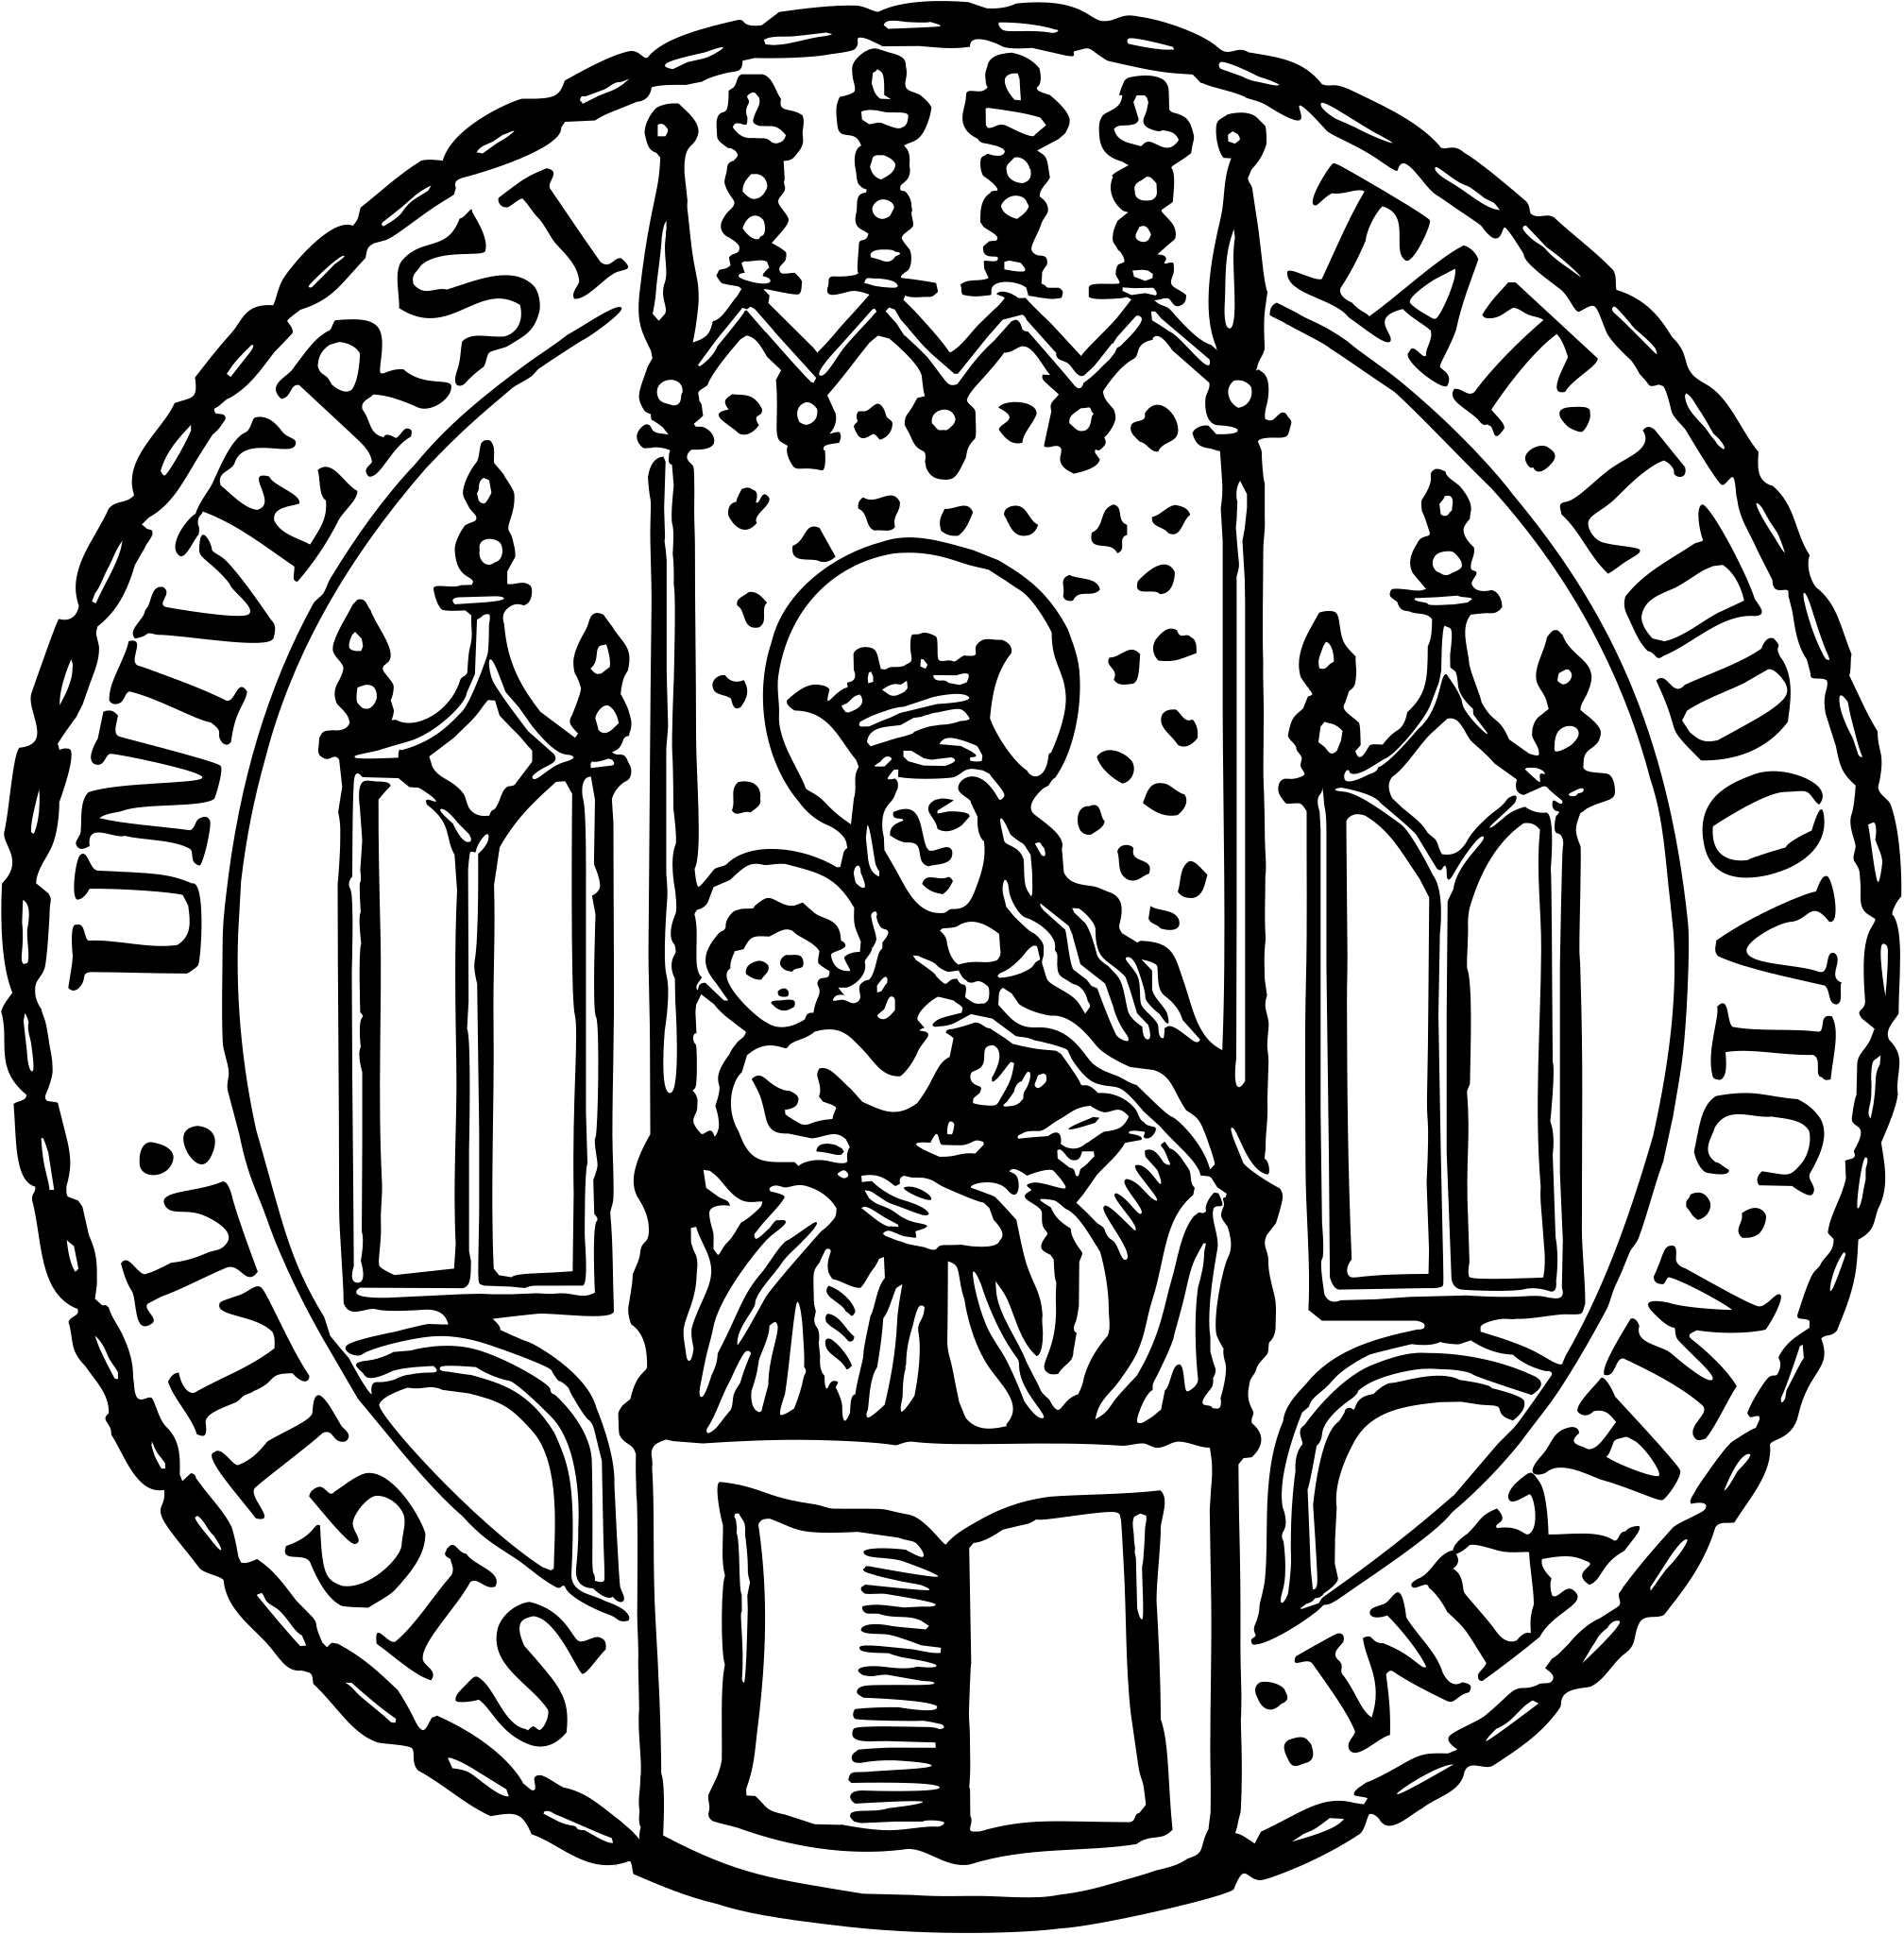
\includegraphics[width=\paperwidth, height=\paperheight, keepaspectratio]{figures/lmu-siegel.png}
%             }
%             \vfill
%         }
%     }
% }
%%%%%%%%%%%%%%%%%%%%%%%%%%%%%%%%%%%%%%

%%% COMMAND FOR PRETTY CODE HIGHLIGHTING %%%
% source: https://tex.stackexchange.com/questions/140166/making-inline-code-printing-pretty?noredirect=1&lq=1
% \newcommand\code[3][]{
%     \tikz[baseline=(s.base)]{
%         \node(s)[
%             rounded corners,
%             fill=blue!5,        % background color
%             draw=gray,          % border of box
%             %text=gray!50!black, % text color
%             inner xsep =3pt,    % horizontal space between text and border
%             inner ysep =0pt,    % vertical space between text and border
%             text height=2ex,    % height of box
%             text depth =1ex,    % depth of box
%             #1                  % other options
%         ]{\mintinline{#2}{#3}};
%     }
% }
%%%%%%%%%%%%%%%%%%%%%%%%%%%%%%%%%%%%%%%%%%%

%%% COMMAND FOR EMPTY PAGE %%%
% source: https://tex.stackexchange.com/questions/34934/add-a-new-empty-page
%\newcommand*\NewPage{\newpage\null\thispagestyle{empty}\newpage}
%%%%%%%%%%%%%%%%%%%%%%%%%%%%%%


%%%%%%%%%%%%%%%%%%%%%%
%%% PACKAGE SETUPS %%%
%%% ============== %%% 

%%% BIBLATEX SETUP %%%
% source: https://tex.stackexchange.com/questions/534565/apply-empty-style-to-the-entire-bibliography
\renewcommand{\bibsetup}{\thispagestyle{empty}}
\makeatletter
\patchcmd{\blx@endenv@bibliography}{\endlist}{\endlist\clearpage}{}{}
\makeatother
%%%%%%%%%%%%%%%%%%%%%%

%%% CLASS SETUP %%%
\setcounter{secnumdepth}{3}
\setcounter{tocdepth}{3}
%%%%%%%%%%%%%%%%%%%

%%% CSQUOTES SETUP %%%
% source: https://tex.stackexchange.com/questions/329334/quote-inline-with-italics
% \DeclareQuoteStyle[american]{english}
% {\itshape\textquotedblleft}
% [\textquotedblleft]
% {\textquotedblright}
% [0.05em]
% {\textquoteleft}
% {\textquoteright}
%%%%%%%%%%%%%%%%%%%%%%

%%% FANCYHDR SETUP %%% 
\pagestyle{fancy}
\fancyhf{}
\fancyhead[RE]{\normalfont\bfseries\sffamily\leftmark}
\fancyhead[LO]{\normalfont\bfseries\sffamily\rightmark}
\fancyhead[RO,LE]{\thepage}

\fancypagestyle{plain}{%
  %\fancyhf{}
  %\fancyhead[RO,LE]{\thepage}
}

\ChTitleVar{\bfseries\Large\rmfamily}
\ChNameVar{\Large\sffamily}

\makeatletter
\renewcommand\chaptermark[1]{%
  \markboth{%
    \ifnum \c@secnumdepth >\m@ne
      \if@mainmatter
        %\chaptername
      \fi
    \fi
    #1%
  }{}
}

\renewcommand\sectionmark[1]{\markright{\thesection\enspace #1}}
%\renewcommand\subsectionmark[1]{\markright{\thesubsection\enspace #1}}
\makeatother          
%%%%%%%%%%%%%%%%%%%%%%

%%% FONT SETUP %%%
%\renewcommand{\familydefault}{\sfdefault}
%%%%%%%%%%%%%%%%%%

%%% HYPER SETUP %%%
\hypersetup{   
    pdfpagemode = {UseNone},
    pdftitle = {\getTitleEN},
    pdfauthor = {\getAuthor},
    pdflang = {\langEN},
    colorlinks = true,     
    linkcolor = black,      
    citecolor = black,
    filecolor = black,      
    urlcolor = black       
}                        
%%%%%%%%%%%%%%%%%%%

%%% LISTINGS SETUP %%%
 % \definecolor{mygreen}{rgb}{0,0.6,0}
 % \definecolor{mygrey}{rgb}{0.8,0.8,0.8}
 % \definecolor{mymauve}{rgb}{0.58,0,0.82}

 % \lstset{ %
 %   backgroundcolor=\color{mygrey},       % choose the background color
 %   basicstyle=\ttfamily,                 % size of fonts used for the code
 %   breaklines=true,                      % automatic line breaking only at whitespace
 %   captionpos=b,                         % sets the caption-position to bottom
 %   commentstyle=\color{mygreen},         % comment style
 %   escapeinside={\%*}{*)},               % if you want to add LaTeX within your code
 %   keywordstyle=\color{blue},            % keyword style
 %   numbers=left,                         % alignment of numbers
 %   numberstyle={\small \color{black}},    % number style
 %   numbersep=9pt,                        % this defines how far the numbers are from the text
 %   stepnumber=1,
 %   stringstyle=\color{mymauve}           % string literal style
 % }
%%%%%%%%%%%%%%%%%%%%%

%%% SI SETUPS %%%
\sisetup{locale=US}                     
\sisetup{per-mode=symbol-or-fraction} 
\DeclareSIUnit \au {au}
\DeclareSIUnit \ly {ly}
\DeclareSIUnit \parsec {pc}
\DeclareSIUnit \yr {yr}
%%%%%%%%%%%%%%%%%

%%% SIDECAP SETUP %%%
% \sidecaptionvpos{figure}{t}
%%%%%%%%%%%%%%%%%%%%%

%%% TCOLORBOX SETUP %%%
% \definecolor{mygray}{rgb}{0.8,0.8,0.8}
% \tcbset{
%         on line,
%         boxsep = 2pt,
%         left = 0pt,
%         right = 0pt,
%         top = 0pt,
%         bottom = 0pt,
%         colframe = white,
%         colback = mygray
% }
%%%%%%%%%%%%%%%%%%%%%%%%

%%% TIKZ AND PGFPLOTS SETUP %%%
% \usetikzlibrary{intersections}
% \usetikzlibrary{decorations.pathreplacing, decorations.markings}
% \usetikzlibrary{tikzmark}
% \pgfplotsset{every axis/.style={scale only axis}, compat=newest}
%%%%%%%%%%%%%%%%%%%%%%%%%%%%%%%

%%% TITLESEC SETUP %%%
% source: https://tex.stackexchange.com/questions/111643/decrease-space-before-and-after-chapter-in-fncychap
\makeatletter
\patchcmd{\@makechapterhead}{\vspace*{50\p@}}{\vspace*{-20\p@}}{}{}
\patchcmd{\@makeschapterhead}{\vspace*{50\p@}}{\vspace*{-20\p@}}{}{}
\patchcmd{\DOTI}{\vskip 80\p@}{\vskip 40\p@}{}{}
\patchcmd{\DOTIS}{\vskip 40\p@}{\vskip 0\p@}{}{}
\makeatother
% \makeatletter
% \titleformat{\chapter}[frame]
%   {\normalfont}{\filright\enspace \@chapapp~\thechapter\enspace}
%   {8pt}{\LARGE\bfseries\filcenter}
% \titlespacing*{\chapter}
%   {0pt}{0pt}{20pt}
% \makeatother
%%%%%%%%%%%%%%%%%%%%%%

%%% TOC SETUP %%%
% source: https://tex.stackexchange.com/questions/5787/table-of-contents-with-page-style-empty
\AtBeginDocument{\addtocontents{toc}{\protect\thispagestyle{empty}}} 
%%%%%%%%%%%%%%%%%

% Change Chapter xy to sth else
\makeatletter
\renewcommand{\@chapapp}{Section}
\makeatother


\addbibresource{sources/bib_thesis.bib}
\allowdisplaybreaks % for pagebreaks in align environment
\begin{document}

%%%%%%%%%%%%%%%%%%%%
%%% FRONT MATTER %%%
%%% ============ %%%

\frontmatter

%%% FRONTPAGE
\begin{titlepage}   

    \vspace*{\stretch{1}}
    {\parindent0cm
    \rule{\linewidth}{.4ex}}  
  \begin{center}
    \vspace*{\stretch{0.4}}
    {\sffamily \bfseries \Huge \getTitleEN}
    \vspace*{\stretch{0.4}}
  \end{center}
    \rule{\linewidth}{.4ex}
    \vspace*{\stretch{3}}
  

  \begin{center}
    % {\rmfamily \bfseries \Large Bachelor Thesis}

    \vspace*{\stretch{0.3}}


  \begin{figure}[!h]
    \centering
    \transparent{0.2}
    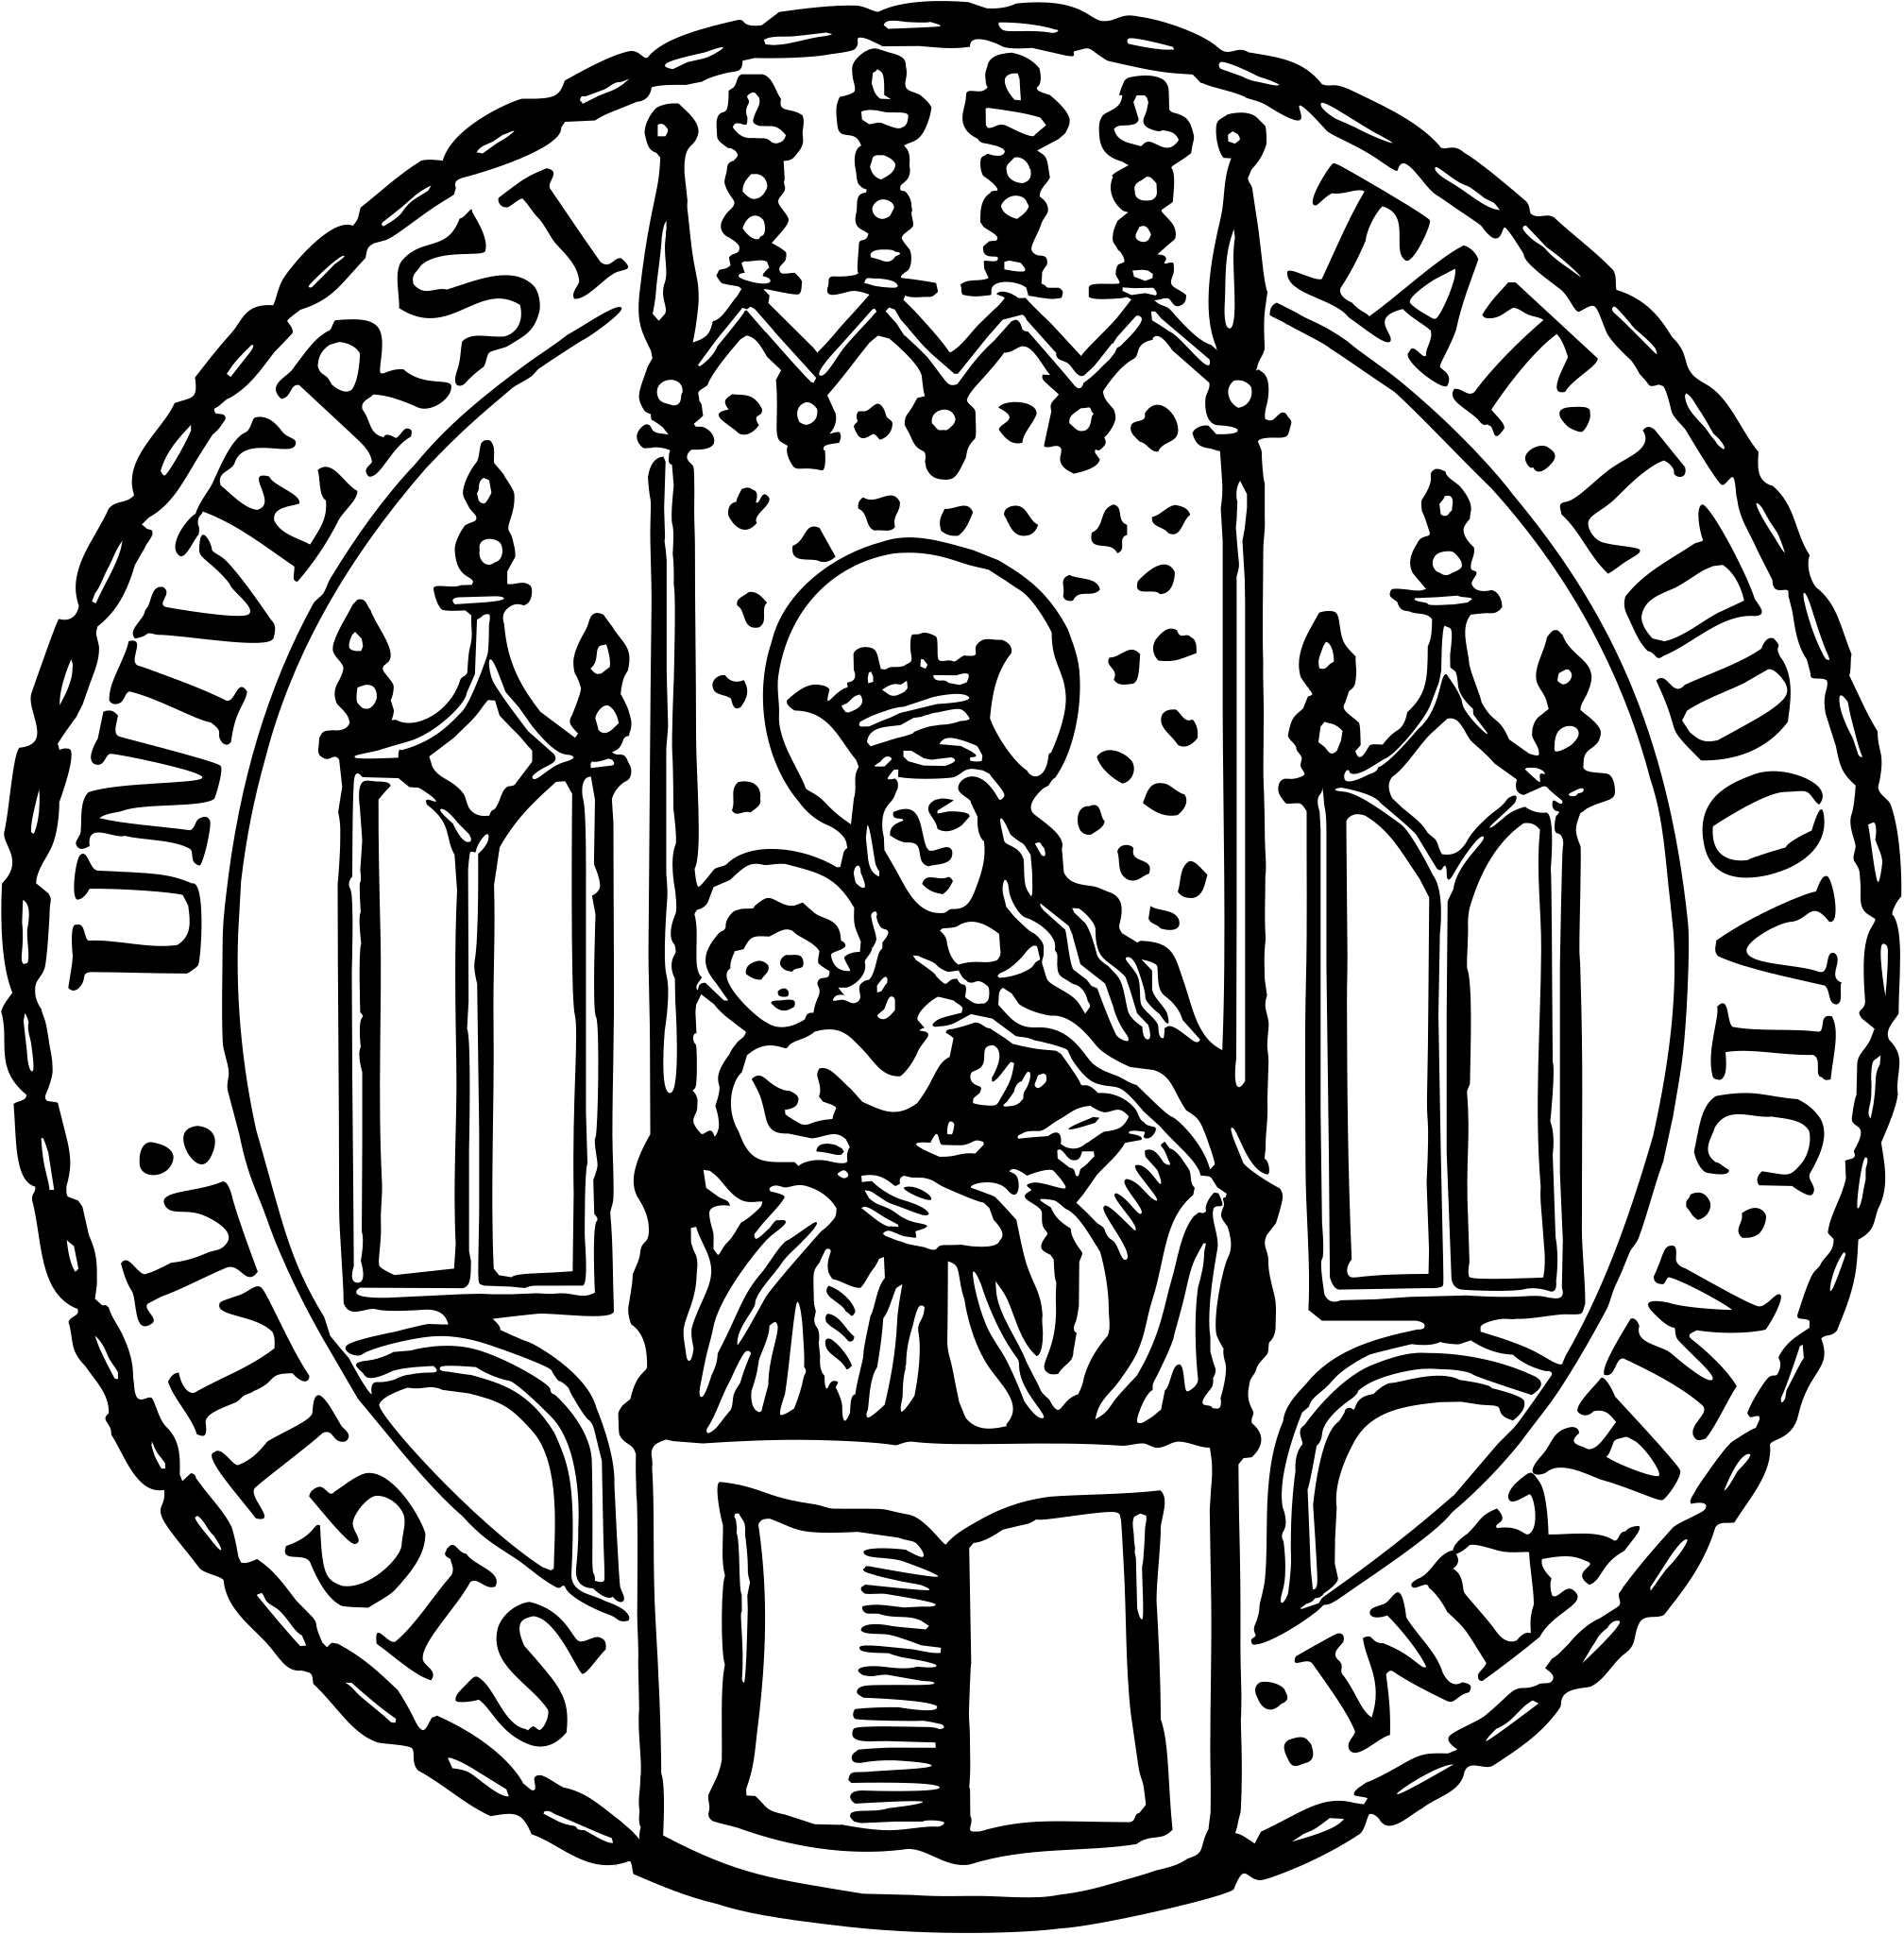
\includegraphics[scale=0.15]{figures/lmu-siegel.png}
  \end{figure}
  

    \vspace*{\stretch{2}}
     {\scshape \large
    %  University Observatory Munich \\
    %  Fakulty of Physics \\
    %  at the Ludwig-Maximilians-University \\
    %  Munich

     \vspace*{\stretch{1}}

     submitted by \\

     \vspace*{\stretch{0.3}}
     {\rmfamily \bfseries \Large \getAuthor} \\


     \vspace*{\stretch{2}}
     \getPrintLocationEN, \getSubmissionDateEN
     }
  \end{center}
  
  %\AddToShipoutPicture*{\BackgroundPic}

\end{titlepage}

\thispagestyle{empty}

\newpage\null\thispagestyle{empty}\newpage

%%% TITLEPAGE 
\begin{titlepage}   

    \vspace*{\stretch{1}}
    {\parindent0cm
    \rule{\linewidth}{.4ex}}
  \begin{center}
    \vspace*{\stretch{0.4}}
    {\sffamily \bfseries \Huge \getTitleDE}
    \vspace*{\stretch{0.4}}
  \end{center}
    \rule{\linewidth}{.4ex}
    \vspace*{\stretch{3}}


  \begin{center}
    {\rmfamily \bfseries \Large Bachelorarbeit}

    \vspace*{\stretch{0.3}}

    {\scshape \large
     Fakultät für Physik \\
     Quanten Vielteilchensysteme/ Theoretische Nanophysik\\
     Ludwig-Maximilians-Universität\\
     München
     
     \vspace*{\stretch{1}}
     
     vorgelegt von \\
    
     \vspace*{\stretch{0.3}}
     {\rmfamily \bfseries \Large \getAuthor} \\

     
     \vspace*{\stretch{2}}
     \getPrintLocationDE, \getSubmissionDateDE
     }
  \end{center}
  
\end{titlepage}

\thispagestyle{empty}
%\begin{titlepage}   

    \vspace*{\stretch{1}}
    {\parindent0cm
    \rule{\linewidth}{.4ex}}  
  \begin{center}
    \vspace*{\stretch{0.4}}
    {\sffamily \bfseries \Huge \getTitleEN}
    \vspace*{\stretch{0.4}}
  \end{center}
    \rule{\linewidth}{.4ex}
    \vspace*{\stretch{3}}
  

  \begin{center}
    {\rmfamily \bfseries \Large Bachelor Thesis}

    \vspace*{\stretch{0.3}}

    {\scshape \large
     Faculty of Physics \\
     Quantum Many-Body Systems/ Theoretical Nanophysics Group\\
     Ludwig Maximilian University\\ 
     Munich

     \vspace*{\stretch{1}}

     submitted by \\

     \vspace*{\stretch{0.3}}
     {\rmfamily \bfseries \Large \getAuthor} \\


     \vspace*{\stretch{2}}
     \getPrintLocationEN, \getSubmissionDateEN
     }
  \end{center}
  
\end{titlepage}

%\thispagestyle{empty}

%%% SUPERVISORS
\thispagestyle{empty}

\vspace*{\stretch{1}}

\begin{flushleft}
    {\large
     Supervisor:  \getSupervisorOne \\[1mm]
     %Second supervisor: \getSupervisorTwo \\
     }
\end{flushleft}

\cleardoublepage{}

\thispagestyle{empty}

%%% ACKNOWLEDGEMENT
%\chapter*{Acknowledgement}
\phantomsection\addcontentsline{toc}{chapter}{\protect Acknowledgement}
\thispagestyle{empty}

\noindent Here, you can write some acknowledgement. \\

\noindent It has been probably a hard and long way -- from your school enrollment to middle school, high school with all its ups and downs, through your time at college/university until this point of your life you have reached now. \\ 

\noindent You can be proud of yourself by all the effort, all the sweat and tears it took to graduate. \\

Do not forget that it does not only take diligence and discipline to achieve a bachelor's degree, but also luck and decent people in your life, who brought you up to this point. \\
\noindent Maybe, this is a good opportunity to thank all your colleagues, friends, teachers and family members, who were always there for you in hard and rough times.
Without people arround us that we can trust, even the most intelligent and gifted people would not have achieve any success in life. \\
\noindent Thank you!

%\thispagestyle{empty}

%%% NOTATION AND CONVENTIONS
\chapter*{Notation and Symbols}
\phantomsection\addcontentsline{toc}{chapter}{\protect Notation and conventions}
\begin{tabular}{cp{0.9\textwidth}}
  $\lambda$ & flow parameter; in the literature sometimes also denoted by $B$ \\
  $\hat\cdot$ & denotes that $\cdot$ is an operator which does not commute with every other operator\\
  $1$ & indicates $1\in\N$ or the identity operator $\hat{\1}\eqdef \1$\\
  $\NO \hat A\NO$ & normal ordering of operator $\hat A$\\ 
  $\CR_k$ & $k^\mathrm{th}$ bosonic creation operator \\
  $\AN_k$ & $k^\mathrm{th}$ bosonic annihilation operator \\
  $[\hat{ A},\hat{ B}]$ & commutator of operators $\hat{ A},\hat{ B}$ \\
  $\hat A^\dagger$ & adjoint of an operator $\hat{ A}$ \\
  $z^*$ & complex conjugate of $z\in\C$ \\
  $\delta_{\alpha,\beta}$ & Kronecker-Delta of $\alpha,\beta$ \\ 
  $\partial_x$ & partial derivative $\frac{\partial}{\partial x}$ w.r.t. $x$\\
  $\overset{\CircledTop{2}}{=}$ & Equality up to second order, i.e. higher order terms are neglected.\\
  $\hbar=1$ & reduced Planck's constant is set to $1$\\
  $+\mathrm{h.c.}$ & plus the Hermitian conjugate of the previous term\\
  $\sim$ & approximately proportional to\\
  $\underline{\underline E}_N$ & $N\times N$ identity matrix
\end{tabular}\\
%\vspace{2cm}
%For convenience, the most important constants used in the Thesis are listed here:








\thispagestyle{empty}

%%% ABSTRACT
%\chapter*{Abstract}
\phantomsection\addcontentsline{toc}{chapter}{\protect Abstract}
\thispagestyle{empty}

Here you can write a summary, what your thesis is about or short introduction to your thesis.

\bt

%\thispagestyle{empty}

%%% TABLE OF CONTENT
\pdfbookmark{\contentsname}{Contents}
\tableofcontents 
\clearpage
\thispagestyle{empty}

%%% LIST OF FIGURES
\cleardoublepage
% \phantomsection
\addcontentsline{toc}{chapter}{\listfigurename}
\listoffigures



%%%%%%%%%%%%%%%%%%%%
%%% MAIN MATTER %%%%
%%% =========== %%%%

\mainmatter

%%% INTRODUCTION 
\chapter{Introduction}
The flow equation approach was independently discovered by Franz Wegner \cite{https://doi.org/10.1002/andp.19945060203} and by Stanislaw D. Glazek and Kenneth G. Wilson \cite{PhysRevD.48.5863} as a new renormalization technique to diagonalize, or at least block-diagonalize, Hamiltonians. It is also known under the names Continuous Unitary Transformation (CUT), Double Bracket Flow, or Isospectral Flow, and has been successfully applied to a variety of physical systems, including the Kondo model, interacting bosons, and electron-phonon interaction \cite{Wegner_2006}.\par
This thesis deals with the application of the flow equation method to quadratic bosonic Hamiltonians. Two cases are distinguished: In the first case the Hamiltonian is purely quadratic, in the second case the Hamiltonian still has the same basic structure, but now the coefficients depend on (bosonic) occupation numbers.\\
The first case occurs, for example, in the BEC polaron problem at infinite impurity mass. The dependence on occupation numbers comes into play when this impurity is not fixed, that is, when it has a finite mass.\par
%, or in the study of magnons in doped antiferromagnets.\par
This thesis is organized as follows: First, we will provide a brief introduction to the flow equation approach and elaborate on some of the problems it entails in section \ref{Theoretical Background}. We will also give an overview on the Bose Polaron problem by discussing the Fröhlich Hamiltonian and the Lee-Low-Pine (LLP) Transformation. The flow equations  both for the purely quadratic case and the case where the coefficients depend on the bosonic occupation numbers will formulated in section \ref{Determining the Flow Equations}. This section will be supplemented by detailed calculations in appendix \ref{Detailed Calculations}\\
The flow equations for the purely quadratic case will be tested on a one dimensional Bose polaron model in section \ref{Results} and compared to the findings of Grusdt \emph{et al.}\cite{Grusdt_2017}. \\
We then close with a conclusion and an outlook in section \ref{Conclusion and Outlook}.

%%% CHAPTER 02
\chapter{Theoretical Background}\label{Theoretical Background}
\section{The Flow Equation Approach}
In this section we introduce the mechanism and general idea behind the flow equation approach. Then we will axiomatically define normal ordering for its relevance to our subsequent discussion about truncation schemes. \\
After that, we will give a brief overview of the Bose polaron problem. The Hamiltonian which will be introduced there can be brought into the purely quadratic form required for our flow equations derived in Section \ref{Determining the Flow Equations} by a Lee-Low-Pines transformation, an introduction to which will be given at the end of this section. %. This is why we close this section by sketching the idea behind the Lee-Low-Pines transformation.
\subsection{General Mechanism}\label{General Mechanism}
Since this section is intended to be a concise and rather operational overview on the flow equation approach, we refer to S. Kehrein's in-depth and very pedagogical introduction for further reading \cite{kehrein2006flow}. This is also the textbook on which this section is based on, unless indicated otherwise.\par 
Our starting point will be some Hamiltonian $\ham$ and our goal will be to continuously transform $\ham$ into an unitarily equivalent diagonal Hamiltonian. This sequence of transformations $\hat U$ is ordered by a flow parameter $\lambda$ with $\left[\lambda\right]=\mathrm{Energy}^{-2}$ and will be chosen such that the off-diagonal elements in  
\begin{equation}\label{FEQ_U_def}
\ham(\lambda)=\hat U(\lambda)\ham (\lambda = 0)\hat U^\dagger (\lambda)
\end{equation}
vanish in the limit $\lambda\rightarrow\infty$. $\hat U(\lambda)$ is connected to $\hat\eta(\lambda)$ by
\begin{equation}
\hat\eta(\lambda)\defeq\frac{\mathrm d\hat U(\lambda)}{\mathrm d\lambda}\hat U^\dagger(\lambda)=-\hat\eta^\dagger(\lambda)%\defeq\hat\eta
\end{equation}
%Stone's theorem on one-parameter unitary groups \cite{doi:10.1073/pnas.16.2.172} guarantees the existence of $\hat \eta(\lambda)$ which is anti-hermitian, i.e. $\hat\eta(\lambda) = -\hat\eta^\dagger(\lambda)$, and fulfills 
%\begin{equation}
%\hat U(\lambda) = e^{\hat\eta(\lambda)}.
%\end{equation} 
where $\hat\eta(\lambda)$ is called the antihermitian generator of the unitary transformation $\hat U(\lambda)$ or simply the generator of the flow. Applying the Baker-Campbell-Hausdorff formula to equation \ref{FEQ_U_def}, or simply differentiating both sides of equation \ref{FEQ_U_def} with respect to $\lambda$, yields
\begin{equation}\label{FEQ_ODE_def}
\frac{\mathrm d\ham(\lambda)}{\mathrm d\lambda} = \left[\hat\eta(\lambda),\ham(\lambda)\right].
\end{equation}
This differential equation is what we will refer to as the flow equation for the Hamiltonian $\ham (\lambda)$. 
The explicit computation of the unitary transformation from the generator of the transformation is generally complicated and usually not of interest because it is not required for finding the diagonal Hamiltonian. It involves the $\lambda$-ordering operator 
\begin{equation}
\hat T_\lambda\left(\hat\eta(\lambda_1)\ldots\hat\eta(\lambda_n)\right)\defeq\hat\eta(\max\limits_{i=1,\ldots,n}\lambda_i)\ldots\hat\eta(\min\limits_{i=1,\ldots,n}\lambda_i)
\end{equation}
which commutes generators with larger flow parameters further to the left.
Then the unitary transformation is given by
\begin{align}
\hat U(\lambda)&=\hat T_\lambda\exp\left(\int_0^\lambda\mathrm d\lambda^\prime \hat\eta(\lambda^\prime)\right)\\
&=1+\Sum_{n=1}^\infty \frac1{n!}\int_0^\lambda\mathrm d\lambda_1\ldots\mathrm d\lambda_n\hat T_\lambda\left(\hat\eta(\lambda_1)\ldots\hat\eta(\lambda_n)\right).
\end{align}
From now on, the $\lambda-$dependence of $\hat\eta,\ham$ and $\hat U$ will usually be notationally dropped. \\
For every $\hat U$ there exists one and only one $\hat\eta$ which generates the unitary transformation defined by $\hat U$. However, there may be several $\hat U$ which let $\ham(\lambda = 0)\eqdef \ham^{(0)}$ flow to (the evidently unique) diagonal Hamiltonian $\ham(\lambda=\infty)\eqdef \ham^{(\infty)}$ so in general there is more than one good choice for $\hat\eta$. \\
It turns out that in most cases setting
\begin{equation}\label{FEQ_eta_def}
\hat\eta = \left[\ham_{\mathrm{diag.}},\ham \right],
\end{equation}
where $\ham_{\mathrm{diag.}}$ is the diagonal part of the Hamiltonian, achieves the desired diagonalization.  \par
We are often in a situation where a given system described by $\ham_0$ with known eigenenergies  and eigenstates is well understood if certain interaction terms $\ham_{\mathrm{int}}$ are omitted. In this case, we can write $\ham = \ham_0 + \ham_{\mathrm{int}}$ and thus
\begin{equation}\label{FEQ_can_eta_def}
\hat\eta = \left[\ham_0, \ham_{\mathrm{int}}\right].
\end{equation}
This choice for $\hat \eta$ is called the canonical generator and is also the choice for the generator that will be adopted in this thesis.. \\
A good benchmark that indicates how diagonal the interaction Hamiltonian is at a given point in the flow, is to check if the the trace of its square becomes smaller in the flow:
\begin{equation}\label{check_trace}
\frac{\mathrm d}{\mathrm d \lambda}\mathrm{Tr}\left(\ham^2_{\mathrm{int}}\right)\leq 0
\end{equation}
It can be proved \cite[pp. 27-28]{kehrein2006flow} that this is always the case iff 
\begin{align}\label{useless_check}
\mathrm{Tr}\left(\ham_0\ham_{\mathrm{int}}\right)=\mathrm{Tr}\left(\frac{\mathrm d\ham_0}{\mathrm d\lambda} \ham_{\mathrm{int}}\right)=0
\end{align}
Note, however, that a complete diagonalization of the Hamiltonian may not always be worthwhile, since for practically relevant Hamiltonians one almost always has to introduce approximations in order to obtain closed-form flow equations \cite{Wegner_2006}. Thus, in some cases, one might want to perform only weak unitary transformations, making the flow converge only to a block diagonal form \cite{Wegner_2006}. \\
In this thesis we will construct the flow so that it in fact flows to a diagonal Hamiltonian, but it is still good to keep in mind that the flow equation approach can be useful even if it is only used to transform the Hamiltonian into a block diagonal form that may be easier to diagonalize by other methods such as block-wise exact diagonalization.\\ 
In the following section, we will introduce normal ordering - an important concept for controlling the error in the aforementioned often-needed approximations.
\subsection{Normal Ordering}
Normal ordering plays an essential role in successfully applying to flow equation approach to realistic Hamiltonians. In our definition of normal ordering, we closely follow \cite[pp. 62-63]{kehrein2006flow} which in turn is based upon unpublished notes by F. Wegner.\\
Let $\hat\alpha_k\in\{\AN_k,\CR_k\}$ and consider some normalized reference state $|\psi_{NO}\rangle$. Moreover, we define the contractions 
\begin{equation}\label{contractions_def}
C_{k,l}\defeq \langle \psi_{NO}|\hat\alpha_k\hat\alpha_l|\psi_{NO}\rangle.
\end{equation}
Then it follows that
\begin{equation}
\left[\hat\alpha_k,\hat\alpha_l\right] = C_{k,l}-C_{l,k}
\end{equation}
which can be proved readily by applying the canonical commutation relations to equation \ref{contractions_def} and by using the normalization of $|\psi_{NO}\rangle$.
The normal ordering of an operator $\hat O$ composed of creation and annihilation operators is defined by the following three rules:
\begin{enumerate}
\item c-numbers are unaffected by normal ordering:
\begin{equation}
\NO 1\NO = 1
\end{equation}
\item Linearity:
\begin{equation}
\NO c\ \hat O_1+\hat O_2\NO = c \NO \hat O_1\NO+\NO \hat O_2\NO\ \forall c\in\C
\end{equation}
\item Recurrence relation:
\begin{equation}\label{recurrence relation}
\hat\alpha_k\NO\hat O\NO=\NO\hat\alpha_k\hat O\NO + \Sum_l C_{k,l}\NO{\partial_{\hat\alpha_l}\hat O}\NO 
\end{equation}
The derivative is performed symbolically w.r.t. $\hat\alpha_l$.
\end{enumerate}
An important property of normal ordered operators is that within an normal ordered expression, products of operators can be permuted arbitrarily.\\
Furthermore, when the normal ordering is performed with respect to the vacuum, normal ordering an operator is equivalent to successively commuting all creation operators to the left and all annihilation operators to the right. 
\subsection{Truncation Schemes}\label{Truncation Schemes}
The crux of the flow equation approach lies in the fact that for many Hamiltonians, the flow creates higher and higher interaction terms. To illustrate this, consider a Hamiltonian which can be split into a quadratic $\ham_0$ and a quartic $\ham_{\mathrm{int}}$, i.e. they contain terms with two respectively four creation or annihilation operators. \\
Evaluating the commutator \ref{FEQ_can_eta_def} yields a generator which is still of the same structure as the original Hamiltonian. However, evaluating equation \ref{FEQ_ODE_def}  yields fourth order terms from the commutators of quadratic and quartic terms and sixth order terms from the commutators of quartic and quartic terms. This might suggest that the flow Hamiltonian is of order six, but then also the commutators of these sixth order terms with the canonical generator with terms up to quartic order have to be considered, which in turn creates terms of order eight and so forth. \par
It follows that, for practical purposes, this sequence must be truncated at some point. Normal ordering can be thought of as a procedure to organize the higher order terms generated in the flow, because the normal ordered expression consisting of all quadratic creation or annihilation operator terms contains all the information about the particle energies, and the normal ordered expression consisting of all quartic creation or annihilation operator terms contains all the information about the two-particle interaction and so on \cite{kehrein2006flow}. Without normal ordering, for example, fourth-order terms might also contribute to one-particle energies. Thus, a normally ordered expression organizes its terms by the order of their interaction. Since higher order interactions generally contribute less than lower order interactions, this is the correct way to truncate a sequence. \par
With respect to which state the Hamiltonian should be normal ordered, i.e. with respect to which state the contractions \ref{contractions_def} should be defined, is subtle. It should be defined with respect to the ground state $|GS\rangle$ of the diagonal Hamiltonian $\ham^{(\infty)}$, because we want the interaction terms to be ordered by their interaction order in our actual physical system. But there are two problems with this: First, the ground state of the diagonal Hamiltonian is not necessarily known; second, this state changes because the basis changes at each step of the flow, i.e. 
\begin{equation}
|GS(\lambda)\rangle = \hat U(\lambda)\hat U^\dagger(\lambda=\infty)|GS\rangle.
\end{equation}
Intuitively, this is clear: We first let the flow run backwards from $\lambda=\infty$ to $\lambda = 0$ and then let $|GS(\lambda=0)\rangle$ flow until $|GS(\lambda)\rangle$ which is the correct ground state in the basis of a given point $\lambda$ in the flow.\\
A possible solution to our two problems is to first start with normal ordering w.r.t. some arbitrary state (e.g. the vacuum) to get a first guess for the ground state of the diagonal Hamiltonian and to iteratively improve that guess by repeatedly traversing the flow. \par
Although this method has not found widespread adoption when using the flow equation approach because the error induced by a \grqq na\"ive\grqq\  normal ordering prescription is usually not large \cite{kehrein2006flow}, and it may sometimes be easier just to consider more terms in the flow instead of working with the correct normal ordering prescription, it is important not to forget that not all normal ordered expansions and truncation schemes are equally well-behaved and can introduce differently sized errors.

\section{The Bose Polaron Problem}
\subsection{(Beyond) The Fröhlich Hamiltonian}\label{(Beyond) The Fröhlich Hamiltonian}
The Fröhlich Hamiltonian is a model Hamiltonian that describes the interaction between a single quantum particle and a phonon reservoir, such as a crystal lattice.% or a Bose-Einstein condensate (BEC) \cite{Grusdt_2017}. 
It was introduced by Herbert Fröhlich in 1954 to study the effect of electron-phonon coupling on the electrical conductivity of polar crystals \cite{doi:10.1080/00018735400101213} but can also be used to describe the interaction of an impurity with the Bogoliubov phonons of an BEC \cite{Myśliwy2020}.% or an lattice of atoms  
This interaction leads to the formation of a quasiparticle called the Bose polaron because the impurity atom becomes \grqq dressed\grqq\ in a cloud of phonons, which changes important properties of the impurity, such as its effective mass and mobility \cite{Grusdt_2017}.\\ 
We follow Grusdt \emph{et al.} \cite{Grusdt_2017} and write the Fröhlich Hamiltonian in one dimension in the following form:
\begin{equation}\label{Fröhlich}
\ham_F = g_{IB}n_0+\frac{\hat p^2}{2M}+\int\mathrm d k\omega_{ k}\CR_{ k}\AN_{ k}+\sqrt{\frac{n_0}{2\pi}}g_{IB}\int\mathrm d k W_k e^{ik\hat x}\left(\AN_{ k}+\CR_{- k}\right)
\end{equation}
Here $g_{IB}$ is the boson-impurity coupling constant which characterizes the strength of their interaction and $n_0$ is the density of the Bose gas. The second term describes the kinetic energy of the impurity of mass $M$ in first quantized form. The third term accounts for the energy of the Bogoliubov phonons with the Bogoliubov dispersion given by 
\begin{equation}\label{bog_disp}
w_k=ck\sqrt{1+\frac12\xi^2k^2}
\end{equation}
where we introduced $\xi$ as the healing length %of the Bose condensate 
and $c$ as the speed of sound. % in the condensate. 
The last term describes interactions between the impurity and the phonons. It can be thought of modeling a process where a phonon in mode $k$ is first absorbed and then reemitted as a phonon in mode $-k$ with an appropriate change in both amplitude and phase. For this process, the scattering amplitude is
\begin{equation}\label{W_k_def}
W_k = \left(\frac{(\xi k)^2}{2+(\xi k)^2}\right)^{1/4}
\end{equation}
and the change in phase depends on the position operator of the impurity (again in first quantization).\par
It has been shown that in order to accurately describe the effective mass of Bose polarons, the Fröhlich Hamiltonian alone does not suffice and two-phonon scattering terms have to be included in the Hamiltonian \cite{Grusdt_2017}. Then the full Hamiltonian reads
\begin{equation}\label{full_ham}
\ham = \ham_F + \ham_{2\mathrm{ph}}.
\end{equation}
It should be noted at this point that a 1D model is not only interesting from a theoretical perspective, since experimental setups in one dimension are possible and have successfully been realized \cite{Catani}. The inclusion of two-phonon scattering terms leads to very good agreement of experiment and theory when the coupling between the impurity and the phonons is not too strong \cite{Grusdt_2017}. \\
The aforementioned two-phonon scattering terms are quadratic and are again proportional to the boson-impurity coupling constant \cite{Grusdt_2017, PracticalTraining}:
\begin{equation}
\ham_{2\mathrm{ph}}=\frac{g_{IB}}{2\pi}\int\mathrm d k\mathrm d k^\prime \left(c_k\CR_k-s_k\AN_{-k}\right)\left(c_{k^\prime}\AN_{k^\prime}-s_{k^\prime}\CR_{-k^\prime}\right)e^{i(k-k^\prime)x}
\end{equation}
The coefficients $c_k$ and $s_k$ can be obtained from 
\begin{subequations}
\begin{align}
W_k &= c_k - s_k\\
W_k^{-1} &= c_k + s_k
\end{align}
\end{subequations}
In principle, additional interactions between the Bogoliubov phonons have to be accounted for. However, those only become relevant when the boson-boson interaction constant $g_{BB}$ becomes large, the density $n_0$ becomes small or, equivalently, the coupling strength \begin{equation}\gamma\defeq\frac{m_B g_{BB}}{n_0}\end{equation} is large. Because this regime will not be considered in this thesis, $\ham_F$ and $\ham_{2\mathrm{ph}}$ model the polaron problem well for our purposes.\\
For future reference, we will now also introduce the 1D boson–boson s-wave scattering length 
\begin{equation}
a_{BB}=-\frac{2}{m_Bg_{BB}}
\end{equation}
where \begin{equation}m_B = \frac{1}{\sqrt{2c\xi}}\end{equation} is the mass of the bosons
and the dimensionless parameter 
\begin{equation}
\eta\defeq \frac{g_{IB}}{g_{BB}}
\end{equation}
to quantify how the interaction strength between impurity and boson compares to the strength of the boson-boson interactions.
%In paramter regime we are interested in, 
%For small $\eta$, the Fröhlich Hamiltonian describes the physics of the impurity accurately. For strong coupling, however, two-phonon terms must be included and our full Hamiltonian reads

\subsection{The Lee-Low-Pines (LLP) Transformation}
The Lee-Low-Pines (LLP) transformation \cite{LLP} dramatically simplifies solving the full Hamiltonian \ref{full_ham}. By making use of the fact that the total system momentum is conserved (which follows from the translational invariance of $\ham$) it allows us to transform to a reference frame co-moving to the impurity with the impurity in its center. \\
Let $\hat p$ be the momentum operator of the impurity and \begin{equation}\hat p_b= \int\mathrm d k k \CR_k\AN_k\end{equation} be the momentum operator of the bosons. 
We take advantage of the fact that the total system momentum operator is
\begin{equation}
\hat P_{\mathrm{tot}} = \hat p_b + \hat p.
\end{equation}
and then define
\begin{equation}
\hat U_{\mathrm{LLP}}\defeq \exp\left(i\hat x\cdot \hat p_b\right)
\end{equation}
Intuitively, it is clear why this performs the desired transformation: $\hat p_b$ is the generator of translations for the bosons and therefore $\hat U_{\mathrm{LLP}}$ translates all bosons by the (correct) amount $\hat x$, which is the position operator of the impurity. On the other hand, $\hat x$ generates translations in momentum space for the impurity and therefore $\hat U_{\mathrm{LLP}}$ shifts the impurity momentum by the boson momentum. \\
Hence, upon applying the transformation, we have indeed transformed into a frame co-moving with the impurity where the impurity is in the center.\\
Lee, Low and Pines \cite[eq. (8)]{LLP} then went on to show that
\begin{subequations}
\begin{align}
\hat U_{\mathrm{LLP}}^\dagger \hat p \hat U_{\mathrm{LLP}} &= \hat p -\hat p_b\\
\hat U_{\mathrm{LLP}}^\dagger \AN_k \hat U_{\mathrm{LLP}} &= \AN e^{i k\hat x}.
\end{align}
\end{subequations}
%This is the desired transformation because $\hat p$ is the generator of (infinitesimal) translations of the impurity and $\hat x$ generates translations of the impurity in momentum space.\\
Therefore the Hamiltonian under the LLP transformation reads:
\begin{align}\label{ham_LLP}
\hat U_{\mathrm{LLP}}^\dagger\ham\hat U_{\mathrm{LLP}} &\defeq \ham_{\mathrm{LLP}}(p) =g_{IB}n_0+\frac{1}{2M}\left(p-\int\mathrm d k k \CR_k\AN_k \right)^2+\int\mathrm d k\omega_{ k}\CR_{ k}\AN_{ k}\\
&+\sqrt{\frac{n_0}{2\pi}}g_{IB}\int \mathrm d k W_k \left(\AN_{ k}+\CR_{- k}\right) + \frac{g_{IB}}{2\pi}\int\mathrm d k\mathrm d k^\prime \left(c_k\CR_k-s_k\AN_{-k}\right)\left(c_{k^\prime}\AN_{k^\prime}-s_{k^\prime}\CR_{-k^\prime}\right)\nonumber
\end{align}
In the new frame the impurity momentum is a constant of motion because in the original frame the total momentum was a constant of motion. This allows us to replace the impurity momentum with the $c$-number $p$ in the Hamiltonian \ref{ham_LLP} which will be referred to as LLP-Hamiltonian.




%%% CHAPTER 03
\chapter{Deriving the Flow Equations}\label{Determining the Flow Equations}
This section explains how the flow equations can be derived. For detailed calculations, please refer to the Appendix \ref{Detailed Calculations}.\\
First, we will consider the purely quadratic case without $\hat n$-dependencies and discuss how the flow equations can be applied to the Bose polaron problem in the heavy impurity limit. Then a possible exact diagonalization procedure will be explained, as it will serve as our benchmark for the flow equations in Section \ref{Results}.\\
Second, we will consider the case with $\hat n$-dependence, such as the LLP-Hamiltonian with finite impurity mass. Again, we will only sketch the steps necessary to arrive at the flow equations while the full calculations can be found in the Appendix \ref{feq_ndep_section}. These equations will not be put to the test in the scope of this thesis, but we will try to assess the prospects of successfully applying them to the LLP-Hamiltonian at the end of this section.
\section{Purely Quadratic Case}
\subsection{Applying the Formalism}
In the purely quadratic case where the coefficients do not depend on the occupation numbers and where a static impurity is considered, exact flow equations \ref{feq_won_I}-\ref{feq_won_IV} can be derived. In particular, the flow Hamiltonian $\ham(\lambda)$ is of the same quadratic form as the original Hamiltonian
\begin{equation}\label{def_purely_quadratic_hamiltonian}
\ham \defeq \ham_0+\ham_{\mathrm{int}} \defeq \Sum_k \omega_k \CR_k\AN_k+\Sum_{q\neq q^\prime}V_{q,q^\prime}\CR_q\AN_{q^\prime}+\Sum_{p,p^\prime}\left(W_{p,p^\prime}\CR_p\CR_{p^\prime}+\mathrm{h.c.}\right)
\end{equation}
 and no truncation scheme as discussed in Section \ref{Truncation Schemes} has to be employed. For details on the calculations, see Section \ref{Deriving the Flow Equations in the Case of No n-Dependence}.\par 
We followed precisely the recipe introduced in Section \ref{General Mechanism}: First the canonical generator \ref{FEQ_eta_def} is evaluated (see equation \ref{eta_wo_n_final}). Then the derivative of the flow Hamiltonian is determined by the commutator of the generator and the Hamiltonian in equation \ref{FEQ_ODE_def}. The relevant terms \ref{wo_n_I}-\ref{wo_n_IV} are evaluated separately by only making use of the bosonic commutation relations. The flow equations then follow by a simple comparison of coefficients from the quadratic (plus a constant energy $\epsilon$) ansatz for the flow Hamiltonian.\par
Note that the resulting flow equations \ref{feq_won_I}-\ref{feq_won_IV} suggest that they are exact in the sense that if the flow is completely traversed, the flow Hamiltonian will be exactly diagonal because in first order
\begin{subequations}
\begin{align}
V_{q,q^\prime}&\sim \exp\left(-(\omega_q-\omega_{q^\prime})^2\right)\xlongrightarrow{\lambda\rightarrow\infty}0\\
W_{p,p^\prime}&\sim \exp\left(-(\omega_p+\omega_{p^\prime})^2\right)\xlongrightarrow{\lambda\rightarrow\infty}0,
\end{align}
\end{subequations}
assuming that there are no degeneracies. If there were, it would mean that  $(\omega_q-\omega_{q^\prime})^2=0$ for some pair $q,q^\prime$ and that the corresponding matrix element $V_{q,q^\prime}$ is not exponentially suppressed in first order of the flow equations. Alternatively, near-degeneracies may render the convergence so slow that the corresponding matrix elements decay so slowly that the flow would have to be traversed an unreasonable or impractical distance to achieve sufficient suppression.  Fortunately, the flow equations \emph{can} still be successful in some cases \cite{PhysRevD.49.4214} because the second order terms (terms that come from the commutator of $\hat\eta$ and $\ham_{\mathrm{int}}$) coupling the ODEs for the different matrix elements are non-trivial and might, depending on the initial condition, even sufficiently suppress degenerate matrix elements.
It follows that applying the equations to a concrete problem provides the best test of their performance and convergence properties.\\
Also, checking the condition \ref{check_trace} is indeed a strong indicator for good convergence properties but does not necessarily imply that all elements in $\ham_{\mathrm{int}}$ converge to 0 when degeneracies are present, which is why we do not explicitly evaluate of the conditions \ref{useless_check} that in turn imply \ref{check_trace}.
\subsection{Application to the 1D Bose Polaron Model}
In the heavy impurity limit $M\rightarrow \infty$, the dependence of the occupation numbers in the LLP-Hamiltonian \ref{ham_LLP} vanishes and we get an Hamiltonian which differs from the purely quadratic form we discussed in the last section only by linear terms. Before we discuss the significance of these linear term we will address the fact that the integrals in there have to discretized for numerical treatment.\\
To this end, we will restrict ourselves to a discrete number of modes $k$ where $0<\Lambda_{IR}\leq |k|\leq\Lambda_{UV}<\infty$ . $\Lambda_{IR}$ denotes the infrared and $\Lambda_{UV}$ denotes the ultraviolet cut-off. We will work with values $\Lambda_{IR}\xi= 10^{-1}$ and $\Lambda_{UV}\xi= 10^1$ because this range includes phonons with momenta $k\sim1/\xi$ which are critical for defining essential properties of the Bose polaron \cite{Grusdt_2017}. \\
Of course, considering a larger number of $k$ values is generally better, but involves significant computational cost. That is why the spacing $\Delta k=\frac{2\pi}{L}$ (where $L$ is a constant which describes the size of the system) between two adjacent $k$ values will be not be chosen too small. Reasonable values are of order $\Delta k\sim 10^{-1}\xi$.  \\
These values are small enough that we are allowed to approximate integrals by sums
\begin{equation}
\int\mathrm d k\rightarrow \Delta k\Sum_k
\end{equation}
ranging over a discrete and finite grid of size $N\in\N$.
The commutation relations of the creation and annihilation operators in $\ham_{\mathrm{LLP}}$ are $\left[\AN_k,\CR_{k^\prime}\right]=\delta(k-k^\prime)$. Our new discrete operators will obey the same commutation relation with a Kronecker-delta instead of the Dirac-delta.
The transition from the continuous to the discrete case is done by coarsening the annihilation and creation operators
\begin{equation}
\AN_k^{\left(\dagger\right)}\rightarrow \frac1{\sqrt{\Delta k}}\AN_k^{\left(\dagger\right)}
\end{equation}
(see \cite[eq. (7)]{PracticalTraining})
and the LLP-Hamiltonian becomes:
\begin{align}\label{ham_LLP_discrete}
\ham_{\mathrm{LLP}}^{\mathrm{discr.}} &=g_{IB}n_0+\Sum_k \omega_{ k}\CR_{ k}\AN_{ k}+\sqrt{\frac{n_0\Delta k}{2\pi}}g_{IB}\Sum_k W_k \left(\AN_{ k}+\CR_{- k}\right) \\ &+ \frac{g_{IB}\Delta k}{2\pi}\Sum_{k,k^\prime} \left(c_k\CR_k-s_k\AN_{-k}\right)\left(c_{k^\prime}\AN_{k^\prime}-s_{k^\prime}\CR_{-k^\prime}\right)\nonumber
\end{align}
It would be conceivable to extend our flow equations to allow for linear terms in our Hamiltonian. In this case, it would again be possible to obtain a closed set of flow equations. \\
However, this can be avoided because the linear terms  $W_k \left(\AN_{ k}+\CR_{- k}\right)$ can be eliminated by applying the displacement operator 
\begin{equation}
\hat D(\underline\alpha)\defeq\exp\left(\sum_k\alpha_k\CR_k-\mathrm{h.c.}\right)=\exp\left(-\underline\alpha^\dagger{\underline{\underline\Omega}}\ \underline{\hat a}\right)
\end{equation}
to the discrete LLP-Hamiltonian \cite{PracticalTraining}. Here we introduced the symplectic $2N\times2N$ matrix
\begin{equation}\label{symplectic_matrix}
{\underline{\underline\Omega}}=\begin{pmatrix}\underline{\underline E}_N & 0\\ 0 & -\underline{\underline E}_N\end{pmatrix}
\end{equation}
and the notation
\begin{equation}\label{cr_an_vector}
\underline{\hat a} = \left(\AN_{k_1},...,\AN_{k_N},\CR_{k_1},...,\CR_{k_N}\right)^T
\end{equation}
for vectors of creation and annihilation operators as well as
\begin{equation}\label{c-number_vector}
\underline\alpha = \left(\alpha_{k_1},...,\alpha_{k_N},\alpha_{k_1}^*,...,\alpha_{k_N}^*\right)^T\in\C^{2N}
\end{equation}
for vectors of c-numbers. \par %In this context $N$ is equal to the number of modes on our discrete grid.\par
The displacement operator shifts creation and annihilation operators by a given c-number:
\begin{subequations}
\begin{align}
\hat D^\dagger(\underline \alpha)\AN_{k_i}\hat D(\underline\alpha)&=\AN_{k_i}+\alpha_{k_i}\\
\hat D^\dagger(\underline \alpha)\CR_{k_i}\hat D(\underline\alpha)&=\CR_{k_i}+\alpha_{k_i}^*
\end{align}
\end{subequations}
This can be proved readily with the help of the Baker-Campbell-Hausdorff formula.
Simliarly, one can convince oneself that
\begin{subequations}
\begin{align}
\hat D(\underline \alpha)\AN_{k_i}\hat D^\dagger(\underline\alpha)&=\AN_{k_i}-\alpha_{k_i}\\
\hat D(\underline \alpha)\CR_{k_i}\hat D^\dagger(\underline\alpha)&=\CR_{k_i}-\alpha_{k_i}^*.
\end{align}
\end{subequations}
From this it follows immediately that the displacement operator is unitary, and therefore applying it to the discrete LLP-Hamiltonian does not change its spectrum.
We obtain:
\begin{align}
\hat D^\dagger(\underline \alpha)\ham_{\mathrm{LLP}}^{\mathrm{discr.}}\hat D(\underline\alpha) &=g_{IB}n_0+\Sum_k \omega_{ k}(\CR_{ k}+\alpha_k^*)(\AN_{ k}+\alpha_k)\nonumber\\
&+\sqrt{\frac{n_0\Delta k}{2\pi}}g_{IB}\Sum_k W_k \left(\AN_{ k}+\CR_{- k}+\alpha_k+\alpha_{-k}^*\right) \nonumber\\ 
&+ \frac{g_{IB}\Delta k}{2\pi}\Sum_{k,k^\prime} \left(c_k(\CR_k+\alpha_k^*)-s_k(\AN_{-k}+\alpha_{-k})\right)\left(c_{k^\prime}(\AN_{k^\prime}+\alpha_{k^\prime})-s_{k^\prime}(\CR_{-k^\prime}+\alpha_{-k^\prime}^*)\right)
\end{align}
After using of the symmetry $W_k=W_{-k}$ and the associated symmetries for $c_k$ and $s_k$ and reordering the terms, the condition that the displacement transformation turns our discrete LLP-Hamiltonian into a purely quadratic Hamiltonian reads:
\begin{equation}\label{quadratic_condition_displacement}
\forall k:\ 0\overset{!}{=}\omega_k\alpha_k^*+\tilde W_k^{(0)}+\Sum_{k^\prime}V_{k^\prime,k}^{(0)}\alpha_{k^\prime}^*+\Sum_{k^\prime}\alpha_{k^\prime}\left(W_{k,k^\prime}^{(0)}+W_{k^\prime,k}^{(0)}\right)
\end{equation}
Here we defined
\begin{subequations}
\begin{align}
\tilde W_k^{(0)}&\defeq \frac{g_{IB}}{2\pi}\sqrt{n_0\Delta k} W_k\\
V_{k,k^\prime}^{(0)}&\defeq\frac{g_{IB}}{2\pi}\Delta k(c_k c_{k^\prime}+s_{k}s_{k^\prime})\\
W_{k,k^\prime}^{(0)}&\defeq -\frac{g_{IB}}{2\pi}\Delta k s_k c_{k^\prime},
\end{align}
\end{subequations}
adopting the notation in the generic quadratic Hamiltonian \ref{def_purely_quadratic_hamiltonian}.\\
The condition \ref{quadratic_condition_displacement} can be solved very efficiently and inexpensively using existing solvers for linear systems of equations, which is why the approach involving the displacement operator is generally favored to solving a larger set of ODEs to also suppress the linear parts in the flow. The solution $\underline\alpha$ obtained this way can be substituted into the Hamiltonian which is then of purely quadratic form: \footnote{The relevant source code "displacement\_transformation.jl" for performing the displacement transformation and initializing the parameters can be found in the GitHub Repository \url{https://github.com/SufficientlySmooth/Bachelor-Thesis-Numerics}.}
\begin{equation}\label{Ham_LLP_qudratic}
\ham_{\mathrm{LLP}}^{\mathrm{quadr.}}=\Sum_k (\omega_k +V_{k,k}^{(0)})\CR_k\AN_k+\Sum_{q\neq q^\prime}V_{q,q^\prime}^{(0)}\CR_q\AN_{q^\prime}+\Sum_{p,p^\prime}\left(W_{p,p^\prime}^{(0)}\CR_p\CR_{p^\prime}+\mathrm{h.c.}\right)+g_{IB}n_0+\frac{g_{IB}}{2\pi}\Delta k\Sum_{k}s_k^2
\end{equation}
The flow equations \ref{feq_won_I}-\ref{feq_won_IV} for $\ham_{\mathrm{LLP}}^{\mathrm{quadr.}}$ define a system of $(2N^2+N+1)\in\mathcal O(N^2)$ ODEs and can be solved numerically using preexisting ODE solvers. We will use the \verb!ODEProblem! class from \julialogo's \verb!DifferentialEquations.jl! library in combination with the \verb!Tsit5! integrator, a Runge-Kutta integrator of order 5(4) \cite{TSITOURAS2011770}, for its general robustness and versatility\footnote{For the numerics we again refer to the source code "Solve\_Flow\_Equations.jl" in \url{https://github.com/SufficientlySmooth/Bachelor-Thesis-Numerics}}.\par
Finally, concrete parameters for $c,\xi,\eta,\gamma,n_0$ have to be chosen. We refer to Catani's experimental results and set $\gamma=0.438$, $n_0\xi=1.05$ and choose our units s.t. $c=\xi=1$ \cite{Catani,Grusdt_2017}.
Then the other constants introduced before can be calculated using the expressions introduced in Section \ref{(Beyond) The Fröhlich Hamiltonian}.
\subsection{Benchmark: Exact Diagonalization via Bogoliubov Transformation}
The purely quadratic Hamiltonian \ref{Ham_LLP_qudratic} can be exactly diagonalized by Bogoliubov Transformations \cite{PracticalTraining,1980ZPhyB..38..271H,PhysRevA.98.033610}. Using the short hand notations \ref{cr_an_vector} and \ref{c-number_vector} as well as \ref{symplectic_matrix}, our quadratic Hamiltonian can be written in the form:
\begin{align}
\ham &= E_0 + \Sum_{k,k^\prime}\CR_k A_{k,k^\prime}\AN_{k^\prime}+\frac12\Sum_{k,k^\prime}\left(\CR_k B_{k,k^\prime}\CR_{k^\prime}+\mathrm{h.c.}\right)\\
&=E_0-\frac12\Sum_k A_{k,k}+\frac12\underline\CR\begin{pmatrix}A & B\\ B^* & A^*\end{pmatrix}\underline\AN\\
&=E_0-\frac12\Sum_k A_{k,k}+\frac12\underline{\CR}\ {\underline{\underline{\Omega}}}\ {\underline{\underline{\mathscr{H}}}}\ {\underline{\AN}}
\end{align}
where we introduced
\begin{equation}
{\underline{\underline{\mathscr{H}}}}\defeq\begin{pmatrix}A & B\\ -B^* & -A^*\end{pmatrix}\in\C^{2N\times 2N}
\end{equation}
and
\begin{equation}
A=\left(A_{k,k^\prime}\right)_{k,k^\prime=1,...,N},\ B=\left(B_{k,k^\prime}\right)_{k,k^\prime=1,...,N}.
\end{equation}
Hermiticity of the Hamiltonian requires $A^\dagger=A$ and $B$ can and must always be chosen s.t. $B^T=B$. This is because $[\CR_k,\CR_{k^\prime}]=[\AN_k,\AN_{k^\prime}]=0$, so if we start with a non-symmetric $B$ we can always symmetrize $B\rightarrow \frac12\left(B+B^T\right)$.\\
As shown in \cite{PracticalTraining, 1980ZPhyB..38..271H}, the Bogoliubov Transformation
\begin{equation}\label{Bogoliubov Transformation Def} \underline\AN\mapsto  \underline{\underline{U_B}}\ \underline\AN\end{equation}
defined by the matrix 
\begin{equation}\label{symplectic_U_B}
\underline{\underline{U_B}}\defeq \begin{pmatrix}U^* & -V^*\\ -V & U\end{pmatrix}
\end{equation}
conserves the bosonic commutation relations iff $\underline{\underline{U_B}}$ is a symplectic matrix:
\begin{equation}\underline{\underline{U_B}}\ {\underline{\underline{\Omega}}}\ \underline{\underline{U_B}}^\dagger={\underline{\underline{\Omega}}}.\end{equation}
There exists an $\underline{\underline{U_B}}$ s.t.
\begin{equation}\label{diagonalization_bog_crux}
\underline{\underline{U_B}}^\dagger {\underline{\underline{\Omega}}}\ {\underline{\underline{\mathscr{H}}}}\ \underline{\underline{U_B}}=\mathrm{diag}\left(\lambda_1,...,\lambda_N,\lambda_1^*,...,\lambda_N^*\right)
\end{equation}
The values $\{\lambda_j^{(*)}\}_{j=1,...,N}$ can be obtained by solving the eigenvalue problem of ${\underline{\underline{\mathscr{H}}}}$. The eigenvectors then constitute the columns $\underline{\underline{U_B}}$. If all eigenvalues are real, the ground state energy reads:
\begin{equation}\label{GS_energy_formula}
E_{GS}=E_0-\frac12\Sum_k A_{k,k}+\Sum_k \lambda_k
\end{equation}
Furthermore, we can make use of the fact that the real eigenvalues always occur in pairs $(\lambda_j,-\lambda_j^*)$. To see this, we introduce the operator \begin{equation}\underline{\underline{\vartheta}}:\C^{2N}\rightarrow \C^{2N},\begin{pmatrix} \underline u\\ \underline v\end{pmatrix}\mapsto \begin{pmatrix} \underline v^*\\ \underline u^*\end{pmatrix}\ \mathrm{where}\ \underline u,\underline v\in\C^N.\end{equation}
The relations 
\begin{equation}\label{theta_Omega_relation}
\left\{\underline{\underline{\vartheta}},{\underline{\underline{\Omega}}}\right\}=0
\end{equation}
and \begin{equation} \left[ {\underline{\underline{\Omega}}}\ {\underline{\underline{\mathscr{H}}}},\underline{\underline{\vartheta}}\right]=0\end{equation}
imply that if $\underline x$ is an eigenvector of ${\underline{\underline{\Omega}}}\ {\underline{\underline{\mathscr{H}}}}$ corresponding to the eigenvalue $\lambda$, then $\underline{\underline{\vartheta}}\ \underline x$ is an eigenvector corresponding to the eigenvalue $-\lambda^*$.
The $ \lambda_j$ in equation \ref{diagonalization_bog_crux} are characterized by the fact that their associated eigenvectors $\underline w_j$ have positive matrix elements:
\begin{equation}
\underline w_j^\dagger{\underline{\underline{\Omega}}}\ \underline w_j>0
\end{equation}
The corresponding eigenvector to $-\lambda_j^*$ always has a negative matrix element. This follows immediately from the relation \ref{theta_Omega_relation} and the fact that obviously $\underline{\underline{\vartheta}}^2=\underline{\underline{E}}_{2N}$.\\
It is necessary to classify the eigenvalues in this way, because only then the symplectic condition \ref{symplectic_U_B} holds.  \par
This condition cannot be satisfied if not all eigenvalues are real. For example, if one eigenvalue is in $i\R$, the corresponding state is clearly not describable by ladder operators, i.e. the spectrum is no longer discretized, and is (dynamically) unstable. Then any small perturbation might irreversibly change the systems state from equilibrium \cite{PhysRevA.98.033610}. If at least one real eigenvalue is strictly negative, this indicates "a state [which] cannot be created adiabatically by gradually reducing the entropy associated with the thermal energy" \cite{PhysRevA.98.033610}. This is called a thermodynamic instability. In our case this means the existence of a bound state whose binding energy is given by the (single) negative eigenvalue.\\
Both types of instabilities are observed when the results of a Bogoliubov transformation are compared with the flow equations in Section \ref{Results}.
%%%%%%%%%%%%%%%%%%%%%%%%%%%%%%%%%%%%%%%%%%%%%%%%%%%%%%
\section{With Dependence on the Occupation Numbers}
\subsection{Useful Preliminaries}
Consider some operator $\hat f$ which depends on a single number operator $\hat n=\CR\AN$. The following relations will be used when deriving the flow equations:
\begin{subequations}
\label{fcom}
\begin{align}
\left[\CR,\hat f(\hat n) \right] &= \CR\left(\hat f(\hat n)-\hat f(\hat n+1)\right)\\ 
\left[\AN,\hat f(\hat n) \right] &= \AN\left(\hat f(\hat n)-\hat f(\hat n-1)\right)\\
\left[\hat f(\hat n),\CR \right] &= \left(\hat f(\hat n)-\hat f(\hat n-1)\right)\CR\\
\left[\hat f(\hat n),\AN \right] &= \left(\hat f(\hat n)-\hat f(\hat n+1)\right)\AN
\end{align}
\end{subequations}
These can be proved by induction for $\hat f(\hat n)=\hat n^k, k\in\N$ and from there simply extended to well-behaved $\hat f$ via power series. Equations \ref{fcom} are still valid for functions depending on $\left\{\hat n_k\right\}_k$, because all $\hat n_k$ pairwise commute.\\
We will write $\hat f\left(\hat n_1,\hat n_2,\hdots\right)\eqdef \hat f$ and $\hat f\left(\hat n_1,\hat n_2,\hdots,\hat n_k\pm 1,\hat n_{k+1},\hdots\right)\eqdef \hat f(\hat n_k\pm1)$. Moreover, we define $\hat f(\hat n_k\pm1,\hat n_{k}\pm1)\defeq\hat f(\hat n_k\pm2)$  in this notation.\\
A simple induction for $n_1,n_2\in\N_0$ yields the following useful relation:
\begin{align}
&\left[\hat f(\hat n),\CR_{k_1}\CR_{k_2}\cdots\CR_{k_{n_1}}\AN_{k_1}\AN_{k_2}\cdots\AN_{k_{n_2}} \right] \nonumber \\ \quad& 
= \left(\hat f-\hat f\left(\hat n_{k_1}-1,\hat n_{k_2}-1,\hdots,\hat n_{k_{n_1}},\hat n_{k_1}+1,\hat n_{k_2}+1\hdots\hat n_{k_{n_2}}+1\right)\right)\CR_{k_1}\CR_{k_2}\cdots\CR_{k_{n_1}}\AN_{k_1}\AN_{k_2}\cdots\AN_{k_{n_2}}
\end{align}
Furthermore, applying the recurrence relation \ref{recurrence relation} can be used to successively normal order operators. Let $\hat O\defeq \CR_{k_1}\CR_{k_2}\cdots\CR_{k_{n_1}}\AN_{k_1}\AN_{k_2}\cdots\AN_{k_{n_2}}$. Then normal ordering w.r.t. the vacuum yields:
\begin{subequations}
\begin{align}
\AN_q\NO\hat O\NO &=\NO\hat O\AN_q\NO + \sum\limits_{k}\NO \frac{\partial \hat O}{\partial\CR_k}\NO \nonumber \\
 &= \NO\hat O\AN_q\NO + \sum\limits_{i=1}^{n_1}\delta_{k_i,q}\NO \CR_{k_1}\CR_{k_2}\cdots\CR_{k_{i-1}}\CR_{k_{i+1}}\cdots\CR_{k_{n_1}}\AN_{k_1}\AN_{k_2}\cdots\AN_{k_{n_2}}\NO \\
\CR_q\NO\hat O\NO &= \NO \CR_q\hat O\NO
\end{align}
\end{subequations}
\subsection{Applying the Formalism}
Following the same same procedure as in the heavy impurity limit, we first start by evaluating the canonical generator. It turns out that $\hat\eta$ conserves the structure of the original Hamiltonian (cf. eq. \ref{psiphitheta_def}) while the flow Hamiltonian does not (cf. eq. \ref{com_eta_Hint_A} ff.). Therefore, the sequence of higher and higher order terms has to be truncated at some point as discussed in Section \ref{Truncation Schemes}. 
Three simplifications will be made in order to obtain closed expressions for the flow equations:
\begin{itemize}
\item We will use a na\"ive and only partial normal ordering prescription where the contractions are defined with respect to the vacuum state and not the ground state of the diagonal Hamiltonian.
\item The expressions we consider will not be fully normal ordered because the coefficients $\hat\omega_k $, $\hat W_{p,p^\prime}$, and $\hat V_{q,q^\prime}$ are not normal ordered. This saves the rather tedious process of normal ordering arbitrary functions of number operators, which involves expanding the operator into a Newton series \cite{10.21468/SciPostPhys.10.1.007}, but may render the sequence less well-behaved when truncated to an order as low as two.
\item  We will neglect all terms of order four or higher, i.e. terms which contain products of four creation/ annihilation operators or more.
\end{itemize}
After evaluating the commutator of $\hat\eta$ and the full Hamiltonian where we made frequent use of the equations in \ref{fcom}, we arrive at the flow equations \ref{feq_ndep_I}-\ref{feq_ndep_IV}. In first order, we can expect the off-diagonal elements to vanish if $\hat H \neq \hat H(\hat n_q-1,\hat n_{q^\prime}+1)\ \forall q,q^\prime,q\neq q^\prime$ and $\hat H \neq \hat H(\hat n_p\pm 1,\hat n_{p^\prime}\pm 1)\ \forall p,p^\prime$ with \begin{equation}\hat H\defeq \Sum_k \hat\omega_k \NO\CR_k\AN_k\NO+\hat\epsilon. \end{equation}
The next section will address whether we can expect this to hold true.


\subsection{Discussion of the Applicability of the Flow Equations}
Discretizing $\ham_{\mathrm{LLP}}(p)$ can be done analogously to how it was done in the heavy impurity limit. We obtain:
\begin{align}
\ham_{\mathrm{LLP}}^{\mathrm{discr.}}(P) &=g_{IB}n_0+\frac{1}{2M}\left(p-\Sum_k k \CR_k\AN_k \right)^2+\Sum_k\omega_{ k}\CR_{ k}\AN_{ k}\nonumber\\
&+\sqrt{\frac{n_0\Delta k}{2\pi}}g_{IB}\Sum_k W_k \left(\AN_{ k}+\CR_{- k}\right) + \frac{g_{IB}\Delta k}{2\pi}\Sum_{k,k^\prime} \left(c_k\CR_k-s_k\AN_{-k}\right)\left(c_{k^\prime}\AN_{k^\prime}-s_{k^\prime}\CR_{-k^\prime}\right)
\end{align}
Because $\hat n_k=\CR_k\AN_k$ this can be written in the following way:
\begin{align}
\ham_{\mathrm{LLP}}^{\mathrm{discr.}}(p) &=\hat H(p)+ \frac{g_{IB}\Delta k}{2\pi}\Sum_{k\neq k^\prime}(c_kc_{k^\prime}+s_ks_{k^\prime})\CR_k\AN_{k^\prime}\nonumber\\
&+\sqrt{\frac{n_0\Delta k}{2\pi}}g_{IB}\Sum_k W_k \left(\AN_{ k}+\CR_{- k}\right) - \frac{g_{IB}\Delta k}{2\pi}\Sum_{k,k^\prime} \left(c_ks_{k^\prime}\CR_k\CR_{k^\prime}+s_kc_{k^\prime}\AN_{k}\AN_{k^\prime}\right)
\end{align}
$\hat H$ contains the parts of the Hamiltonian which can be written in terms of number operators:
\begin{equation}
\hat H(p)\defeq g_{IB}n_0+\frac{g_{IB}}{2\pi}\Delta k\Sum_{k}s_k^2+\frac{1}{2M}\left(p-\Sum_k k \hat n_k \right)^2+\Sum_k\omega_{ k}\hat n_k+ \frac{g_{IB}\Delta k}{2\pi}\Sum_{k}(c_k^2+s_k^2)\hat n_k
\end{equation}
Then for $q,q^\prime,q\neq q^\prime$ we get:
\begin{align}\label{n_test_eq_thinking}
&\hat H(p,\hat n_q-1,\hat n_{q^\prime}+1)-\hat H(p)=\frac{1}{2M}\left(p+q-q^\prime-\Sum_k k \hat n_k \right)^2-\frac{1}{2M}\left(p-\Sum_k k \hat n_k \right)^2\nonumber \\
&+\omega_{q^\prime}-\omega_q + \frac{g_{IB}\Delta k}{2\pi}(c_{q^\prime}^2+s_{q^\prime}^2-c_{q}^2-s_{q}^2) \\
&=\frac{q-q^\prime}{2M}\left(2p-2\Sum_k k \hat n_k+q-q^\prime\right)+\omega_{q^\prime}-\omega_q + \frac{g_{IB}\Delta k}{2\pi}(c_{q^\prime}^2+s_{q^\prime}^2-c_{q}^2-s_{q}^2) \label{dangerous_maths}
\end{align}
So in first order we can expect:
\begin{align}\label{nasty}
\hat V_{q,q^\prime}\sim \mathrm{exp}\left(-\left(\frac{q-q^\prime}{2M}\left(2p-2\Sum_k k \hat n_k+q-q^\prime\right)+\omega_{q^\prime}-\omega_q + \frac{g_{IB}\Delta k}{2\pi}(c_{q^\prime}^2+s_{q^\prime}^2-c_{q}^2-s_{q}^2)\right)^2\right)
\end{align}
Not worrying too much about the mathematical details like the fact that \ref{dangerous_maths} defines an unbounded operator because the number operators are unbounded, we can, loosely using the spectral mapping theorem \cite{Arendt1984} and the spectral radius formula, conclude that $\hat V_{q,q^\prime}$ should vanish if the spectrum of the argument of the exponential is a subset of $\R_{<0}$. Due to the square in the exponent the inclusion in $\R_{\leq 0}$ is clear.  \\
Considering the vacuum, 0 is in the spectrum of \ref{dangerous_maths} iff 
\begin{equation}\label{unhappy_p}
\frac{q-q^\prime}{2M}\left(2p+q-q^\prime\right)+\omega_{q^\prime}-\omega_q + \frac{g_{IB}\Delta k}{2\pi}(c_{q^\prime}^2+s_{q^\prime}^2-c_{q}^2-s_{q}^2)=0.
\end{equation}
For fixed $q,q^\prime$ this condition can hold for at most one $p$. For most other values of $p$, \ref{nasty} should be relatively well-behaved.
%Thanks to the term $\Sum_k k \hat n_k$ and because $q\neq q^\prime$ this operator is never the zero operator. 
%For fixed $q\neq q^\prime$ there will exist one and only one $p$ s.t. the expectation value of \ref{n_test_eq_thinking} is 0. For all other values of $p$, looking at the flow equations in first order, we expect the coefficients in front of $\CR_{q}\AN_{q^\prime}$ to vanish in the limit $\lambda\rightarrow\infty$.
The same reasoning applies to $\hat H(p,\hat n_p\pm1,\hat n_{p^\prime}\pm 1)-\hat H(p)$ and $\hat W_{p,p^\prime}$ to reach a similar conclusion. Of course, for the countable number of original eigenstates different from the vacuum analogous conditions to equation \ref{unhappy_p} can be derived.\\
This gives hope that flow equations \ref{feq_ndep_I}-\ref{feq_ndep_IV} converge to a diagonal Hamiltonian as desired for all but a countable number of values of $p$. Even if not, the second order terms of the flow equations may be enough to suppress the off-diagonal elements. So again, the convergence is best tested by numerically solving the flow equations, which will not be done in this thesis. \par
This involves the following steps: 
\begin{enumerate}
\item First, the displacement operator has to be applied to the full Hamiltonian. The condition that we want all linear terms to vanish will give a set of $N$ non-linear equations which are again to be solved for $\underline\alpha$. 
\item Then each coefficient appearing in the full Hamiltonian must be expanded in powers of $\hat n_k$. The resulting power series should not be truncated at less than quadratic order, otherwise nonlinearities will not be captured and the problem can be reduced to the case where none of the coefficients depend on the occupation numbers. \\ Even the coefficients which do not depend on the occupation numbers (such as $\omega_k$, $c_k$, $s_k$) must be expanded in terms of $\hat n_k$ because they can (and generally will) pick up non-trivial $\hat n$-dependencies during the flow.
\item The flow equations \ref{feq_ndep_I}-\ref{feq_ndep_IV} (which define the flow for \emph{operators}) must be reduced to flow equations for the \emph{expansion coefficients} (see Appendix \ref{Systematically Expanding the Flow Equations}). A unpleasant but crucial point is that when the operators are expanded to order $n$, the number of evolution coefficients is $\mathcal O(N^n)$. But the number of operators is already $\mathcal O(N^2)$, so solving the resulting $\mathcal O(N^{2n})$ ODEs will be computationally intensive.
\item The resulting system of coupled ODEs can then be solved as in the heavy impurity limit.
\end{enumerate}
Instead of steps 2 and 3, an alternative and promising simplification of the flow equations might be to expand them in order $1/M$: The flow equations with $\hat n$-dependence contain the case without $\hat n$-dependence as a special case, and we know that these flow equations are exact for $1/M=0$. Dropping all terms of $\mathcal O(1/M^2)$ or higher may lead to flow equations that do not require strict assumptions about or simplifications of the exact $\hat n$-dependence of the matrix elements to solve, as had to be made in step 2 above.































































%%% CHAPTER 03
\chapter{Results}\label{Results}
\section{1D Bose Polaron in the Heavy Impurity Limit}
\begin{figure}[H]
    \centering
    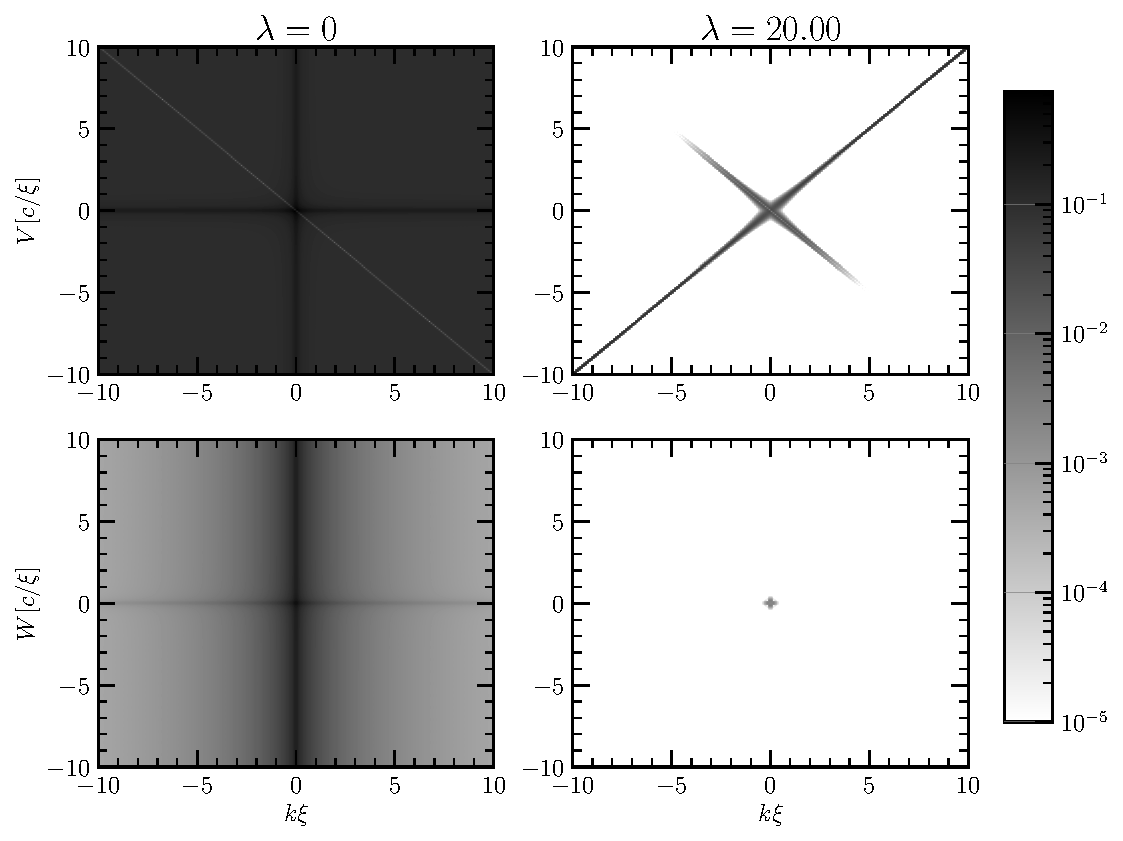
\includegraphics{figures/plots/PDF/FlowIllustration.pdf}
    \caption{Visualization of how the flow progresses for $\eta=10$ by shading larger absolute values for $V_{k,k^\prime},W_{k,k^\prime}$ darker. We see that good suppression occurs for all $W_{k,k^\prime}$, with slower convergence for smaller $|k|,|k^\prime|$.  Meanwhile, the matrix elements near the diagonal $V_{k,k}$ decay significantly slower than most off-diagonal elements. Also, matrix elements $V_{k,-k}$ converge, but to a value different from zero.}
    \label{FlowIllustration}
\end{figure}
As seen in figure \ref{FlowIllustration}

%%% CONCLUSION
\chapter{Conclusion}
\thispagestyle{empty}




%%% APPENDIX
\begin{appendix}

\chapter{Detailed Calculations}
\thispagestyle{empty}

\section{Deriving the flow equations in the case of no n-dependence}
First the canonical generator $\hat\eta$ has to be evaluated:
\begin{align}
\hat\eta&\defeq\hat\eta(\lambda)\defeq\left[\ham_0,\ham_{\mathrm{int}}\right] = \left[\Sum_k \omega_k \CR_k\AN_k,\Sum_{q\neq q^\prime}V_{q,q^\prime}\CR_q\AN_{q^\prime}+\Sum_{p,p^\prime}\left(W_{p,p^\prime}\CR_p\CR_{p^\prime}+W_{p,p^\prime}^*\AN_p\AN_{p^\prime}\right)\right]  \\ \quad& 
= \Sum_k\Sum_{q,q^\prime}\omega_kV_{q,q^\prime}\left[\CR_k\AN_k,\CR_q\AN_{q^\prime}\right]+\Sum_k\Sum_{p,p^\prime}\left(\omega_k W_{p,p^\prime}\left[\CR_k\AN_k,\CR_p\CR_{p^\prime}\right]+\omega_k W_{p,p^\prime}^*\left[\CR_k\AN_k,\AN_p\AN_{p^\prime}\right]\right) \nonumber \\ \quad& 
=\Sum_k\Sum_{q,q^\prime}\omega_kV_{q,q^\prime}\left(\CR_k\AN_{q^\prime}\delta_{k,q}-\CR_q\AN_k\delta_{k,q^\prime}\right) \nonumber \\ \quad& +\Sum_k\Sum_{p,p^\prime}\left(\omega_k W_{p,p^\prime}\left(\CR_k\CR_p\delta_{k,p^\prime}+\CR_k\CR_{p^\prime}\delta_{k,p}\right)-\omega_k W_{p,p^\prime}^*\left(\AN_p\AN_k\delta_{k,p^\prime}+\AN_{p^\prime}\AN_k\delta_{k,p}\right)\right) \nonumber \\ \quad& = \Sum_{q\neq q^\prime}V_{q,q^\prime}(\omega_q-\omega_{q^\prime})\CR_q\AN_{q^\prime}+\Sum_{p,p^\prime}\left(W_{p,p^\prime}(\omega_p+\omega_{p^\prime})\CR_p\CR_{p^\prime}-W_{p,p^\prime}^*(\omega_p+\omega_{p^\prime})\AN_p\AN_{p^\prime}\right) \label{eta_wo_n_final}
\end{align}
Since $\hat\eta$ has the same form as $\ham_{\mathrm{int}}$, $\left[\hat\eta,\ham_0\right]$ follows by inspection of \ref{eta_wo_n_final}:
\begin{align}
\left[\hat\eta,\ham_0\right]&=-\Sum_{q\neq q^\prime}V_{q,q^\prime}(\omega_q-\omega_{q^\prime})^2\CR_q\AN_{q^\prime}\nonumber \\ \quad& -\Sum_{p,p^\prime}\left(W_{p,p^\prime}(\omega_p+\omega_{p^\prime})^2\CR_p\CR_{p^\prime}+W_{p,p^\prime}^*(\omega_p+\omega_{p^\prime})^2\AN_p\AN_{p^\prime}\right) 
\end{align}
The commutator of the generator and $\ham_{\mathrm{int}}$ needs more work:
\begin{align}
\left[\hat\eta,\ham_{\mathrm{int}}\right]&=\Bigg[\Sum_{q\neq q^\prime}V_{q,q^\prime}(\omega_q-\omega_{q^\prime})\CR_q\AN_{q^\prime} +\Sum_{p,p^\prime}\big(W_{p,p^\prime}(\omega_p+\omega_{p^\prime})\CR_p\CR_{p^\prime}\\ \quad&-W_{p,p^\prime}^*(\omega_p+\omega_{p^\prime})\AN_p\AN_{p^\prime}\big),
\Sum_{\tilde q\neq \tilde q^\prime}V_{\tilde q,\tilde q^\prime}\CR_{\tilde q}\AN_{\tilde q^\prime}+\Sum_{\tilde p,\tilde p^\prime}\left(W_{\tilde p,\tilde p^\prime}\CR_{\tilde p}\CR_{\tilde p^\prime}+W_{\tilde p,\tilde p^\prime}^*\AN_{\tilde p}\AN_{\tilde p^\prime}\right)\Bigg]\nonumber\\ \quad& 
=\left[\Sum_{q\neq q^\prime}V_{q,q^\prime}(\omega_q-\omega_{q^\prime})\CR_q\AN_{q^\prime} , \Sum_{\tilde q\neq \tilde q^\prime}V_{\tilde q,\tilde q^\prime}\CR_{\tilde q}\AN_{\tilde q^\prime} \right] \label{wo_n_I} \\ \quad&
+\left[\Sum_{q\neq q^\prime}V_{q,q^\prime}(\omega_q-\omega_{q^\prime})\CR_q\AN_{q^\prime},\Sum_{\tilde p,\tilde p^\prime}\left(W_{\tilde p,\tilde p^\prime}\CR_{\tilde p}\CR_{\tilde p^\prime}+W_{\tilde p,\tilde p^\prime}^*\AN_{\tilde p}\AN_{\tilde p^\prime}\right)\right] \label{wo_n_II} \\ \quad&
+\left[\Sum_{p,p^\prime}\left(W_{p,p^\prime}(\omega_p+\omega_{p^\prime})\CR_p\CR_{p^\prime}-W_{p,p^\prime}^*(\omega_p+\omega_{p^\prime})\AN_p\AN_{p^\prime}\right),\Sum_{\tilde q\neq \tilde q^\prime}V_{\tilde q,\tilde q^\prime}\CR_{\tilde q}\AN_{\tilde q^\prime}\right] \label{wo_n_III}\\ \quad&
+\left[\Sum_{p,p^\prime}\left(W_{p,p^\prime}(\omega_p+\omega_{p^\prime})\CR_p\CR_{p^\prime}-W_{p,p^\prime}^*(\omega_p+\omega_{p^\prime})\AN_p\AN_{p^\prime}\right),\Sum_{\tilde p,\tilde p^\prime}\left(W_{\tilde p,\tilde p^\prime}\CR_{\tilde p}\CR_{\tilde p^\prime}+W_{\tilde p,\tilde p^\prime}^*\AN_{\tilde p}\AN_{\tilde p^\prime}\right)\right] \label{wo_n_IV}
\end{align}
In the following, \ref{wo_n_I}-\ref{wo_n_IV} will be evaluated separately. There will occur sums with $V_{q,q^\prime}$ where $q=q^\prime$. In this case, we define $V_{k,k}\defeq 0\ \forall k$. This saves the rather tedious declaration of the constraints of several sum indices.
\begin{itemize}
\item [\textbf{\ref{wo_n_I}:}] \begin{align}&\left[\Sum_{q\neq q^\prime}V_{q,q^\prime}(\omega_q-\omega_{q^\prime})\CR_q\AN_{q^\prime} , \Sum_{\tilde q\neq \tilde q^\prime}V_{\tilde q,\tilde q^\prime}\CR_{\tilde q}\AN_{\tilde q^\prime} \right] \nonumber \\ \quad& = \Sum_{q\neq q^\prime}\Sum_{\tilde q\neq \tilde q^\prime}V_{\tilde q,\tilde q^\prime}V_{q,q^\prime}(\omega_q-\omega_{q^\prime})\left[\CR_q\AN_{q^\prime} , \CR_{\tilde q}\AN_{\tilde q^\prime} \right] \nonumber \\ \quad& =  \Sum_{q\neq q^\prime}\Sum_{\tilde q\neq \tilde q^\prime}V_{\tilde q,\tilde q^\prime}V_{q,q^\prime}(\omega_q-\omega_{q^\prime})\left(\CR_q\AN_{\tilde q^\prime}\delta_{q^\prime,\tilde q}-\CR_{\tilde q}\AN_{q^\prime}\delta_{q,\tilde q^\prime}\right) \nonumber \\ \quad& 
= \Sum_{q\neq q^\prime}\Sum_{\tilde q^\prime}V_{q^\prime,\tilde q^\prime}V_{q,q^\prime}(\omega_q-\omega_{q^\prime})\CR_q\AN_{\tilde q^\prime} - \Sum_{q\neq q^\prime}\Sum_{\tilde q}V_{\tilde q,q}V_{q,q^\prime}(\omega_q-\omega_{q^\prime})\CR_{\tilde q}\AN_{q^\prime} \nonumber \\ \quad& 
= \Sum_{q, q^\prime}\Sum_{\tilde q^\prime}V_{q^\prime,\tilde q^\prime}V_{q,q^\prime}(\omega_q-\omega_{q^\prime})\CR_q\AN_{\tilde q^\prime} - \Sum_{q,q^\prime}\Sum_{\tilde q}V_{\tilde q,q}V_{q,q^\prime}(\omega_q-\omega_{q^\prime})\CR_{\tilde q}\AN_{q^\prime} \nonumber \\ \quad& 
=  \Sum_{q, q^\prime}\Sum_{\tilde q}V_{\tilde q,q^\prime}V_{q,\tilde q}(\omega_q-\omega_{\tilde q})\CR_q\AN_{q^\prime} - \Sum_{q,q^\prime}\Sum_{\tilde q}V_{q,\tilde q}V_{\tilde q,q^\prime}(\omega_{\tilde q}-\omega_{q^\prime})\CR_{q}\AN_{q^\prime} \nonumber \\ \quad& 
=\Sum_{q\neq q^\prime}\Sum_{\tilde q}V_{\tilde q,q^\prime}V_{q,\tilde q}(\omega_q-\omega_{\tilde q})\CR_q\AN_{q^\prime} - \Sum_{q\neq q^\prime}\Sum_{\tilde q}V_{q,\tilde q}V_{\tilde q,q^\prime}(\omega_{\tilde q}-\omega_{q^\prime})\CR_{q}\AN_{q^\prime} \nonumber \\ \quad& + \Sum_{k}\Sum_{\tilde q}V_{\tilde q,k}V_{k,\tilde q}(\omega_k-\omega_{\tilde q})\CR_k\AN_{k} - \Sum_{k}\Sum_{\tilde q}V_{k,\tilde q}V_{\tilde q,k}(\omega_{\tilde q}-\omega_{k})\CR_{k}\AN_{k} \nonumber \\ \quad& 
=\Sum_{q\neq q^\prime}\Sum_{\tilde q}V_{\tilde q,q^\prime}V_{q,\tilde q}(\omega_q-\omega_{\tilde q})\CR_q\AN_{q^\prime} - \Sum_{q\neq q^\prime}\Sum_{\tilde q}V_{q,\tilde q}V_{\tilde q,q^\prime}(\omega_{\tilde q}-\omega_{q^\prime})\CR_{q}\AN_{q^\prime} \nonumber \\ \quad& + \Sum_{k}\Sum_{\tilde q}2V_{\tilde q,k}V_{k,\tilde q}(\omega_k-\omega_{\tilde q})\CR_k\AN_{k}
\end{align}
\item [\textbf{\ref{wo_n_II}:}]
\begin{align}
&\left[\Sum_{q\neq q^\prime}V_{q,q^\prime}(\omega_q-\omega_{q^\prime})\CR_q\AN_{q^\prime},\Sum_{\tilde p,\tilde p^\prime}\left(W_{\tilde p,\tilde p^\prime}\CR_{\tilde p}\CR_{\tilde p^\prime}+W_{\tilde p,\tilde p^\prime}^*\AN_{\tilde p}\AN_{\tilde p^\prime}\right)\right] \nonumber \\ \quad&
= \Sum_{q\neq q^\prime}\Sum_{\tilde p,\tilde p^\prime}V_{q,q^\prime}(\omega_q-\omega_{q^\prime})\left(W_{\tilde p,\tilde p^\prime}\left[\CR_q\AN_{q^\prime},\CR_{\tilde p}\CR_{\tilde p^\prime}\right]+W_{\tilde p,\tilde p^\prime}^*\left[\CR_q\AN_{q^\prime},\AN_{\tilde p}\AN_{\tilde p^\prime}\right]\right)\nonumber \\ \quad& 
= \Sum_{q,q^\prime}\Sum_{\tilde p,\tilde p^\prime}V_{q,q^\prime}(\omega_q-\omega_{q^\prime})\left(W_{\tilde p,\tilde p^\prime}\left(\CR_q\CR_{\tilde p}\delta_{q^\prime,\tilde p^\prime}+ \CR_q\CR_{\tilde p^\prime}\delta_{q^\prime,\tilde p}\right)-W_{\tilde p,\tilde p^\prime}^*\AN_{\tilde p}\left(\AN_{\tilde p^\prime}\AN_{q^\prime}\delta_{q,\tilde p}+\AN_{\tilde p}\AN_{q^\prime}\delta_{\tilde p^\prime,q}\right)\right)\nonumber \\ \quad&
= \Sum_{ p, p^\prime}\Sum_{q}V_{q,p^\prime}(\omega_q-\omega_{p^\prime}) W_{ p, p^\prime}\CR_q\CR_{ p}
+\Sum_{ p, p^\prime}\Sum_{q}V_{q,p}(\omega_q-\omega_{p}) W_{ p, p^\prime} \CR_q\CR_{ p^\prime} \nonumber \\ \quad& 
-\Sum_{ p, p^\prime}\Sum_{q^\prime}V_{p,q^\prime}(\omega_p-\omega_{q^\prime}) W_{ p, p^\prime}^* \AN_{ p^\prime}\AN_{q^\prime}
-\Sum_{ p, p^\prime}\Sum_{q^\prime}V_{p^\prime,q^\prime}(\omega_{p^\prime}-\omega_{q^\prime}) W_{ p, p^\prime}^* \AN_{ p}\AN_{q^\prime} \nonumber \\ \quad& 
= \Sum_{ p, p^\prime}\Sum_{q}V_{{p^\prime},q}(\omega_{p^\prime}-\omega_{q}) W_{ p, q}\CR_{ p}\CR_{p^\prime}
+\Sum_{ p, p^\prime}\Sum_{q}V_{p,q}(\omega_p-\omega_{q}) W_{ q, p^\prime} \CR_p\CR_{ p^\prime} \nonumber \\ \quad& 
-\Sum_{ p, p^\prime}\Sum_{q}V_{q,p}(\omega_{q}-\omega_{p}) W_{ q, p^\prime}^* \AN_{p}\AN_{ p^\prime}
-\Sum_{ p, p^\prime}\Sum_{q}V_{q,p^\prime}(\omega_{q}-\omega_{p^\prime}) W_{ p, {q}}^* \AN_{ p}\AN_{p^\prime} \nonumber \\ \quad& 
= \Sum_{ p, p^\prime}\Sum_{q}V_{{p^\prime},q}(\omega_{p^\prime}-\omega_{q}) W_{ p, q}\CR_{ p}\CR_{p^\prime}
+\Sum_{ p, p^\prime}\Sum_{q}V_{p,q}(\omega_p-\omega_{q}) W_{ q, p^\prime} \CR_p\CR_{ p^\prime} \nonumber \\ \quad& 
-\Sum_{ p, p^\prime}\Sum_{q}V_{q,p}(\omega_{q}-\omega_{p}) W_{ q, p^\prime}^* \AN_{p}\AN_{ p^\prime}
-\Sum_{ p, p^\prime}\Sum_{q}V_{q,p^\prime}(\omega_{q}-\omega_{p^\prime}) W_{ p, {q}}^* \AN_{ p}\AN_{p^\prime} \nonumber \\ \quad& 
=\Sum_{ p, p^\prime}\Sum_{q}V_{{p},q}(\omega_{p}-\omega_{q}) (W_{ q, p^\prime}+W_{ p^\prime, q})\CR_{ p}\CR_{p^\prime}\nonumber \\ \quad& 
+\Sum_{ p, p^\prime}\Sum_{q}V_{q,p}(\omega_{p}-\omega_{q}) (W_{ q, p^\prime}^*+W_{ p^\prime, {q}}^*) \AN_{p}\AN_{ p^\prime}
%= \Sum_{ p, p^\prime}\Sum_{q}V_{p,q}(\omega_{p^\prime}+\omega_p-2\omega_{q}) W_{ q, p^\prime} \CR_p\CR_{ p^\prime} \nonumber \\ \quad& 
%+\Sum_{ p, p^\prime}\Sum_{q}V_{q,p^\prime}(\omega_{p^\prime}+\omega_p-2\omega_{q}) W_{ p, {q}}^* \AN_{ p}\AN_{p^\prime} \nonumber \\ \quad& 
%= \Sum_{ p, p^\prime}\Sum_{q}V_{p,q}(\omega_{p^\prime}+\omega_p-2\omega_{q}) W_{ q, p^\prime} \CR_p\CR_{ p^\prime} \nonumber \\ \quad& 
%+\Sum_{ p, p^\prime}\Sum_{q}V_{q,p}(\omega_{p^\prime}+\omega_p-2\omega_{q}) W_{ p^\prime, {q}}^* \AN_{ p}\AN_{p^\prime}
\end{align}
\item [\textbf{\ref{wo_n_III}:}]
\begin{align}
&\left[\Sum_{p,p^\prime}\left(W_{p,p^\prime}(\omega_p+\omega_{p^\prime})\CR_p\CR_{p^\prime}-W_{p,p^\prime}^*(\omega_p+\omega_{p^\prime})\AN_p\AN_{p^\prime}\right),\Sum_{\tilde q\neq \tilde q^\prime}V_{\tilde q,\tilde q^\prime}\CR_{\tilde q}\AN_{\tilde q^\prime}\right]\nonumber \\ \quad& 
=\Sum_{p,p^\prime}\Sum_{\tilde q\neq \tilde q^\prime}V_{\tilde q,\tilde q^\prime}(\omega_p+\omega_{p^\prime})\left(W_{p,p^\prime}\left[\CR_p\CR_{p^\prime},\CR_{\tilde q}\AN_{\tilde q^\prime}\right]-W_{p,p^\prime}^*\left[\AN_p\AN_{p^\prime},\CR_{\tilde q}\AN_{\tilde q^\prime}\right]\right)\nonumber \\ \quad& 
=-\Sum_{p,p^\prime}\Sum_{ q\neq  q^\prime}V_{ q, q^\prime}(\omega_p+\omega_{p^\prime})W_{p,p^\prime}\left(\CR_q\CR_p\delta_{q^\prime,p^\prime}+\CR_q\CR_{p^\prime}\delta_{q^\prime,p}\right)\nonumber \\ \quad& 
-\Sum_{p,p^\prime}\Sum_{ q\neq  q^\prime}V_{ q, q^\prime}(\omega_p+\omega_{p^\prime})W_{p,p^\prime}^*\left(\AN_p\AN_{q^\prime}\delta_{q,p^\prime}+\AN_{p^\prime}\AN_{q^\prime}\delta_{q,p}\right)\nonumber \\ \quad& 
=-\Sum_{p,p^\prime}\Sum_{q}V_{ q, p^\prime}(\omega_p+\omega_{p^\prime})W_{p,p^\prime}\CR_q\CR_p
-\Sum_{p,p^\prime}\Sum_{ q}V_{ q, p}(\omega_p+\omega_{p^\prime})W_{p,p^\prime}\CR_q\CR_{p^\prime} \nonumber \\ \quad& 
-\Sum_{p,p^\prime}\Sum_{ q^\prime}V_{ p^\prime, q^\prime}(\omega_p+\omega_{p^\prime})W_{p,p^\prime}^*\AN_p\AN_{q^\prime}
-\Sum_{p,p^\prime}\Sum_{ q^\prime}V_{ p, q^\prime}(\omega_p+\omega_{p^\prime})W_{p,p^\prime}^*\AN_{p^\prime}\AN_{q^\prime}\nonumber \\ \quad& 
=-\Sum_{p,p^\prime}\Sum_{q}V_{ {p^\prime},q}(\omega_p+\omega_{q})W_{p,q}\CR_p\CR_{p^\prime}
-\Sum_{p,p^\prime}\Sum_{ q}V_{ p, q}(\omega_q+\omega_{p^\prime})W_{q,p^\prime}\CR_p\CR_{p^\prime} \nonumber \\ \quad& 
-\Sum_{p,p^\prime}\Sum_{ q^\prime}V_{ q^\prime, p^\prime}(\omega_p+\omega_{q^\prime})W_{p,q^\prime}^*\AN_p\AN_{p^\prime}
-\Sum_{p,p^\prime}\Sum_{ q^\prime}V_{ q^\prime, p}(\omega_{q^\prime}+\omega_{p^\prime})W_{q^\prime,p^\prime}^*\AN_{p}\AN_{p^\prime}\nonumber \\ \quad& 
=-\Sum_{p,p^\prime}\Sum_{ q}V_{ p, q}(\omega_q+\omega_{p^\prime})(W_{p^\prime,q}+W_{q,p^\prime})\CR_p\CR_{p^\prime} \nonumber \\ \quad& 
-\Sum_{p,p^\prime}\Sum_{ q}V_{ q, p}(\omega_{q}+\omega_{p^\prime})(W_{p^\prime,q}^*+W_{q,p^\prime}^*)\AN_{p}\AN_{p^\prime}
\end{align}
\item [\textbf{\ref{wo_n_IV}:}]
\begin{align}
&\left[\Sum_{p,p^\prime}\left(W_{p,p^\prime}(\omega_p+\omega_{p^\prime})\CR_p\CR_{p^\prime}-W_{p,p^\prime}^*(\omega_p+\omega_{p^\prime})\AN_p\AN_{p^\prime}\right),\Sum_{\tilde p,\tilde p^\prime}\left(W_{\tilde p,\tilde p^\prime}\CR_{\tilde p}\CR_{\tilde p^\prime}+W_{\tilde p,\tilde p^\prime}^*\AN_{\tilde p}\AN_{\tilde p^\prime}\right)\right] \nonumber \\ \quad& 
=\Sum_{p,p^\prime}\Sum_{\tilde p,\tilde p^\prime}W_{p,p^\prime}(\omega_p+\omega_{p^\prime})W_{\tilde p,\tilde p^\prime}^*\left[\CR_p\CR_{p^\prime},\AN_{\tilde p}\AN_{\tilde p^\prime}\right]
-\Sum_{p,p^\prime}\Sum_{\tilde p,\tilde p^\prime} W_{p,p^\prime}^*W_{\tilde p,\tilde p^\prime}(\omega_p+\omega_{p^\prime})\left[\AN_p\AN_{p^\prime},\CR_{\tilde p}\CR_{\tilde p^\prime}\right] \nonumber \\ \quad& 
=-\Sum_{p,p^\prime}\Sum_{\tilde p,\tilde p^\prime}W_{p,p^\prime}(\omega_p+\omega_{p^\prime}+\omega_{\tilde p}+\omega_{\tilde p^\prime})W_{\tilde p,\tilde p^\prime}^*\left[\AN_{\tilde p}\AN_{\tilde p^\prime},\CR_p\CR_{p^\prime}\right] \nonumber \\ \quad& 
=-\Sum_{p,p^\prime}\Sum_{\tilde p,\tilde p^\prime}W_{p,p^\prime}(\omega_p+\omega_{p^\prime}+\omega_{\tilde p}+\omega_{\tilde p^\prime})W_{\tilde p,\tilde p^\prime}^*\AN_{\tilde p}\CR_p\delta_{\tilde p^\prime,p^\prime}\nonumber \\ \quad& 
-\Sum_{p,p^\prime}\Sum_{\tilde p,\tilde p^\prime}W_{p,p^\prime}(\omega_p+\omega_{p^\prime}+\omega_{\tilde p}+\omega_{\tilde p^\prime})W_{\tilde p,\tilde p^\prime}^*\AN_{\tilde p}\CR_{p^\prime}\delta_{\tilde p^\prime,p}\nonumber \\ \quad& 
-\Sum_{p,p^\prime}\Sum_{\tilde p,\tilde p^\prime}W_{p,p^\prime}(\omega_p+\omega_{p^\prime}+\omega_{\tilde p}+\omega_{\tilde p^\prime})W_{\tilde p,\tilde p^\prime}^*\CR_p\AN_{\tilde p^\prime}\delta_{\tilde p,p^\prime}\nonumber \\ \quad& 
-\Sum_{p,p^\prime}\Sum_{\tilde p,\tilde p^\prime}W_{p,p^\prime}(\omega_p+\omega_{p^\prime}+\omega_{\tilde p}+\omega_{\tilde p^\prime})W_{\tilde p,\tilde p^\prime}^*\CR_{p^\prime}\AN_{\tilde p^\prime}\delta_{\tilde p,p}\nonumber \\ \quad& 
=-\Sum_{p,p^\prime}\Sum_{\tilde p}W_{p,p^\prime}(\omega_p+2\omega_{p^\prime}+\omega_{\tilde p})W_{\tilde p,p^\prime}^*\AN_{\tilde p}\CR_p
-\Sum_{p,p^\prime}\Sum_{\tilde p}W_{p,p^\prime}(2\omega_p+\omega_{p^\prime}+\omega_{\tilde p})W_{\tilde p,p}^*\AN_{\tilde p}\CR_{p^\prime}\nonumber \\ \quad& 
-\Sum_{p,p^\prime}\Sum_{\tilde p^\prime}W_{p,p^\prime}(\omega_p+2\omega_{p^\prime}+\omega_{\tilde p^\prime})W_{p^\prime,\tilde p^\prime}^*\CR_p\AN_{\tilde p^\prime}
-\Sum_{p,p^\prime}\Sum_{\tilde p^\prime}W_{p,p^\prime}(2\omega_p+\omega_{p^\prime}+\omega_{\tilde p^\prime})W_{p,\tilde p^\prime}^*\CR_{p^\prime}\AN_{\tilde p^\prime}\nonumber \\ \quad& 
=-\Sum_{p,p^\prime}\Sum_{\tilde p}W_{p,\tilde p}(\omega_p+2\omega_{\tilde p}+\omega_{p^\prime})W_{p^\prime,\tilde p}^*\AN_{p^\prime}\CR_p
-\Sum_{p,p^\prime}\Sum_{\tilde p}W_{\tilde p,p}(2\omega_{\tilde p}+\omega_{p}+\omega_{p^\prime})W_{p^\prime,\tilde p}^*\AN_{p^\prime}\CR_{p}\nonumber \\ \quad& 
-\Sum_{p,p^\prime}\Sum_{\tilde p^\prime}W_{p,\tilde p^\prime}(\omega_p+2\omega_{\tilde p^\prime}+\omega_{ p^\prime})W_{\tilde p^\prime, p^\prime}^*\CR_p\AN_{ p^\prime}
-\Sum_{p,p^\prime}\Sum_{\tilde p^\prime}W_{\tilde p^\prime,p}(2\omega_{\tilde p^\prime}+\omega_p+\omega_{p^\prime})W_{\tilde p^\prime,{p^\prime}}^*\CR_p\AN_{p^\prime}\nonumber \\ \quad& 
=-\Sum_{p,p^\prime}\Sum_{\tilde p}(W_{p,\tilde p}+W_{\tilde p,p})(\omega_p+2\omega_{\tilde p}+\omega_{p^\prime})W_{p^\prime,\tilde p}^*\AN_{p^\prime}\CR_p\nonumber \\ \quad& 
-\Sum_{p,p^\prime}\Sum_{\tilde p^\prime}(W_{p,\tilde p^\prime}+W_{\tilde p^\prime,p})(\omega_p+2\omega_{\tilde p^\prime}+\omega_{ p^\prime})W_{\tilde p^\prime, p^\prime}^*\CR_p\AN_{ p^\prime}\nonumber \\ \quad& 
=-\Sum_{p,p^\prime}\Sum_{\tilde p}(W_{p,\tilde p}+W_{\tilde p,p})(\omega_p+2\omega_{\tilde p}+\omega_{p^\prime})W_{p^\prime,\tilde p}^*(\delta_{p,p^\prime}+\CR_p\nonumber\AN_{p^\prime}) \\ \quad& 
-\Sum_{p,p^\prime}\Sum_{\tilde p}(W_{p,\tilde p}+W_{\tilde p,p})(\omega_p+2\omega_{\tilde p}+\omega_{ p^\prime})W_{\tilde p, p^\prime}^*\CR_p\AN_{ p^\prime}\nonumber \\ \quad& 
= -\Sum_{p,p^\prime}\Sum_{\tilde p}(W_{p,\tilde p}+W_{\tilde p,p})(\omega_p+2\omega_{\tilde p}+\omega_{ p^\prime})(W_{\tilde p, p^\prime}^*+W_{p^\prime,\tilde p}^*)\CR_p\AN_{ p^\prime}\nonumber \\ \quad& 
-2\Sum_{k}\Sum_{\tilde p}(W_{k,\tilde p}+W_{\tilde p,k})(\omega_k+\omega_{\tilde p})W_{k,\tilde p}^*\nonumber \\ \quad& 
= -\Sum_{q\neq q^\prime}\Sum_{\tilde p}(W_{q,\tilde p}+W_{\tilde p,q})(\omega_q+2\omega_{\tilde p}+\omega_{ q^\prime})(W_{\tilde p, q^\prime}^*+W_{q^\prime,\tilde p}^*)\CR_q\AN_{ q^\prime}\nonumber \\ \quad& 
-2\Sum_{k}\Sum_{\tilde p}(W_{k,\tilde p}+W_{\tilde p,k})(\omega_k+\omega_{\tilde p})(W_{\tilde p, k}^*+W_{k,\tilde p}^*)\CR_k\AN_{ k}\nonumber \\ \quad& 
-2\Sum_{k}\Sum_{\tilde p}(W_{k,\tilde p}+W_{\tilde p,k})(\omega_k+\omega_{\tilde p})W_{k,\tilde p}^*
\end{align}
\end{itemize}
We conclude that $\ham(\lambda)$ is of the form 
\begin{align}
\ham(\lambda)=\Sum_k \omega_k(\lambda) \CR_k\AN_k+\Sum_{q\neq q^\prime}V_{q,q^\prime}(\lambda)\CR_q\AN_{q^\prime}+\Sum_{p,p^\prime}\left(W_{p,p^\prime}(\lambda)\CR_p\CR_{p^\prime}+W_{p,p^\prime}^*(\lambda)\AN_p\AN_{p^\prime}\right)+\epsilon(\lambda)
\end{align}
where $\epsilon(\lambda)$ is a constant shift in the energy scale.\\
Using the expressions for the commutators of the generator and $\ham_0$ respectively $\ham_{\mathrm{int}}$ derived above, the flow $\partial_\lambda\ham(\lambda)=[\hat\eta(\lambda),\ham(\lambda)]$ yields the following flow equations $\forall k, p,p^\prime, q, q^\prime$ where $q\neq q^\prime$:
\begin{flushleft}
\begin{subequations}
\begin{align}
\partial_\lambda\omega_k&= \Sum_{\tilde q}2V_{\tilde q,k}V_{k,\tilde q}(\omega_k-\omega_{\tilde q})-2\Sum_{\tilde p}(W_{k,\tilde p}+W_{\tilde p,k})(\omega_k+\omega_{\tilde p})(W_{\tilde p, k}^*+W_{k,\tilde p}^*)\label{feq_won_I}\\ 
\partial_\lambda V_{q,q^\prime}&=-V_{q,q^\prime}(\omega_q-\omega_{q^\prime})^2-\Sum_{\tilde p}(W_{q,\tilde p}+W_{\tilde p,q})(\omega_q+\omega_{ q^\prime}+2\omega_{\tilde p})(W_{\tilde p, q^\prime}^*+W_{q^\prime,\tilde p}^*) \nonumber\\ \quad&
+ \Sum_{\tilde q}V_{\tilde q,q^\prime}V_{q,\tilde q}(\omega_q+\omega_{q^\prime}-2\omega_{\tilde q}) %- \Sum_{\tilde q}V_{q,\tilde q}V_{\tilde q,q^\prime}(\omega_{\tilde q}-\omega_{q^\prime})
\label{feq_won_II} \\ 
\partial_\lambda W_{p,p^\prime}&=-W_{p,p^\prime}(\omega_p+\omega_{p^\prime})^2-\Sum_{ q}V_{ p, q}(\omega_q+\omega_{p^\prime})(W_{p^\prime,q}+W_{q,p^\prime}) \nonumber\\ \quad&
+ \Sum_{q}V_{{p},q}(\omega_{p}-\omega_{q}) (W_{ q, p^\prime}+W_{ p^\prime, q})\label{feq_won_III}\\ 
\partial_\lambda W_{p,p^\prime}^*&=-W_{p,p^\prime}^*(\omega_p+\omega_{p^\prime})^2-\Sum_{ q}V_{ q, p}(\omega_{q}+\omega_{p^\prime})(W_{p^\prime,q}^*+W_{q,p^\prime}^*)\nonumber\\ \quad& 
+\Sum_{q}V_{q,p}(\omega_{p}-\omega_{q}) (W_{ q, p^\prime}^*+W_{ p^\prime, {q}}^*)\label{feq_won_III'}\\ 
\partial_\lambda \varepsilon&=-2\Sum_{p,p^\prime}(W_{p,p^\prime}+W_{p^\prime,p})(\omega_p+\omega_{p^\prime})W_{p,p^\prime}^*\label{feq_won_IV}
\end{align}
\end{subequations}
\end{flushleft}
Obviously, equations \ref{feq_won_III} and \ref{feq_won_III'} are not independent from each other, since they are related by complex conjugation. Seeing this is a good consistency check because complex conjugation was not explicitly used in the derivation of the these two equations.\\
Furthermore note that in first order the flow equations \ref{feq_won_I}-\ref{feq_won_IV} suggest that they are exact in the sense that if the flow is completely traversed, the flow Hamiltonian will be exactly diagonal.

\section{Deriving the flow equations with n-dependence}
\subsection{Useful preliminaries}
Consider some operator $\hat f$ which depends on a number operator $\hat n=\CR\AN$. The following relations will be used later:
\begin{subequations}
\label{fcom}
\begin{align}
\left[\CR,\hat f(\hat n) \right] &= \CR\left(\hat f(\hat n)-\hat f(\hat n+1)\right)\\ 
\left[\AN,\hat f(\hat n) \right] &= \AN\left(\hat f(\hat n)-\hat f(\hat n-1)\right)\\
\left[\hat f(\hat n),\CR \right] &= \left(\hat f(\hat n)-\hat f(\hat n-1)\right)\CR\\
\left[\hat f(\hat n),\AN \right] &= \left(\hat f(\hat n)-\hat f(\hat n+1)\right)\AN
\end{align}
\end{subequations}
These can be proved by induction for $\hat f(\hat n)=\hat n^k, k\in\N$ and from there simply extended to well-behaved $\hat f$ via power series. Equations \ref{fcom} are still valid for functions depending on $\left\{\hat n_k\right\}_k$, because all $\hat n_k$ pairwise commute.\\
We will write $\hat f\left(\hat n_1,\hat n_2,\hdots\right)\eqdef \hat f$ and $\hat f\left(\hat n_1,\hat n_2,\hdots,\hat n_k\pm 1,\hat n_{k+1},\hdots\right)\eqdef \hat f(\hat n_k\pm1)$. In this notation it is understood that $\hat f(\hat n_k\pm1,\hat n_{k}\pm1)\eqdef\hat f(\hat n_k\pm2)$.\\
Using this notation, it is evident that a simple induction for $n_1,n_2\in\N_0$ yields the following relation:
\begin{align}
&\left[\hat f(\hat n),\CR_{k_1}\CR_{k_2}\cdots\CR_{k_{n_1}}\AN_{k_1}\AN_{k_2}\cdots\AN_{k_{n_2}} \right] \nonumber \\ \quad& 
= \left(\hat f-\hat f\left(\hat n_{k_1}-1,\hat n_{k_2}-1,\hdots,\hat n_{k_{n_1}},\hat n_{k_1}+1,\hat n_{k_2}+1\hdots\hat n_{k_{n_2}}+1\right)\right)\CR_{k_1}\CR_{k_2}\cdots\CR_{k_{n_1}}\AN_{k_1}\AN_{k_2}\cdots\AN_{k_{n_2}}
\end{align}
Furthermore, applying the recurrence relation introduced to define the normal ordering procedure can be used to successively normal order operators. Let $\hat O\defeq \CR_{k_1}\CR_{k_2}\cdots\CR_{k_{n_1}}\AN_{k_1}\AN_{k_2}\cdots\AN_{k_{n_2}}$. Then normal ordering w.r.t. the vacuum yields:
\begin{subequations}
\begin{align}
\AN_q\NO\hat O\NO &=\NO\hat O\AN_q\NO + \sum\limits_{k}\NO \frac{\partial \hat O}{\partial\CR_k}\NO \nonumber \\
 &= \NO\hat O\AN_q\NO + \sum\limits_{i=1}^{n_1}\delta_{k_i,q}\NO \CR_{k_1}\CR_{k_2}\cdots\CR_{k_{i-1}}\CR_{k_{i+1}}\cdots\CR_{k_{n_1}}\AN_{k_1}\AN_{k_2}\cdots\AN_{k_{n_2}}\NO \\
\CR_q\NO\hat O\NO &= \NO \CR_q\hat O\NO
\end{align}
\end{subequations}
\subsection{The canonical generator}
The first step in the calculating the flow equations is again to calculate the canonical commutator $\hat\eta\defeq\left[\ham_0,\ham_{\mathrm{int}}\right]$:
\begin{subequations}
\begin{align}
\hat\eta &= \left[\Sum_k \hat\omega_k \NO\CR_k\AN_k\NO,\Sum_{q\neq q^\prime}\hat V_{q,q^\prime}\NO \CR_q\AN_{q^\prime}\NO+\Sum_{p,p^\prime}\left(\hat W_{p,p^\prime}\NO \CR_p\CR_{p^\prime}\NO+\hat W_{p,p^\prime}^\dagger\NO\AN_p\AN_{p^\prime}\NO\right)\right]  \nonumber\\ \quad& 
= \Sum_k \Sum_{q\neq q^\prime}\left[ \hat\omega_k \NO\CR_k\AN_k\NO,\hat V_{q,q^\prime}\NO \CR_q\AN_{q^\prime}\NO\right] \label{eta_with_n_I}\\ \quad& 
+ \Sum_k\Sum_{p,p^\prime}\left[\hat\omega_k \NO\CR_k\AN_k\NO,\hat W_{p,p^\prime}\NO \CR_p\CR_{p^\prime}\NO\right] \label{eta_with_n_II} \\ \quad& 
+ \Sum_k\Sum_{p,p^\prime}\left[ \hat\omega_k \NO\CR_k\AN_k\NO,\hat W_{p,p^\prime}^\dagger\NO\AN_p\AN_{p^\prime} \NO \right] \label{eta_with_n_III}
\end{align}
\end{subequations}
In the following, the terms \ref{eta_with_n_I}-\ref{eta_with_n_III} will be evaluated separately:

\begin{itemize}
\item[\textbf{\ref{eta_with_n_I}}] 
\begin{align}
& \left[ \hat\omega_k \NO\CR_k\AN_k\NO,\hat V_{q,q^\prime}\NO \CR_q\AN_{q^\prime}\NO\right]\nonumber\\
&= \hat\omega_k \hat V_{q,q^\prime} \left[ \NO\CR_k\AN_k\NO,\NO \CR_q\AN_{q^\prime}\NO\right] + \hat\omega_k   \underbrace{\left[ \NO\CR_k\AN_k\NO,\hat V_{q,q^\prime}\right]}_{=0} \NO \CR_q\AN_{q^\prime}\NO \nonumber \\ 
&+ \hat V_{q,q^\prime} \left[ \hat\omega_k,\NO \CR_q\AN_{q^\prime}\NO\right]  \NO\CR_k\AN_k\NO + \underbrace{\left[ \hat\omega_k ,\hat V_{q,q^\prime}\right]}_{=0}\NO \CR_q\AN_{q^\prime}\NO \NO\CR_k\AN_k\NO \nonumber \\
&= \hat\omega_k \hat V_{q,q^\prime} \left(\NO\CR_k\AN_{q^\prime}\NO\delta_{k,q}-\NO\CR_q\AN_k\NO\delta_{k,q^\prime}\right) + \hat V_{q,q^\prime} \left(\hat\omega_k - \hat\omega_k(\hat n_q-1,\hat n_{q^\prime}+1)\right) \NO \CR_q\AN_{q^\prime}\NO \NO\CR_k\AN_k\NO\nonumber\\
&= \hat\omega_k \hat V_{q,q^\prime} \left(\NO\CR_k\AN_{q^\prime}\NO\delta_{k,q}-\NO\CR_q\AN_k\NO\delta_{k,q^\prime}\right) \nonumber \\
& + \hat V_{q,q^\prime} \left(\hat\omega_k - \hat\omega_k(\hat n_q-1,\hat n_{q^\prime}+1)\right) \left(\NO \CR_q\CR_k\AN_{q^\prime}\AN_k\NO+\delta_{q^\prime,k}\NO\CR_{q}\AN_k\NO\right)
\end{align}
\item[\textbf{\ref{eta_with_n_II}}] 
\begin{align}
&\left[\hat\omega_k \NO\CR_k\AN_k\NO,\hat W_{p,p^\prime}\NO \CR_p\CR_{p^\prime}\NO\right] \nonumber \\
&=\hat W_{p,p^\prime} \left[\hat\omega_k ,\NO \CR_p\CR_{p^\prime}\NO\right] \NO\CR_k\AN_k\NO + \hat W_{p,p^\prime}\hat\omega_k \left[ \NO\CR_k\AN_k\NO,\NO \CR_p\CR_{p^\prime}\NO\right] \nonumber\\
&= \hat W_{p,p^\prime} \left(\omega_k-\hat\omega(\hat n_{p^\prime}-1,\hat n_p -1)\right)\NO \CR_p\CR_{p^\prime}\NO\NO\CR_k\AN_k\NO + \hat W_{p,p^\prime}\hat\omega_k \left(\NO\CR_k\CR_p\NO\delta_{k,p^\prime}+\NO\CR_k\CR_{p^\prime}\NO\delta_{k,p}\right)\nonumber\\
&= \hat W_{p,p^\prime} \left(\omega_k-\hat\omega(\hat n_{p^\prime}-1,\hat n_p -1)\right)\NO \CR_p\CR_{p^\prime}\CR_k\AN_k\NO + \hat W_{p,p^\prime}\hat\omega_k \left(\NO\CR_k\CR_p\NO\delta_{k,p^\prime}+\NO\CR_k\CR_{p^\prime}\NO\delta_{k,p}\right)
\end{align}
\item[\textbf{\ref{eta_with_n_III}}] 
\begin{align}
&\left[ \hat\omega_k \NO\CR_k\AN_k\NO,\hat W_{p,p^\prime}^\dagger\NO\AN_p\AN_{p^\prime} \NO \right]\nonumber \\
&=\hat W_{p,p^\prime}^\dagger \left[ \hat\omega_k ,\NO\AN_p\AN_{p^\prime} \NO \right]\NO\CR_k\AN_k\NO+\hat W_{p,p^\prime}^\dagger \hat\omega_k\left[  \NO\CR_k\AN_k\NO,\NO\AN_p\AN_{p^\prime} \NO \right] \nonumber \\
&=\hat W_{p,p^\prime}^\dagger \left(\hat\omega_k-\hat\omega_k(\hat n_{p^\prime}+1,\hat n_p +1)\right)\NO \AN_p\AN_{p^\prime}\NO\NO\CR_k\AN_k\NO-\hat W_{p,p^\prime}^\dagger \hat\omega_k\left(\NO\AN_p\AN_k\NO\delta_{k,p^\prime}+\NO\AN_{p^\prime}\AN_k\NO\delta_{k,p}\right) \nonumber \\
&=\hat W_{p,p^\prime}^\dagger \left(\hat\omega_k-\hat\omega_k(\hat n_{p^\prime}+1,\hat n_p +1)\right)\left(\NO \CR_k\AN_k\AN_p\AN_{p^\prime}\NO+\delta_{k,p}\NO\AN_{p^\prime}\AN_k\NO+\delta_{k,p^\prime}\NO\AN_p\AN_k\NO\right) \nonumber \\
&-\hat W_{p,p^\prime}^\dagger \hat\omega_k\left(\NO\AN_p\AN_k\NO\delta_{k,p^\prime}+\NO\AN_{p^\prime}\AN_k\NO\delta_{k,p}\right)
\end{align}
\end{itemize}
This gives the canonical generator as:
\begin{align}
\hat\eta &= \Sum_k \Sum_{q\neq q^\prime}\Bigg(\hat\omega_k \hat V_{q,q^\prime} \left(\NO\CR_k\AN_{q^\prime}\NO\delta_{k,q}-\NO\CR_q\AN_k\NO\delta_{k,q^\prime}\right) \nonumber \\
& + \hat V_{q,q^\prime} \left(\hat\omega_k - \hat\omega_k(\hat n_q-1,\hat n_{q^\prime}+1)\right) \left(\NO \CR_q\CR_k\AN_{q^\prime}\AN_k\NO+\delta_{q^\prime,k}\NO\CR_{q}\AN_k\NO\right)\Bigg)\nonumber\\ \quad& 
+ \Sum_k\Sum_{p,p^\prime}\Bigg(\hat W_{p,p^\prime} \left(\hat\omega_k-\hat\omega_k(\hat n_{p^\prime}-1,\hat n_p -1)\right)\NO \CR_p\CR_{p^\prime}\CR_k\AN_k\NO + \hat W_{p,p^\prime}\hat\omega_k \left(\NO\CR_k\CR_p\NO\delta_{k,p^\prime}+\NO\CR_k\CR_{p^\prime}\NO\delta_{k,p}\right)\Bigg)\nonumber\\ \quad& 
+ \Sum_k\Sum_{p,p^\prime}\Bigg(\hat W_{p,p^\prime}^\dagger \left(\omega_k-\hat\omega_k(\hat n_{p^\prime}+1,\hat n_p +1)\right)\left(\NO \CR_k\AN_k\AN_p\AN_{p^\prime}\NO+\delta_{k,p}\NO\AN_{p^\prime}\AN_k\NO+\delta_{k,p^\prime}\NO\AN_p\AN_k\NO\right) \nonumber \\
&-\hat W_{p,p^\prime}^\dagger \hat\omega_k\left(\NO\AN_p\AN_k\NO\delta_{k,p^\prime}+\NO\AN_{p^\prime}\AN_k\NO\delta_{k,p}\right)\Bigg) \nonumber \\ \quad&
= \Sum_{q\neq q^\prime}(\hat\omega_q-\hat\omega_{q^\prime}(\hat n_q-1,\hat n_{q^\prime}+1))\hat V_{q,q^\prime}\NO\CR_q\AN_{q^\prime}\NO \nonumber \\\quad&
+\Sum_{q\neq q^\prime}\Sum_k \hat V_{q,q^\prime} \left(\hat\omega_k - \hat\omega_k(\hat n_q-1,\hat n_{q^\prime}+1)\right)\NO \CR_q\CR_k\AN_{q^\prime}\AN_k\NO \nonumber \\\quad&
+ \Sum_k\Sum_{p,p^\prime}\hat W_{p,p^\prime} \left(\omega_k-\hat\omega_k(\hat n_{p^\prime}-1,\hat n_p -1)\right)\NO \CR_p\CR_{p^\prime}\CR_k\AN_k\NO \nonumber \\\quad& 
+ \Sum_{p,p^\prime}\hat W_{p,p^\prime}(\hat\omega_p+\hat\omega_{p^\prime}) \NO\CR_{p^\prime}\CR_p\NO\nonumber\\ \quad& 
+ \Sum_k\Sum_{p,p^\prime}\hat W_{p,p^\prime}^\dagger \left(\hat\omega_k-\hat\omega_k(\hat n_{p^\prime}+1,\hat n_p +1)\right)\NO \CR_k\AN_k\AN_p\AN_{p^\prime}\NO\nonumber \\ \quad&
-\Sum_{p,p^\prime} \hat W_{p,p^\prime}^\dagger (\hat\omega_p(\hat n_{p^\prime}+1,\hat n_p +1)+\hat\omega_{p^\prime}(\hat n_{p^\prime}+1,\hat n_p +1))\NO\AN_p\AN_{p^\prime}\NO\nonumber \\ \quad&
\eqdef \Sum_{q\neq q^\prime}\hat \theta_{q,q^\prime}\NO \CR_q\AN_{q^\prime}\NO+\Sum_{p,p^\prime}\left(\hat \phi_{p,p^\prime}\NO \CR_p\CR_{p^\prime}\NO+\hat \psi_{p,p^\prime}\NO\AN_p\AN_{p^\prime}\NO\right)\label{psiphitheta_def} \\ \quad&
+\Sum_{q\neq q^\prime}\Sum_k \hat V_{q,q^\prime} \left(\hat\omega_k - \hat\omega_k(\hat n_q-1,\hat n_{q^\prime}+1)\right)\NO \CR_q\CR_k\AN_{q^\prime}\AN_k\NO \nonumber \\\quad&
+ \Sum_k\Sum_{p,p^\prime}\hat W_{p,p^\prime} \left(\omega_k-\hat\omega_k(\hat n_{p^\prime}-1,\hat n_p -1)\right)\NO \CR_p\CR_{p^\prime}\CR_k\AN_k\NO \nonumber \\\quad& 
+ \Sum_k\Sum_{p,p^\prime}\hat W_{p,p^\prime}^\dagger \left(\hat\omega_k-\hat\omega_k(\hat n_{p^\prime}+1,\hat n_p +1)\right)\NO \CR_k\AN_k\AN_p\AN_{p^\prime}\NO\nonumber \\ \quad&
\eqdef \eta^{(2)}+\eta^{(4)}
\end{align}
Here $\eta^{(2)}$ is the part of $\hat\eta$ which contains only quadratic terms and $\eta^{(4)}$ with quartic terms. The latter will be neglected for now, i.e. we assume $\hat\eta\approx\hat\eta^{(2)}$ for which we write $\hat\eta\overset{\CircledTop{2}}{=}\hat\eta^{(2)}$ because equality holds up to second order. The accuracy of this approximation will vary from model to model and must always be justified in a specific situation.
\subsection{Evaluating the commutator of the generator with the Hamiltonian}
If one notices that $\eta^{(2)}$ is structurally identical to $\ham_{\mathrm{int}}$, the commutator of $\ham_0$ and $\eta^{(2)}$ can be written down immediately:
\begin{align}
\left[\eta^{(2)},\ham_0\right] &= -\Sum_{q\neq q^\prime}(\hat\omega_q-\hat\omega_{q^\prime}(\hat n_q-1,\hat n_{q^\prime}+1))\hat \theta_{q,q^\prime}\NO\CR_q\AN_{q^\prime}\NO \nonumber \\\quad&
- \Sum_{p,p^\prime}\hat\phi_{p,p^\prime}(\hat\omega_p+\hat\omega_{p^\prime}) \NO\CR_{p^\prime}\CR_p\NO\nonumber\\ \quad& 
+\Sum_{p,p^\prime} \hat\psi_{p,p^\prime} (\hat\omega_p(\hat n_{p^\prime}+1,\hat n_p +1)+\hat\omega_{p^\prime}(\hat n_{p^\prime}+1,\hat n_p +1))\NO\AN_p\AN_{p^\prime}\NO\nonumber \\ \quad&
- \Sum_k\Sum_{p,p^\prime}\hat  \psi_{p,p^\prime} \left(\hat\omega_k-\hat\omega_k(\hat n_{p^\prime}+1,\hat n_p +1)\right)\NO \CR_k\AN_k\AN_p\AN_{p^\prime}\NO\nonumber \\ \quad&
-\Sum_{q\neq q^\prime}\Sum_k \hat \theta_{q,q^\prime} \left(\hat\omega_k - \hat\omega_k(\hat n_q-1,\hat n_{q^\prime}+1)\right)\NO \CR_q\CR_k\AN_{q^\prime}\AN_k\NO \nonumber \\\quad&
- \Sum_k\Sum_{p,p^\prime}\hat\phi_{p,p^\prime} \left(\omega_k-\hat\omega_k(\hat n_{p^\prime}-1,\hat n_p -1)\right)\NO \CR_p\CR_{p^\prime}\CR_k\AN_k\NO \nonumber \\\quad&
\overset{\CircledTop{2}}{=} -\Sum_{q\neq q^\prime}(\hat\omega_q-\hat\omega_{q^\prime}(\hat n_q-1,\hat n_{q^\prime}+1))\hat \theta_{q,q^\prime}\NO\CR_q\AN_{q^\prime}\NO \nonumber \\\quad&
- \Sum_{p,p^\prime}\hat\phi_{p,p^\prime}(\hat\omega_p+\hat\omega_{p^\prime}) \NO\CR_{p^\prime}\CR_p\NO\nonumber\\ \quad& 
+\Sum_{p,p^\prime} \hat\psi_{p,p^\prime} (\hat\omega_p(\hat n_{p^\prime}+1,\hat n_p +1)+\hat\omega_{p^\prime}(\hat n_{p^\prime}+1,\hat n_p +1))\NO\AN_p\AN_{p^\prime}\NO
\end{align}
The commutator of $\ham_{\mathrm{int}}$ and $\eta^{(2)}$ requires significantly more work:
\begin{subequations}
\begin{align}
\left[\eta^{(2)},\ham_0\right] &= \Sum_{q\neq q^\prime}\Sum_{\tilde q\neq\tilde q^\prime} \left[\hat\theta_{\tilde q,\tilde q^\prime}\NO\CR_{\tilde q}\AN_{\tilde q^\prime}\NO,\hat V_{q,q^\prime}\NO\CR_q\AN_{q^\prime}\NO\right] \label{com_eta_Hint_A} \\
&+ \Sum_{p, p^\prime}\Sum_{\tilde q\neq\tilde q^\prime} \left[\hat\theta_{\tilde q,\tilde q^\prime}\NO\CR_{\tilde q}\AN_{\tilde q^\prime}\NO,\hat W_{p,p^\prime}\NO\CR_p\CR_{p^\prime}\NO\right] \label{com_eta_Hint_B} \\
&+ \Sum_{p, p^\prime}\Sum_{\tilde q\neq\tilde q^\prime} \left[\hat\theta_{\tilde q,\tilde q^\prime}\NO\CR_{\tilde q}\AN_{\tilde q^\prime}\NO,\hat W_{p,p^\prime}^\dagger\NO\AN_p\AN_{p^\prime}\NO\right] \label{com_eta_Hint_C} \\
&+ \Sum_{q\neq q^\prime}\Sum_{\tilde p,\tilde p^\prime} \left[\hat\phi_{\tilde p,\tilde p^\prime}\NO\CR_{\tilde p}\CR_{\tilde p^\prime}\NO,\hat V_{q,q^\prime}\NO\CR_q\AN_{q^\prime}\NO\right] \label{com_eta_Hint_D} \\
&+ \Sum_{p, p^\prime}\Sum_{\tilde p,\tilde p^\prime} \left[\hat\phi_{\tilde p,\tilde p^\prime}\NO\CR_{\tilde p}\CR_{\tilde p^\prime}\NO,\hat W_{p,p^\prime}\NO\CR_p\CR_{p^\prime}\NO\right]\label{com_eta_Hint_E}\\
&+ \Sum_{p, p^\prime}\Sum_{\tilde p,\tilde p^\prime} \left[\hat\phi_{\tilde p,\tilde p^\prime}\NO\CR_{\tilde p}\CR_{\tilde p^\prime}\NO,\hat W_{p,p^\prime}^\dagger\NO\AN_p\AN_{p^\prime}\NO\right]\label{com_eta_Hint_F}\\
&+ \Sum_{q\neq q^\prime}\Sum_{\tilde p,\tilde p^\prime} \left[\hat\psi_{\tilde p,\tilde p^\prime}\NO\AN_{\tilde p}\AN_{\tilde p^\prime}\NO,\hat V_{q,q^\prime}\NO\CR_q\AN_{q^\prime}\NO\right] \label{com_eta_Hint_G} \\
&+ \Sum_{p, p^\prime}\Sum_{\tilde p,\tilde p^\prime} \left[\hat\psi_{\tilde p,\tilde p^\prime}\NO\AN_{\tilde p}\AN_{\tilde p^\prime}\NO,\hat W_{p,p^\prime}\NO\CR_p\CR_{p^\prime}\NO\right]\label{com_eta_Hint_H}\\
&+ \Sum_{p, p^\prime}\Sum_{\tilde p,\tilde p^\prime} \left[\hat\psi_{\tilde p,\tilde p^\prime}\NO\AN_{\tilde p}\AN_{\tilde p^\prime}\NO,\hat W_{p,p^\prime}^\dagger\NO\AN_p\AN_{p^\prime}\NO\right]\label{com_eta_Hint_I}
\end{align}
\end{subequations}
For the sake of clarity, the terms \ref{com_eta_Hint_A}-\ref{com_eta_Hint_I} will again be evaluated one by one.
\begin{itemize}
\item[\textbf{\ref{com_eta_Hint_A}:}]
\begin{align}
&\Sum_{q\neq q^\prime}\Sum_{\tilde q\neq\tilde q^\prime} \left[\hat\theta_{\tilde q,\tilde q^\prime}\NO\CR_{\tilde q}\AN_{\tilde q^\prime}\NO,\hat V_{q,q^\prime}\NO\CR_q\AN_{q^\prime}\NO\right]\nonumber \\
&=\Sum_{q\neq q^\prime}\Sum_{\tilde q\neq\tilde q^\prime} \hat\theta_{\tilde q,\tilde q^\prime}\hat V_{q,q^\prime}\left[\NO\CR_{\tilde q}\AN_{\tilde q^\prime}\NO,\NO\CR_q\AN_{q^\prime}\NO\right] \nonumber \\
&+\Sum_{q\neq q^\prime}\Sum_{\tilde q\neq\tilde q^\prime} \hat V_{q,q^\prime}\left[\hat\theta_{\tilde q,\tilde q^\prime},\NO\CR_q\AN_{q^\prime}\NO\right]\NO\CR_{\tilde q}\AN_{\tilde q^\prime}\NO\nonumber \\
&+\Sum_{q\neq q^\prime}\Sum_{\tilde q\neq\tilde q^\prime} \hat\theta_{\tilde q,\tilde q^\prime}\left[\NO\CR_{\tilde q}\AN_{\tilde q^\prime}\NO,\hat V_{q,q^\prime}\right]\NO\CR_q\AN_{q^\prime}\NO\nonumber \\
%%%%%%%%%%%%%%%%%%%%%%%%%%%%%%%%%%%%%%%%%%%%%%%%%%%%%%%%%%%%%%%%%%%%%%%%%%%%%%%%%%%%%%%%%%%%%%%%%%%%%%%%%%%%%%%%%%%%%%%%%
&=\Sum_{q\neq q^\prime}\Sum_{\tilde q\neq\tilde q^\prime} \hat\theta_{\tilde q,\tilde q^\prime}\hat V_{q,q^\prime}\left(\delta_{\tilde q^\prime,q}\NO\CR_{\tilde q}\AN_q\NO-\delta_{\tilde q,q^\prime}\NO\CR_q\AN_{\tilde q^\prime}\NO\right) \\
%%%%%%%%%%%%%%%%%%%%%%%
&+\Sum_{q\neq q^\prime}\Sum_{\tilde q\neq\tilde q^\prime} \hat V_{q,q^\prime}\left(\hat\theta_{\tilde q,\tilde q^\prime}-\hat\theta_{\tilde q,\tilde q^\prime}(\hat n_{q^\prime}+1,\hat n_q-1)\right)\underbrace{\NO\CR_q\AN_{q^\prime}\NO\NO\CR_{\tilde q}\AN_{\tilde q^\prime}\NO}_{\overset{\CircledTop{2}}{=}\delta_{q^\prime,\tilde q}\NO\CR_{q}\AN_{\tilde q^\prime}\NO}\nonumber \\
%%%%%%%%%%%%%%%%%%%%%%%
&-\Sum_{q\neq q^\prime}\Sum_{\tilde q\neq\tilde q^\prime} \hat\theta_{q,q^\prime}\left[\hat V_{\tilde q,\tilde q^\prime},\NO\CR_q\AN_{q^\prime}\NO\right]\NO\CR_{\tilde q}\AN_{\tilde q^\prime}\NO\nonumber \\
%%%%%%%%%%%%%%%%%%%%%%%%%%%%%%%%%%%%%%%%%%%%%%%%%%%%%%%%%%%%%%%%%%%%%%%%%%%%%%%%%%%%%%%%%%%%%%%%%%%%%%%%%%%%%%%%%%%%%%%%%
&\overset{\CircledTop{2}}{=}\Sum_{q\neq q^\prime}\Sum_{\tilde q} \left(\hat\theta_{\tilde q,q}\hat V_{q,q^\prime}\NO\CR_{\tilde q}\AN_q\NO-\hat\theta_{q^\prime,\tilde q}\hat V_{q,q^\prime}\NO\CR_{q}\AN_{\tilde q}\NO\right) \nonumber \\
%%%%%%%%%%%%%%%%%%%%%%%
&+\Sum_{q\neq q^\prime}\Sum_{\tilde q} \hat V_{q,q^\prime}\left(\hat\theta_{q^\prime,\tilde q}-\hat\theta_{q^\prime,\tilde q}(\hat n_{q^\prime}+1,\hat n_q-1)\right)\NO\CR_{q}\AN_{\tilde q}\NO\nonumber \\
%%%%%%%%%%%%%%%%%%%%%%%
&-\Sum_{q\neq q^\prime}\Sum_{\tilde q\neq\tilde q^\prime} \hat\theta_{q,q^\prime}\left[\hat V_{\tilde q,\tilde q^\prime},\NO\CR_q\AN_{q^\prime}\NO\right]\NO\CR_{\tilde q}\AN_{\tilde q^\prime}\NO\nonumber \\
%%%%%%%%%%%%%%%%%%%%%%%%%%%%%%%%%%%%%%%%%%%%%%%%%%%%%%%%%%%%%%%%%%%%%%%%%%%%%%%%%%%%%%%%%%%%%%%%%%%%%%%%%%%%%%%%%%%%%%%%%
&=\Sum_{q, q^\prime}\Sum_{\tilde q} \left(\hat\theta_{q,q^\prime}\hat V_{q^\prime,\tilde q}\NO\CR_{q}\AN_{q^\prime}\NO-\hat\theta_{\tilde q,q^\prime}\hat V_{q,\tilde q}\NO\CR_{q}\AN_{q^\prime}\NO\right) \\
&-\underbrace{\Sum_{k}\Sum_{\tilde q} \left(\hat\theta_{\tilde q,k}\hat V_{k,k}\NO\CR_{\tilde q}\AN_k\NO-\hat\theta_{k,\tilde q}\hat V_{k,k}\NO\CR_{k}\AN_{\tilde q}\NO\right)}_{=0} \nonumber \\
%%%%%%%%%%%%%%%%%%%%%%%
&+\Sum_{q,q^\prime}\Sum_{\tilde q} \hat V_{q,\tilde q}\left(\hat\theta_{\tilde q,q^\prime}-\hat\theta_{\tilde q,q^\prime}(\hat n_{\tilde q}+1,\hat n_q-1)\right)\NO\CR_{q}\AN_{q^\prime}\NO\nonumber \\
&-\underbrace{\Sum_{k}\Sum_{\tilde q} \hat V_{k,k}\left(\hat\theta_{k,\tilde q}-\hat\theta_{k,\tilde q}(\hat n_{k}+1,\hat n_k-1)\right)\NO\CR_{k}\AN_{\tilde q}\NO}_{=0}\nonumber \\
%%%%%%%%%%%%%%%%%%%%%%%
&-\Sum_{q\neq q^\prime}\Sum_{\tilde q\neq\tilde q^\prime} \hat\theta_{q,q^\prime}\left[\hat V_{\tilde q,\tilde q^\prime},\NO\CR_q\AN_{q^\prime}\NO\right]\NO\CR_{\tilde q}\AN_{\tilde q^\prime}\NO\nonumber \\
%%%%%%%%%%%%%%%%%%%%%%%%%%%%%%%%%%%%%%%%%%%%%%%%%%%%%%%%%%%%%%%%%%%%%%%%%%%%%%%%%%%%%%%%%%%%%%%%%%%%%%%%%%%%%%%%%%%%%%%%%
&=\Sum_{q\neq q^\prime}\Sum_{\tilde q} \left(\hat\theta_{q,q^\prime}\hat V_{q^\prime,\tilde q}\NO\CR_{q}\AN_{q^\prime}\NO-\hat\theta_{\tilde q,q^\prime}\hat V_{q,\tilde q}\NO\CR_{q}\AN_{q^\prime}\NO\right) \\
&+\Sum_{k}\Sum_{\tilde q} \left(\hat\theta_{k,k}\hat V_{k,\tilde q}\NO\CR_{k}\AN_{k}\NO-\hat\theta_{\tilde q,k}\hat V_{k,\tilde q}\NO\CR_{k}\AN_{k}\NO\right) \nonumber \\
%%%%%%%%%%%%%%%%%%%%%%%
&+\Sum_{q\neq q^\prime}\Sum_{\tilde q} \hat V_{q,\tilde q}\left(\hat\theta_{\tilde q,q^\prime}-\hat\theta_{\tilde q,q^\prime}(\hat n_{\tilde q}+1,\hat n_q-1)\right)\NO\CR_{q}\AN_{q^\prime}\NO\nonumber \\
&+\Sum_{k}\Sum_{\tilde q} \hat V_{k,\tilde q}\left(\hat\theta_{\tilde q,k}-\hat\theta_{\tilde q,k}(\hat n_{\tilde q}+1,\hat n_k-1)\right)\NO\CR_{k}\AN_{k}\NO\nonumber \\
%%%%%%%%%%%%%%%%%%%%%%%
&-\Sum_{q\neq q^\prime}\Sum_{\tilde q\neq\tilde q^\prime} \hat\theta_{q,q^\prime}\left[\hat V_{\tilde q,\tilde q^\prime},\NO\CR_q\AN_{q^\prime}\NO\right]\NO\CR_{\tilde q}\AN_{\tilde q^\prime}\NO\nonumber \\
%%%%%%%%%%%%%%%%%%%%%%%%%%%%%%%%%%%%%%%%%%%%%%%%%%%%%%%%%%%%%%%%%%%%%%%%%%%%%%%%%%%%%%%%%%%%%%%%%%%%%%%%%%%%%%%%%%%%%%%%%
&=\Sum_{q\neq q^\prime}\Sum_{\tilde q} \left(\hat\theta_{q,q^\prime}\hat V_{q^\prime,\tilde q}-\hat\theta_{\tilde q,q^\prime}\hat V_{q,\tilde q}\right)\NO\CR_{q}\AN_{q^\prime}\NO \\
&+\Sum_{k}\Sum_{\tilde q} \left(\hat\theta_{k,k}\hat V_{k,\tilde q}-\hat\theta_{\tilde q,k}\hat V_{k,\tilde q}\right)\NO\CR_{k}\AN_{k}\NO \nonumber \\
%%%%%%%%%%%%%%%%%%%%%%%
&+\Sum_{q\neq q^\prime}\Sum_{\tilde q} \hat V_{q,\tilde q}\left(\hat\theta_{\tilde q,q^\prime}-\hat\theta_{\tilde q,q^\prime}(\hat n_{\tilde q}+1,\hat n_q-1)\right)\NO\CR_{q}\AN_{q^\prime}\NO\nonumber \\
&+\Sum_{k}\Sum_{\tilde q} \hat V_{k,\tilde q}\left(\hat\theta_{\tilde q,k}-\hat\theta_{\tilde q,k}(\hat n_{\tilde q}+1,\hat n_k-1)\right)\NO\CR_{k}\AN_{k}\NO\nonumber \\
%%%%%%%%%%%%%%%%%%%%%%%
&-\Sum_{q\neq q^\prime}\Sum_{\tilde q} \hat \theta_{q,\tilde q}\left(\hat V_{\tilde q,q^\prime}-\hat V_{\tilde q,q^\prime}(\hat n_{\tilde q}+1,\hat n_q-1)\right)\NO\CR_{q}\AN_{q^\prime}\NO\nonumber \\
&-\Sum_{k}\Sum_{\tilde q} \hat \theta_{k,\tilde q}\left(\hat V_{\tilde q,k}-\hat V_{\tilde q,k}(\hat n_{\tilde q}+1,\hat n_k-1)\right)\NO\CR_{k}\AN_{k}\NO\nonumber
\end{align}
\item[\textbf{\ref{com_eta_Hint_B}:}]
\begin{subequations}
\begin{align}
&\Sum_{p, p^\prime}\Sum_{\tilde q\neq\tilde q^\prime} \left[\hat\theta_{\tilde q,\tilde q^\prime}\NO\CR_{\tilde q}\AN_{\tilde q^\prime}\NO,\hat W_{p,p^\prime}\NO\CR_p\CR_{p^\prime}\NO\right]\nonumber \\
&=\Sum_{p, p^\prime}\Sum_{\tilde q\neq\tilde q^\prime} \hat\theta_{\tilde q,\tilde q^\prime}\hat W_{p,p^\prime}\left[\NO\CR_{\tilde q}\AN_{\tilde q^\prime}\NO,\NO\CR_p\CR_{p^\prime}\NO\right]\label{com_eta_Hint_B1}\\
&+\Sum_{p, p^\prime}\Sum_{\tilde q\neq\tilde q^\prime} \hat\theta_{\tilde q,\tilde q^\prime}\left[\NO\CR_{\tilde q}\AN_{\tilde q^\prime}\NO,\hat W_{p,p^\prime}\right]\NO\CR_p\CR_{p^\prime}\label{com_eta_Hint_B2}\NO\\
&+\Sum_{p, p^\prime}\Sum_{\tilde q\neq\tilde q^\prime} \hat W_{p,p^\prime}\left[\hat\theta_{\tilde q,\tilde q^\prime},\NO\CR_p\CR_{p^\prime}\NO\right]\NO\CR_{\tilde q}\AN_{\tilde q^\prime}\label{com_eta_Hint_B3}\NO
\end{align}
\end{subequations}
We start by evaluating \ref{com_eta_Hint_B1}:
\begin{align}
&\Sum_{p, p^\prime}\Sum_{\tilde q\neq\tilde q^\prime} \hat\theta_{\tilde q,\tilde q^\prime}\hat W_{p,p^\prime}\left[\NO\CR_{\tilde q}\AN_{\tilde q^\prime}\NO,\NO\CR_p\CR_{p^\prime}\NO\right]\nonumber \\
&=\Sum_{p, p^\prime}\Sum_{q\neq q^\prime} \hat\theta_{ q, q^\prime}\hat W_{p,p^\prime}\left(\delta_{q^\prime,p^\prime}\NO\CR_q\CR_p\NO+\delta_{q^\prime,p}\NO\CR_q\CR_{p^\prime}\NO\right)\nonumber \\
&=\Sum_{p, p^\prime}\Sum_{q} \hat\theta_{ q, p^\prime}\hat W_{p,p^\prime}\NO\CR_q\CR_p\NO+\Sum_{p, p^\prime}\Sum_{q} \hat\theta_{ q, p}\hat W_{p,p^\prime}\NO\CR_q\CR_{p^\prime}\NO\nonumber \\
&=\Sum_{p, p^\prime}\Sum_{q}\left(\hat\theta_{ p^\prime, q}\hat W_{p,q}+\hat\theta_{ p,q}\hat W_{q,p^\prime}\right)\NO\CR_p\CR_{p^\prime}\NO
\end{align}
Next is \ref{com_eta_Hint_B2}:
\begin{align}
&\Sum_{p, p^\prime}\Sum_{ q\neq q^\prime} \hat\theta_{ q, q^\prime}\left[\NO\CR_{ q}\AN_{ q^\prime}\NO,\hat W_{p,p^\prime}\right]\NO\CR_p\CR_{p^\prime}\NO\nonumber \\
&= \Sum_{p, p^\prime}\Sum_{ q\neq q^\prime} \hat\theta_{ q, q^\prime}\left(\hat W_{p,p^\prime}(\hat n_{q^\prime}+1,\hat n_q-1)- \hat W_{p,p^\prime}\right)\underbrace{\NO\CR_{ q}\AN_{ q^\prime}\NO\NO\CR_p\CR_{p^\prime}\NO}_{\overset{\CircledTop{2}}{=}\delta_{q^\prime,p}\NO\CR_{p^\prime}\CR_q\NO+\delta_{q^\prime,p^\prime}\NO\CR_p\CR_q\NO}\nonumber \\
&\overset{\CircledTop{2}}{=} \Sum_{p, p^\prime}\Sum_{ q} \hat\theta_{ q, p}\left(\hat W_{p,p^\prime}(\hat n_{p}+1,\hat n_q-1)- \hat W_{p,p^\prime}\right)\NO\CR_{p^\prime}\CR_q\NO\nonumber \\
&+\Sum_{p, p^\prime}\Sum_{ q} \hat\theta_{ q, p^\prime}\left(\hat W_{p,p^\prime}(\hat n_{p^\prime}+1,\hat n_q-1)- \hat W_{p,p^\prime}\right)\NO\CR_p\CR_q\NO\nonumber \\
&= \Sum_{p, p^\prime}\Sum_{ q} \hat\theta_{ p,q}\left(\hat W_{q,p^\prime}(\hat n_{q}+1,\hat n_p-1)- \hat W_{q,p^\prime}\right)\NO\CR_p\CR_{p^\prime}\NO\nonumber \\
&+\Sum_{p, p^\prime}\Sum_{ q} \hat\theta_{ p^\prime,q}\left(\hat W_{p,q}(\hat n_{q}+1,\hat n_{p^\prime}-1)- \hat W_{p,q}\right)\NO\CR_p\CR_{p^\prime}\NO
\end{align}
\ref{com_eta_Hint_B3} gives no quadratic contribution:
\begin{align}
&\Sum_{p, p^\prime}\Sum_{\tilde q\neq\tilde q^\prime} \hat W_{p,p^\prime}\left[\hat\theta_{\tilde q,\tilde q^\prime},\NO\CR_p\CR_{p^\prime}\NO\right]\NO\CR_{\tilde q}\AN_{\tilde q^\prime}\nonumber\\ 
&=\Sum_{p, p^\prime}\Sum_{\tilde q\neq\tilde q^\prime} \hat W_{p,p^\prime}\left(\hat\theta_{\tilde q,\tilde q^\prime}-\hat\theta_{\tilde q,\tilde q^\prime}(\hat n_{p^\prime},\hat n_p-1)\right)\underbrace{\NO\CR_p\CR_{p^\prime}\NO\NO\CR_{\tilde q}\AN_{\tilde q^\prime}\NO}_{=\NO\CR_p\CR_{p^\prime}\CR_{\tilde q}\AN_{\tilde q^\prime}\NO} \overset{\CircledTop{2}}{=} 0
\end{align}
\item[\textbf{\ref{com_eta_Hint_C}:}]
\begin{subequations}
\begin{align}
& \Sum_{p, p^\prime}\Sum_{\tilde q\neq\tilde q^\prime} \left[\hat\theta_{\tilde q,\tilde q^\prime}\NO\CR_{\tilde q}\AN_{\tilde q^\prime}\NO,\hat W_{p,p^\prime}^\dagger\NO\AN_p\AN_{p^\prime}\NO\right] \nonumber\\
&=\Sum_{p, p^\prime}\Sum_{\tilde q\neq\tilde q^\prime} \hat\theta_{\tilde q,\tilde q^\prime}\hat W_{p,p^\prime}^\dagger\left[\NO\CR_{\tilde q}\AN_{\tilde q^\prime}\NO,\NO\AN_p\AN_{p^\prime}\NO\right]\label{com_eta_Hint_C1}\\
&+\Sum_{p, p^\prime}\Sum_{\tilde q\neq\tilde q^\prime}\hat\theta_{\tilde q,\tilde q^\prime}\left[\NO\CR_{\tilde q}\AN_{\tilde q^\prime}\NO,\hat W_{p,p^\prime}^\dagger\right]\NO\AN_p\AN_{p^\prime}\NO\label{com_eta_Hint_C2}\\
&+\Sum_{p, p^\prime}\Sum_{\tilde q\neq\tilde q^\prime}\hat W_{p,p^\prime}^\dagger \left[\hat\theta_{\tilde q,\tilde q^\prime},\NO\AN_p\AN_{p^\prime}\NO\right]\NO\CR_{\tilde q}\AN_{\tilde q^\prime}\NO\label{com_eta_Hint_C3}
\end{align}
\end{subequations}
We will again start by evaluating \ref{com_eta_Hint_C1}:
\begin{align}
&\Sum_{p, p^\prime}\Sum_{ q\neq q^\prime} \hat\theta_{ q, q^\prime}\hat W_{p,p^\prime}^\dagger\left[\NO\CR_{ q}\AN_{ q^\prime}\NO,\NO\AN_p\AN_{p^\prime}\NO\right]\nonumber\\
&=\Sum_{p, p^\prime}\Sum_{ q\neq q^\prime} \hat\theta_{ q, q^\prime}\hat W_{p,p^\prime}^\dagger\left(\delta_{q,p^\prime}\NO\AN_p\AN_{q^\prime}\NO+\delta_{q,p}\NO\AN_{p^\prime}\AN_{q^\prime}\NO\right)\nonumber\\
&=\Sum_{p, p^\prime}\Sum_{q^\prime} \hat\theta_{ p^\prime, q^\prime}\hat W_{p,p^\prime}^\dagger\NO\AN_p\AN_{q^\prime}\NO+\Sum_{p, p^\prime}\Sum_{q^\prime}\hat\theta_{ p, q^\prime}\hat W_{p,p^\prime}^\dagger\NO\AN_{p^\prime}\AN_{q^\prime}\NO\nonumber\\
&=\Sum_{p, p^\prime}\Sum_{q}\left(\hat\theta_{ q, p^\prime}\hat W_{p,q}^\dagger+\hat\theta_{ q, p}\hat W_{q,p^\prime}^\dagger\right)\NO\AN_{p}\AN_{p^\prime}\NO
\end{align}
\ref{com_eta_Hint_C2} gives no quadratic contribution:
\begin{align}
&\Sum_{p, p^\prime}\Sum_{\tilde q\neq\tilde q^\prime}\hat\theta_{\tilde q,\tilde q^\prime}\left[\NO\CR_{\tilde q}\AN_{\tilde q^\prime}\NO,\hat W_{p,p^\prime}^\dagger\right]\NO\AN_p\AN_{p^\prime}\NO\nonumber\\
&=\Sum_{p, p^\prime}\Sum_{\tilde q\neq\tilde q^\prime}\hat\theta_{\tilde q,\tilde q^\prime}\left(W_{p,p^\prime}^\dagger(\hat n_{q^\prime}+1,\hat n_q-1)-W_{p,p^\prime}^\dagger\right)\underbrace{\NO\CR_{\tilde q}\AN_{\tilde q^\prime}\NO\NO\AN_p\AN_{p^\prime}\NO}_{=\NO\CR_{\tilde q}\AN_{\tilde q^\prime}\AN_p\AN_{p^\prime}\NO}\overset{\CircledTop{2}}{=}0
\end{align}
\ref{com_eta_Hint_C3}:
\begin{align}
&\Sum_{p, p^\prime}\Sum_{ q\neq q^\prime}\hat W_{p,p^\prime}^\dagger \left[\hat\theta_{ q, q^\prime},\NO\AN_p\AN_{p^\prime}\NO\right]\NO\CR_{ q}\AN_{ q^\prime}\NO\nonumber\\
&=\Sum_{p, p^\prime}\Sum_{ q\neq q^\prime}\hat W_{p,p^\prime}^\dagger \left(\hat\theta_{ q, q^\prime}-\hat\theta_{ q, q^\prime}(\hat n_{p^\prime}+1^,\hat n_p+1)\right)\NO\AN_p\AN_{p^\prime}\NO\NO\CR_{ q}\AN_{ q^\prime}\NO\\ 
&\overset{\CircledTop{2}}{=}\Sum_{p, p^\prime}\Sum_{ q\neq q^\prime}\hat W_{p,p^\prime}^\dagger \left(\hat\theta_{ q, q^\prime}-\hat\theta_{ q, q^\prime}(\hat n_{p^\prime}+1^,\hat n_p+1)\right)\left(\delta_{p,q}\NO\AN_{p^\prime}\AN_{q^\prime}\NO+\delta_{p^\prime,q}\NO\AN_p\AN_{q^\prime}\NO\right)\nonumber\\
&=\Sum_{p, p^\prime}\Sum_{q^\prime}\hat W_{p,p^\prime}^\dagger \left(\hat\theta_{ p, q^\prime}-\hat\theta_{ p, q^\prime}(\hat n_{p^\prime}+1^,\hat n_p+1)\right)\NO\AN_{p^\prime}\AN_{q^\prime}\NO\\
&+\Sum_{p, p^\prime}\Sum_{q^\prime}\hat W_{p,p^\prime}^\dagger \left(\hat\theta_{ p^\prime, q^\prime}-\hat\theta_{ p^\prime, q^\prime}(\hat n_{p^\prime}+1^,\hat n_p+1)\right)\NO\AN_p\AN_{q^\prime}\NO\nonumber\\
&=\Sum_{p, p^\prime}\Sum_{q}\hat W_{q,p^\prime}^\dagger \left(\hat\theta_{ q,p}-\hat\theta_{ q,p}(\hat n_{p^\prime}+1^,\hat n_{q}+1)\right)\NO\AN_{p}\AN_{p^\prime}\NO\\
&+\Sum_{p, p^\prime}\Sum_{q}\hat W_{p,q}^\dagger \left(\hat\theta_{ q, p^\prime}-\hat\theta_{ q, p^\prime}(\hat n_{q}+1^,\hat n_p+1)\right)\NO\AN_{p}\AN_{p^\prime}\NO\nonumber\\
&=\Sum_{p, p^\prime}\Sum_{q}\left(\hat W_{q,p^\prime}^\dagger+\hat W_{p^\prime,q}^\dagger\right) \left(\hat\theta_{ q,p}-\hat\theta_{ q,p}(\hat n_{p^\prime}+1^,\hat n_{q}+1)\right)\NO\AN_{p}\AN_{p^\prime}\NO
\end{align}
\item[\textbf{\ref{com_eta_Hint_D}:}] Follows immediately from the calculations already done for \ref{com_eta_Hint_B}:
\begin{subequations}
\begin{align}
&\Sum_{q\neq q^\prime}\Sum_{\tilde p,\tilde p^\prime} \left[\hat\phi_{\tilde p,\tilde p^\prime}\NO\CR_{\tilde p}\CR_{\tilde p^\prime}\NO,\hat V_{q,q^\prime}\NO\CR_q\AN_{q^\prime}\NO\right]\\
&=-\Sum_{q\neq q^\prime}\Sum_{ p, p^\prime} \left[\hat V_{q,q^\prime}\NO\CR_q\AN_{q^\prime}\NO,\hat\phi_{ p, p^\prime}\NO\CR_{ p}\CR_{ p^\prime}\NO\right]\\
&=-\Sum_{p, p^\prime}\Sum_{q}\left(\hat V_{ p^\prime, q}\hat \phi_{p,q}+\hat V_{ p,q}\hat \phi_{q,p^\prime}\right)\NO\CR_p\CR_{p^\prime}\NO\\
&-\Sum_{p, p^\prime}\Sum_{ q} \hat V_{ p,q}\left(\hat \phi_{q,p^\prime}(\hat n_{q}+1,\hat n_p-1)- \hat \phi_{q,p^\prime}\right)\NO\CR_p\CR_{p^\prime}\NO\nonumber \\
&-\Sum_{p, p^\prime}\Sum_{ q} \hat V_{ p^\prime,q}\left(\hat \phi_{p,q}(\hat n_{q}+1,\hat n_{p^\prime}-1)- \hat \phi_{p,q}\right)\NO\CR_p\CR_{p^\prime}\NO\nonumber
\end{align}
\end{subequations}
\item[\textbf{\ref{com_eta_Hint_E}}:] 
\begin{subequations}
\begin{align}
&\Sum_{p, p^\prime}\Sum_{\tilde p,\tilde p^\prime} \left[\hat\phi_{\tilde p,\tilde p^\prime}\NO\CR_{\tilde p}\CR_{\tilde p^\prime}\NO,\hat W_{p,p^\prime}\NO\CR_p\CR_{p^\prime}\NO\right]\nonumber\\
&=\Sum_{p, p^\prime}\Sum_{\tilde p,\tilde p^\prime} \hat\phi_{\tilde p,\tilde p^\prime}\left[\NO\CR_{\tilde p}\CR_{\tilde p^\prime}\NO,\hat W_{p,p^\prime}\right]\NO\CR_p\CR_{p^\prime}\NO\label{com_eta_Hint_E1}\\
&+\Sum_{p, p^\prime}\Sum_{\tilde p,\tilde p^\prime}\hat W_{p,p^\prime} \left[\hat\phi_{\tilde p,\tilde p^\prime},\NO\CR_p\CR_{p^\prime}\NO\right]\NO\CR_{\tilde p}\CR_{\tilde p^\prime}\NO\label{com_eta_Hint_E2}
\end{align}
\end{subequations}
\ref{com_eta_Hint_E1} will be analyzed first:
\begin{align}
&\Sum_{p, p^\prime}\Sum_{\tilde p,\tilde p^\prime} \hat\phi_{\tilde p,\tilde p^\prime}\left[\NO\CR_{\tilde p}\CR_{\tilde p^\prime}\NO,\hat W_{p,p^\prime}\right]\NO\CR_p\CR_{p^\prime}\NO\nonumber\\
&=\Sum_{p, p^\prime}\Sum_{\tilde p,\tilde p^\prime} \hat\phi_{\tilde p,\tilde p^\prime}\left(\hat W_{p,p^\prime}(\hat n_{\tilde p}+1,\hat n_{\tilde p^\prime}+1)-\hat W_{p,p^\prime}\right)\NO\CR_{\tilde p}\CR_{\tilde p^\prime}\NO\NO\CR_p\CR_{p^\prime}\NO\overset{\CircledTop{2}}{=}0
\end{align}
Similiarly, \ref{com_eta_Hint_E2} also gives no quadratic contribution.
\item[\textbf{\ref{com_eta_Hint_F}}] 
\begin{subequations}
\begin{align}
&\Sum_{p, p^\prime}\Sum_{\tilde p,\tilde p^\prime} \left[\hat\phi_{\tilde p,\tilde p^\prime}\NO\CR_{\tilde p}\CR_{\tilde p^\prime}\NO,\hat W_{p,p^\prime}^\dagger\NO\AN_p\AN_{p^\prime}\NO\right]\nonumber\\
&=\Sum_{p, p^\prime}\Sum_{\tilde p,\tilde p^\prime} \hat\phi_{\tilde p,\tilde p^\prime}\hat W_{p,p^\prime}^\dagger\left[\NO\CR_{\tilde p}\CR_{\tilde p^\prime}\NO,\NO\AN_p\AN_{p^\prime}\NO\right]\label{com_eta_Hint_F1}\\
&+\Sum_{p, p^\prime}\Sum_{\tilde p,\tilde p^\prime}\hat\phi_{\tilde p,\tilde p^\prime} \left[\NO\CR_{\tilde p}\CR_{\tilde p^\prime}\NO,\hat W_{p,p^\prime}^\dagger\right]\NO\AN_p\AN_{p^\prime}\NO\label{com_eta_Hint_F2}\\
&+\Sum_{p, p^\prime}\Sum_{\tilde p,\tilde p^\prime}\hat W_{p,p^\prime}^\dagger \left[\hat\phi_{\tilde p,\tilde p^\prime},\NO\AN_p\AN_{p^\prime}\NO\right]\NO\CR_{\tilde p}\CR_{\tilde p^\prime}\NO\label{com_eta_Hint_F3}
\end{align}
\end{subequations}
\ref{com_eta_Hint_F1}:
\begin{align}
&\Sum_{p, p^\prime}\Sum_{\tilde p,\tilde p^\prime} \hat\phi_{\tilde p,\tilde p^\prime}\hat W_{p,p^\prime}^\dagger\left(\delta_{p^\prime,\tilde p^\prime}\AN_p\CR_{\tilde p}+\delta_{p^\prime,\tilde p}\AN_p\CR_{\tilde p^\prime}+\delta_{p,\tilde p^\prime}\CR_{\tilde p}\AN_{p^\prime}+\delta_{p,\tilde p}\CR_{\tilde p^\prime}\AN_{p^\prime}\right)\nonumber\\
&=-\Sum_{p, p^\prime}\Sum_{\tilde p,\tilde p^\prime} \hat\phi_{\tilde p,\tilde p^\prime}\hat W_{p,p^\prime}^\dagger \delta_{p^\prime,\tilde p^\prime}\left(\NO\CR_{\tilde p}\AN_p\NO+\delta_{p,\tilde p}\right) \\
&-\Sum_{p, p^\prime}\Sum_{\tilde p,\tilde p^\prime} \hat\phi_{\tilde p,\tilde p^\prime}\hat W_{p,p^\prime}^\dagger \delta_{p^\prime,\tilde p}\left(\NO\CR_{\tilde p^\prime}\AN_p\NO+\delta_{\tilde p^\prime,p}\right) \nonumber\\
&-\Sum_{p, p^\prime}\Sum_{\tilde p,\tilde p^\prime} \hat\phi_{\tilde p,\tilde p^\prime}\hat W_{p,p^\prime}^\dagger \delta_{p,\tilde p^\prime}\NO\CR_{\tilde p}\AN_{p^\prime}\NO \nonumber\\
&-\Sum_{p, p^\prime}\Sum_{\tilde p,\tilde p^\prime} \hat\phi_{\tilde p,\tilde p^\prime}\hat W_{p,p^\prime}^\dagger \delta_{p,\tilde p}\NO\CR_{\tilde p^\prime}\AN_{p^\prime}\NO \nonumber\\
%%%%%%%%%%%%%%%%%%%%%%%%%%%%%%%%%%%%%%%%%%%%%%%%%%%%%%%%%%%%%%%%%%%%%%%%%%%%%%%%%%%%%%%%%%%%%%%%%%%%%%%%%%%%%%%%%%%
&=-\Sum_{p, p^\prime}\Sum_{\tilde p} \hat\phi_{\tilde p,p^\prime}\hat W_{p,p^\prime}^\dagger \NO\CR_{\tilde p}\AN_p\NO \\
&-\Sum_{p, p^\prime}\Sum_{\tilde p^\prime} \hat\phi_{p^\prime,\tilde p^\prime}\hat W_{p,p^\prime}^\dagger\NO\CR_{\tilde p^\prime}\AN_p\NO \nonumber\\
&-\Sum_{p, p^\prime}\Sum_{\tilde p} \hat\phi_{\tilde p,p}\hat W_{p,p^\prime}^\dagger \NO\CR_{\tilde p}\AN_{p^\prime}\NO \nonumber\\
&-\Sum_{p, p^\prime}\Sum_{\tilde p^\prime} \hat\phi_{p,\tilde p^\prime}\hat W_{p,p^\prime}^\dagger\NO\CR_{\tilde p^\prime}\AN_{p^\prime}\NO \nonumber\\
&-\Sum_{p, p^\prime}\left( \hat\phi_{ p, p^\prime}\hat W_{p,p^\prime}^\dagger+ \hat\phi_{p^\prime,p}\hat W_{p,p^\prime}^\dagger\right)\nonumber\\
%%%%%%%%%%%%%%%%%%%%%%%%%%%%%%%%%%%%%%%%%%%%%%%%%%%%%%%%%%%%%%%%%%%%%%%%%%%%%%%%%%%%%%%%%%%%%%%%%%%%%%%%%%%%%%%%%%%
&=-\Sum_{p, p^\prime}\Sum_{\tilde p} \hat\phi_{p,\tilde p}\hat W_{p^\prime,\tilde p}^\dagger \NO\CR_{p}\AN_{p^\prime}\NO \\
&-\Sum_{p, p^\prime}\Sum_{\tilde p} \hat\phi_{\tilde p,p}\hat W_{p^\prime,\tilde p}^\dagger\NO\CR_{p}\AN_{p^\prime}\NO \nonumber\\
&-\Sum_{p, p^\prime}\Sum_{\tilde p} \hat\phi_{p,\tilde p}\hat W_{\tilde p,p^\prime}^\dagger \NO\CR_{p}\AN_{p^\prime}\NO \nonumber\\
&-\Sum_{p, p^\prime}\Sum_{\tilde p} \hat\phi_{\tilde p,p}\hat W_{\tilde p,p^\prime}^\dagger\NO\CR_{p}\AN_{p^\prime}\NO \nonumber\\
&-\Sum_{p, p^\prime}\left( \hat\phi_{ p, p^\prime}\hat W_{p,p^\prime}^\dagger+ \hat\phi_{p^\prime,p}\hat W_{p,p^\prime}^\dagger\right)\nonumber\\
&=-\Sum_{p, p^\prime}\Sum_{\tilde p} \left(\hat\phi_{p,\tilde p}\hat W_{p^\prime,\tilde p}^\dagger+\hat\phi_{\tilde p,p}\hat W_{p^\prime,\tilde p}^\dagger+\hat\phi_{p,\tilde p}\hat W_{\tilde p,p^\prime}^\dagger  + \hat\phi_{\tilde p,p}\hat W_{\tilde p,p^\prime}^\dagger\right)\NO\CR_{p}\AN_{p^\prime}\NO \\
&-\Sum_{p, p^\prime}\left( \hat\phi_{ p, p^\prime}\hat W_{p,p^\prime}^\dagger+ \hat\phi_{p^\prime,p}\hat W_{p,p^\prime}^\dagger\right)\nonumber
\end{align}
\ref{com_eta_Hint_F2} gives no quadratic contribution:
\begin{align}
&\Sum_{p, p^\prime}\Sum_{\tilde p,\tilde p^\prime}\hat\phi_{\tilde p,\tilde p^\prime} \left[\NO\CR_{\tilde p}\CR_{\tilde p^\prime}\NO,\hat W_{p,p^\prime}^\dagger\right]\NO\AN_p\AN_{p^\prime}\NO\nonumber\\
&=\Sum_{p, p^\prime}\Sum_{\tilde p,\tilde p^\prime}\hat\phi_{\tilde p,\tilde p^\prime} \left(\hat W_{p,p^\prime}^\dagger(\hat n_p-1,\hat n_{p^\prime}-1)-\hat W_{p,p^\prime}^\dagger\right)\NO\CR_{\tilde p}\CR_{\tilde p^\prime}\NO\NO\AN_p\AN_{p^\prime}\NO\nonumber\\
&=\Sum_{p, p^\prime}\Sum_{\tilde p,\tilde p^\prime}\hat\phi_{\tilde p,\tilde p^\prime} \left(\hat W_{p,p^\prime}^\dagger(\hat n_p-1,\hat n_{p^\prime}-1)-\hat W_{p,p^\prime}^\dagger\right)\NO\CR_{\tilde p}\CR_{\tilde p^\prime}\AN_p\AN_{p^\prime}\NO\overset{\CircledTop{2}}=0
\end{align}
\ref{com_eta_Hint_F3}:
\begin{align}
&\Sum_{p, p^\prime}\Sum_{\tilde p,\tilde p^\prime}\hat W_{p,p^\prime}^\dagger \left[\hat\phi_{\tilde p,\tilde p^\prime},\NO\AN_p\AN_{p^\prime}\NO\right]\NO\CR_{\tilde p}\CR_{\tilde p^\prime}\NO\nonumber\\
&=\Sum_{p, p^\prime}\Sum_{\tilde p,\tilde p^\prime}\hat W_{p,p^\prime}^\dagger \left(\hat\phi_{\tilde p,\tilde p^\prime}-\hat\phi_{\tilde p,\tilde p^\prime}(\hat n_p+1,\hat n_{p^\prime}+1)\right)\NO\AN_p\AN_{p^\prime}\NO\NO\CR_{\tilde p}\CR_{\tilde p^\prime}\NO\\
&\eqsec \Sum_{p, p^\prime}\Sum_{\tilde p,\tilde p^\prime}\hat W_{p,p^\prime}^\dagger \left(\hat\phi_{\tilde p,\tilde p^\prime}-\hat\phi_{\tilde p,\tilde p^\prime}(\hat n_p+1,\hat n_{p^\prime}+1)\right)\delta_{p,\tilde p}\NO\CR_{\tilde p^\prime}\AN_{p^\prime}\NO \\
&+\Sum_{p, p^\prime}\Sum_{\tilde p,\tilde p^\prime}\hat W_{p,p^\prime}^\dagger \left(\hat\phi_{\tilde p,\tilde p^\prime}-\hat\phi_{\tilde p,\tilde p^\prime}(\hat n_p+1,\hat n_{p^\prime}+1)\right)\delta_{p,\tilde p^\prime}\NO\CR_{\tilde p}\AN_{p^\prime}\NO \nonumber\\
&+\Sum_{p, p^\prime}\Sum_{\tilde p,\tilde p^\prime}\hat W_{p,p^\prime}^\dagger \left(\hat\phi_{\tilde p,\tilde p^\prime}-\hat\phi_{\tilde p,\tilde p^\prime}(\hat n_p+1,\hat n_{p^\prime}+1)\right)\delta_{p^\prime,\tilde p}\NO\CR_{\tilde p^\prime}\AN_{p}\NO \nonumber\\
&+\Sum_{p, p^\prime}\Sum_{\tilde p,\tilde p^\prime}\hat W_{p,p^\prime}^\dagger \left(\hat\phi_{\tilde p,\tilde p^\prime}-\hat\phi_{\tilde p,\tilde p^\prime}(\hat n_p+1,\hat n_{p^\prime}+1)\right)\delta_{p^\prime,\tilde p^\prime}\NO\CR_{\tilde p}\AN_{p}\NO \nonumber\\
&+\Sum_{p, p^\prime}\Sum_{\tilde p,\tilde p^\prime}\hat W_{p,p^\prime}^\dagger \left(\hat\phi_{\tilde p,\tilde p^\prime}-\hat\phi_{\tilde p,\tilde p^\prime}(\hat n_p+1,\hat n_{p^\prime}+1)\right)\delta_{p^\prime,\tilde p}\delta_{p,\tilde p^\prime} \nonumber\\
&+\Sum_{p, p^\prime}\Sum_{\tilde p,\tilde p^\prime}\hat W_{p,p^\prime}^\dagger \left(\hat\phi_{\tilde p,\tilde p^\prime}-\hat\phi_{\tilde p,\tilde p^\prime}(\hat n_p+1,\hat n_{p^\prime}+1)\right)\delta_{p^\prime,\tilde p^\prime}\delta_{p,\tilde p} \nonumber\\
&= \Sum_{p, p^\prime}\Sum_{\tilde p^\prime}\hat W_{p,p^\prime}^\dagger \left(\hat\phi_{ p,\tilde p^\prime}-\hat\phi_{ p,\tilde p^\prime}(\hat n_p+1,\hat n_{p^\prime}+1)\right)\NO\CR_{\tilde p^\prime}\AN_{p^\prime}\NO \\
&+\Sum_{p, p^\prime}\Sum_{\tilde p}\hat W_{p,p^\prime}^\dagger \left(\hat\phi_{\tilde p,p}-\hat\phi_{\tilde p,p}(\hat n_p+1,\hat n_{p^\prime}+1)\right)\NO\CR_{\tilde p}\AN_{p^\prime}\NO \nonumber\\
&+\Sum_{p, p^\prime}\Sum_{\tilde p^\prime}\hat W_{p,p^\prime}^\dagger \left(\hat\phi_{p^\prime,\tilde p^\prime}-\hat\phi_{p^\prime,\tilde p^\prime}(\hat n_p+1,\hat n_{p^\prime}+1)\right)\NO\CR_{\tilde p^\prime}\AN_{p}\NO \nonumber\\
&+\Sum_{p, p^\prime}\Sum_{\tilde p}\hat W_{p,p^\prime}^\dagger \left(\hat\phi_{\tilde p, p^\prime}-\hat\phi_{\tilde p, p^\prime}(\hat n_p+1,\hat n_{p^\prime}+1)\right)\NO\CR_{\tilde p}\AN_{p}\NO \nonumber\\
&+\Sum_{p, p^\prime}\hat W_{p,p^\prime}^\dagger \left(\hat\phi_{p^\prime,p}-\hat\phi_{p^\prime,p}(\hat n_p+1,\hat n_{p^\prime}+1)\right) \nonumber\\
&+\Sum_{p, p^\prime}\hat W_{p,p^\prime}^\dagger \left(\hat\phi_{ p, p^\prime}-\hat\phi_{ p, p^\prime}(\hat n_p+1,\hat n_{p^\prime}+1)\right)\nonumber\\
&= \Sum_{p, p^\prime}\Sum_{\tilde p}\hat W_{\tilde p,p^\prime}^\dagger \left(\hat\phi_{ \tilde p,p}-\hat\phi_{ \tilde p,p}(\hat n_{\tilde p}+1,\hat n_{p^\prime}+1)\right)\NO\CR_{p}\AN_{p^\prime}\NO \\
&+\Sum_{p, p^\prime}\Sum_{\tilde p}\hat W_{\tilde p,p^\prime}^\dagger \left(\hat\phi_{p,\tilde p}-\hat\phi_{p,\tilde p}(\hat n_{\tilde p}+1,\hat n_{p^\prime}+1)\right)\NO\CR_{p}\AN_{p^\prime}\NO \nonumber\\
&+\Sum_{p, p^\prime}\Sum_{\tilde p}\hat W_{p^\prime,\tilde p}^\dagger \left(\hat\phi_{\tilde p,p}-\hat\phi_{\tilde p,p}(\hat n_{p^\prime}+1,\hat n_{\tilde p}+1)\right)\NO\CR_{p}\AN_{p^\prime}\NO \nonumber\\
&+\Sum_{p, p^\prime}\Sum_{\tilde p}\hat W_{p^\prime,\tilde p}^\dagger \left(\hat\phi_{p, \tilde p}-\hat\phi_{p, \tilde p}(\hat n_{p^\prime}+1,\hat n_{\tilde p}+1)\right)\NO\CR_{p}\AN_{p^\prime}\NO \nonumber\\
&+\Sum_{p, p^\prime}\hat W_{p,p^\prime}^\dagger \left(\hat\phi_{p^\prime,p}-\hat\phi_{p^\prime,p}(\hat n_p+1,\hat n_{p^\prime}+1)\right) \nonumber\\
&+\Sum_{p, p^\prime}\hat W_{p,p^\prime}^\dagger \left(\hat\phi_{ p, p^\prime}-\hat\phi_{ p, p^\prime}(\hat n_p+1,\hat n_{p^\prime}+1)\right)\nonumber
\end{align}
\item[\textbf{\ref{com_eta_Hint_G}}:] Follows immediately from \ref{com_eta_Hint_C}:
\begin{subequations}
\begin{align}
&\Sum_{q\neq q^\prime}\Sum_{\tilde p,\tilde p^\prime} \left[\hat\psi_{\tilde p,\tilde p^\prime}\NO\AN_{\tilde p}\AN_{\tilde p^\prime}\NO,\hat V_{q,q^\prime}\NO\CR_q\AN_{q^\prime}\NO\right]\nonumber\\
&=-\Sum_{p,p^\prime} \Sum_{\tilde q\neq \tilde q^\prime}\left[\hat V_{\tilde q,\tilde q^\prime}\NO\CR_{\tilde q}\AN_{\tilde q^\prime}\NO,\hat\psi_{p,p^\prime}\NO\AN_{p}\AN_{p^\prime}\NO\right]\nonumber\\
&\eqsec -\Sum_{p, p^\prime}\Sum_{q}\left(\hat V_{ q, p^\prime}\hat \psi_{p,q}+\hat\theta_{ q, p}\hat \psi_{q,p^\prime}\right)\NO\AN_{p}\AN_{p^\prime}\NO\\
&-\Sum_{p, p^\prime}\Sum_{q}\left(\hat \psi_{q,p^\prime}+\hat \psi_{p^\prime,q}\right) \left(\hat V_{ q,p}-\hat V_{ q,p}(\hat n_{p^\prime}+1,\hat n_{q}+1)\right)\NO\AN_{p}\AN_{p^\prime}\NO\nonumber
\end{align}
\end{subequations}
\item[\textbf{\ref{com_eta_Hint_H}}] Follows immediately from \ref{com_eta_Hint_F}:
\begin{align}
&\Sum_{p, p^\prime}\Sum_{\tilde p,\tilde p^\prime} \left[\hat\psi_{\tilde p,\tilde p^\prime}\NO\AN_{\tilde p}\AN_{\tilde p^\prime}\NO,\hat W_{p,p^\prime}\NO\CR_p\CR_{p^\prime}\NO\right]\nonumber\\
&=-\Sum_{p, p^\prime}\Sum_{\tilde p,\tilde p^\prime} \left[\hat W_{\tilde p,\tilde p^\prime}\NO\CR_{\tilde p}\CR_{\tilde p^\prime}\NO,\hat\psi_{p, p^\prime}\NO\AN_{p}\AN_{p^\prime}\NO\right]\\
&=\Sum_{p, p^\prime}\Sum_{\tilde p} \left(\hat W_{p,\tilde p}\hat \psi_{p^\prime,\tilde p}+\hat W_{\tilde p,p}\hat \psi_{p^\prime,\tilde p}+\hat W_{p,\tilde p}\hat \psi_{\tilde p,p^\prime}  + \hat W_{\tilde p,p}\hat \psi_{\tilde p,p^\prime}\right)\NO\CR_{p}\AN_{p^\prime}\NO \\
&+\Sum_{p, p^\prime}\left( \hat W_{ p, p^\prime}\hat \psi_{p,p^\prime}+ \hat W_{p^\prime,p}\hat \psi_{p,p^\prime}\right)\nonumber\\
&- \Sum_{p, p^\prime}\Sum_{\tilde p}\hat \psi_{\tilde p,p^\prime} \left(\hat W_{ \tilde p,p}-\hat W_{ \tilde p,p}(\hat n_{\tilde p}+1,\hat n_{p^\prime}+1)\right)\NO\CR_{p}\AN_{p^\prime}\NO\nonumber\\
&-\Sum_{p, p^\prime}\Sum_{\tilde p}\hat \psi_{\tilde p,p^\prime} \left(\hat W_{p,\tilde p}-\hat W_{p,\tilde p}(\hat n_{\tilde p}+1,\hat n_{p^\prime}+1)\right)\NO\CR_{p}\AN_{p^\prime}\NO \nonumber\\
&-\Sum_{p, p^\prime}\Sum_{\tilde p}\hat \psi_{p^\prime,\tilde p} \left(\hat W_{\tilde p,p}-\hat W_{\tilde p,p}(\hat n_{p^\prime}+1,\hat n_{\tilde p}+1)\right)\NO\CR_{p}\AN_{p^\prime}\NO \nonumber\\
&-\Sum_{p, p^\prime}\Sum_{\tilde p}\hat \psi_{p^\prime,\tilde p} \left(\hat W_{p, \tilde p}-\hat W_{p, \tilde p}(\hat n_{p^\prime}+1,\hat n_{\tilde p}+1)\right)\NO\CR_{p}\AN_{p^\prime}\NO \nonumber\\
&-\Sum_{p, p^\prime}\hat \psi_{p,p^\prime} \left(\hat W_{p^\prime,p}-\hat W_{p^\prime,p}(\hat n_p+1,\hat n_{p^\prime}+1)\right) \nonumber\\
&-\Sum_{p, p^\prime}\hat \psi_{p,p^\prime} \left(\hat W_{ p, p^\prime}-\hat W_{ p, p^\prime}(\hat n_p+1,\hat n_{p^\prime}+1)\right)\nonumber
\end{align}
\item[\textbf{\ref{com_eta_Hint_I}}:] Similiar to \ref{com_eta_Hint_E}:
\begin{align} 
\Sum_{p, p^\prime}\Sum_{\tilde p,\tilde p^\prime} \left[\hat\psi_{\tilde p,\tilde p^\prime}\NO\AN_{\tilde p}\AN_{\tilde p^\prime}\NO,\hat W_{p,p^\prime}^\dagger\NO\AN_p\AN_{p^\prime}\NO\right]\eqsec 0
\end{align}
\end{itemize}
\section{The flow equations}
We conclude that $\ham(\lambda)$ is of the form 
\begin{align}
\ham(\lambda)&\eqsec\Sum_k \hat\omega_k(\lambda) \NO\CR_k\AN_k\NO+\Sum_{q\neq q^\prime}\hat V_{q,q^\prime}(\lambda)\NO\CR_q\AN_{q^\prime}\NO\\
&+\Sum_{p,p^\prime}\left(\hat W_{p,p^\prime}(\lambda)\NO\CR_p\CR_{p^\prime}\NO+\hat W_{p,p^\prime}^\dagger(\lambda)\NO\AN_p\AN_{p^\prime}\NO\right)+\epsilon(\lambda)\nonumber
\end{align}
where $\epsilon(\lambda)$ is a constant which indicates a shift in the energy scale.\\
Collecting all terms in $\partial_\lambda\ham(\lambda)=[\hat\eta(\lambda),\ham(\lambda)]$ gives the following flow equations $\forall k, p,p^\prime, q, q^\prime$ where $q\neq q^\prime$:
\begin{subequations}
\begin{align}
\partial_\lambda\hat\omega_k&\eqsec \Sum_{\tilde q} \left(\hat\theta_{k,k}\hat V_{k,\tilde q}-\hat\theta_{\tilde q,k}\hat V_{k,\tilde q}\right)  \\
&+\Sum_{\tilde q} \hat V_{k,\tilde q}\left(\hat\theta_{\tilde q,k}-\hat\theta_{\tilde q,k}(\hat n_{\tilde q}+1,\hat n_k-1)\right)\nonumber \\
&-\Sum_{\tilde q} \hat \theta_{k,\tilde q}\left(\hat V_{\tilde q,k}-\hat V_{\tilde q,k}(\hat n_{\tilde q}+1,\hat n_k-1)\right)\nonumber\\
&-\Sum_{\tilde p} \left(\hat\phi_{k,\tilde p}\hat W_{k,\tilde p}^\dagger+\hat\phi_{\tilde p,k}\hat W_{k,\tilde p}^\dagger+\hat\phi_{k,\tilde p}\hat W_{\tilde p,k}^\dagger  + \hat\phi_{\tilde p,k}\hat W_{\tilde p,k}^\dagger\right)\nonumber\\
&+\Sum_{\tilde p}\hat W_{\tilde p,k}^\dagger \left(\hat\phi_{ \tilde p,k}-\hat\phi_{ \tilde p,k}(\hat n_{\tilde p}+1,\hat n_{k}+1)\right) \nonumber\\
&+\Sum_{\tilde p}\hat W_{\tilde p,k}^\dagger \left(\hat\phi_{k,\tilde p}-\hat\phi_{k,\tilde p}(\hat n_{\tilde p}+1,\hat n_{k}+1)\right) \nonumber\\
&+\Sum_{\tilde p}\hat W_{k,\tilde p}^\dagger \left(\hat\phi_{\tilde p,k}-\hat\phi_{\tilde p,k}(\hat n_{k}+1,\hat n_{\tilde p}+1)\right) \nonumber\\
&+\Sum_{\tilde p}\hat W_{k,\tilde p}^\dagger \left(\hat\phi_{k, \tilde p}-\hat\phi_{k, \tilde p}(\hat n_{k}+1,\hat n_{\tilde p}+1)\right) \nonumber\\
&+\Sum_{\tilde p} \left(\hat W_{k,\tilde p}\hat \psi_{k,\tilde p}+\hat W_{\tilde p,k}\hat \psi_{k,\tilde p}+\hat W_{k,\tilde p}\hat \psi_{\tilde p,k}  + \hat W_{\tilde p,k}\hat \psi_{\tilde p,k}\right) \nonumber\\
&- \Sum_{\tilde p}\hat \psi_{\tilde p,k} \left(\hat W_{ \tilde p,k}-\hat W_{ \tilde p,k}(\hat n_{\tilde p}+1,\hat n_{k}+1)\right)\nonumber\\
&-\Sum_{\tilde p}\hat \psi_{\tilde p,k} \left(\hat W_{k,\tilde p}-\hat W_{k,\tilde p}(\hat n_{\tilde p}+1,\hat n_{k}+1)\right) \nonumber\\
&-\Sum_{\tilde p}\hat \psi_{k,\tilde p} \left(\hat W_{\tilde p,k}-\hat W_{\tilde p,k}(\hat n_{k}+1,\hat n_{\tilde p}+1)\right) \nonumber\\
&-\Sum_{\tilde p}\hat \psi_{k,\tilde p} \left(\hat W_{k, \tilde p}-\hat W_{k, \tilde p}(\hat n_{k}+1,\hat n_{\tilde p}+1)\right) \nonumber\\
\partial_\lambda\hat V_{q,q^\prime}&\eqsec -(\hat\omega_q-\hat\omega_{q^\prime}(\hat n_q-1,\hat n_{q^\prime}+1))\hat \theta_{q,q^\prime}\\
&+ \Sum_{\tilde q} \left(\hat\theta_{q,q^\prime}\hat V_{q^\prime,\tilde q}-\hat\theta_{\tilde q,q^\prime}\hat V_{q,\tilde q}\right) \nonumber\\
&+\Sum_{\tilde q} \hat V_{q,\tilde q}\left(\hat\theta_{\tilde q,q^\prime}-\hat\theta_{\tilde q,q^\prime}(\hat n_{\tilde q}+1,\hat n_q-1)\right)\nonumber \\
&-\Sum_{\tilde q} \hat \theta_{q,\tilde q}\left(\hat V_{\tilde q,q^\prime}-\hat V_{\tilde q,q^\prime}(\hat n_{\tilde q}+1,\hat n_q-1)\right)\nonumber \\
&-\Sum_{\tilde q} \left(\hat\phi_{q,\tilde q}\hat W_{q^\prime,\tilde q}^\dagger+\hat\phi_{\tilde q,q}\hat W_{q^\prime,\tilde q}^\dagger+\hat\phi_{q,\tilde q}\hat W_{\tilde q,q^\prime}^\dagger  + \hat\phi_{\tilde q,q}\hat W_{\tilde q,q^\prime}^\dagger\right)\nonumber\\
&+\Sum_{\tilde q}\hat W_{\tilde q,q^\prime}^\dagger \left(\hat\phi_{ \tilde q,q}-\hat\phi_{ \tilde q,q}(\hat n_{\tilde q}+1,\hat n_{q^\prime}+1)\right) \nonumber\\
&+\Sum_{\tilde q}\hat W_{\tilde q,q^\prime}^\dagger \left(\hat\phi_{q,\tilde q}-\hat\phi_{q,\tilde q}(\hat n_{\tilde q}+1,\hat n_{q^\prime}+1)\right) \nonumber\\
&+\Sum_{\tilde q}\hat W_{q^\prime,\tilde q}^\dagger \left(\hat\phi_{\tilde q,q}-\hat\phi_{\tilde q,q}(\hat n_{q^\prime}+1,\hat n_{\tilde q}+1)\right) \nonumber\\
&+\Sum_{\tilde q}\hat W_{q^\prime,\tilde q}^\dagger \left(\hat\phi_{q, \tilde q}-\hat\phi_{q, \tilde q}(\hat n_{q^\prime}+1,\hat n_{\tilde q}+1)\right) \nonumber\\
&+\Sum_{\tilde q} \left(\hat W_{q,\tilde q}\hat \psi_{q^\prime,\tilde q}+\hat W_{\tilde q,q}\hat \psi_{q^\prime,\tilde q}+\hat W_{q,\tilde q}\hat \psi_{\tilde q,q^\prime}  + \hat W_{\tilde q,q}\hat \psi_{\tilde q,q^\prime}\right) \nonumber\\
&- \Sum_{\tilde q}\hat \psi_{\tilde q,q^\prime} \left(\hat W_{ \tilde q,q}-\hat W_{ \tilde q,q}(\hat n_{\tilde q}+1,\hat n_{q^\prime}+1)\right)\nonumber\\
&-\Sum_{\tilde q}\hat \psi_{\tilde q,q^\prime} \left(\hat W_{q,\tilde q}-\hat W_{q,\tilde q}(\hat n_{\tilde q}+1,\hat n_{q^\prime}+1)\right) \nonumber\\
&-\Sum_{\tilde q}\hat \psi_{q^\prime,\tilde q} \left(\hat W_{\tilde q,q}-\hat W_{\tilde q,q}(\hat n_{q^\prime}+1,\hat n_{\tilde q}+1)\right) \nonumber\\
&-\Sum_{\tilde q}\hat \psi_{q^\prime,\tilde q} \left(\hat W_{q, \tilde q}-\hat W_{q, \tilde q}(\hat n_{q^\prime}+1,\hat n_{\tilde q}+1)\right) \nonumber\\
%%%%%%%%%%%%%%%%%%%%%
\partial_\lambda\hat W_{p,p^\prime}&\eqsec -\hat\phi_{p,p^\prime}(\hat\omega_p+\hat\omega_{p^\prime})\\
&+\Sum_{q}\left(\hat\theta_{ p^\prime, q}\hat W_{p,q}+\hat\theta_{ p,q}\hat W_{q,p^\prime}\right) \nonumber\\
&+  \Sum_{ q} \hat\theta_{ p,q}\left(\hat W_{q,p^\prime}(\hat n_{q}+1,\hat n_p-1)- \hat W_{q,p^\prime}\right)                         \nonumber\\
&+        \Sum_{ q} \hat\theta_{ p^\prime,q}\left(\hat W_{p,q}(\hat n_{q}+1,\hat n_{p^\prime}-1)- \hat W_{p,q}\right)                   \nonumber\\
&-       \Sum_{q}\left(\hat V_{ p^\prime, q}\hat \phi_{p,q}+\hat V_{ p,q}\hat \phi_{q,p^\prime}\right)                    \nonumber\\
&-         \Sum_{ q} \hat V_{ p,q}\left(\hat \phi_{q,p^\prime}(\hat n_{q}+1,\hat n_p-1)- \hat \phi_{q,p^\prime}\right)                  \nonumber\\
&-          \Sum_{ q} \hat V_{ p^\prime,q}\left(\hat \phi_{p,q}(\hat n_{q}+1,\hat n_{p^\prime}-1)- \hat \phi_{p,q}\right)                 \nonumber\\
\partial_\lambda\hat W_{p,p^\prime}^\dagger&\eqsec \hat\psi_{p,p^\prime} (\hat\omega_p(\hat n_{p^\prime}+1,\hat n_p +1)+\hat\omega_{p^\prime}(\hat n_{p^\prime}+1,\hat n_p +1))\\
&+     \Sum_{q}\left(\hat\theta_{ q, p^\prime}\hat W_{p,q}^\dagger+\hat\theta_{ q, p}\hat W_{q,p^\prime}^\dagger\right)                      \nonumber\\
&+      \Sum_{q}\left(\hat W_{q,p^\prime}^\dagger+\hat W_{p^\prime,q}^\dagger\right) \left(\hat\theta_{ q,p}-\hat\theta_{ q,p}(\hat n_{p^\prime}+1^,\hat n_{q}+1)\right)                     \nonumber\\
&-      \Sum_{q}\left(\hat \psi_{q,p^\prime}+\hat \psi_{p^\prime,q}\right) \left(\hat V_{ q,p}-\hat V_{ q,p}(\hat n_{p^\prime}+1,\hat n_{q}+1)\right)                     \nonumber\\
&-      \Sum_{q}\left(\hat V_{ q, p^\prime}\hat \psi_{p,q}+\hat\theta_{ q, p}\hat \psi_{q,p^\prime}\right)                     \nonumber\\
\partial_\lambda\epsilon&\eqsec -\Sum_{p, p^\prime}\left( \hat\phi_{ p, p^\prime}\hat W_{p,p^\prime}^\dagger+ \hat\phi_{p^\prime,p}\hat W_{p,p^\prime}^\dagger\right) \\
&+\Sum_{p, p^\prime}\hat W_{p,p^\prime}^\dagger \left(\hat\phi_{p^\prime,p}-\hat\phi_{p^\prime,p}(\hat n_p+1,\hat n_{p^\prime}+1)\right) \nonumber\\
&+\Sum_{p, p^\prime}\hat W_{p,p^\prime}^\dagger \left(\hat\phi_{ p, p^\prime}-\hat\phi_{ p, p^\prime}(\hat n_p+1,\hat n_{p^\prime}+1)\right)\nonumber\\
&-\Sum_{q}\left(\hat \psi_{q,p^\prime}+\hat \psi_{p^\prime,q}\right) \left(\hat V_{ q,p}-\hat V_{ q,p}(\hat n_{p^\prime}+1,\hat n_{q}+1)\right)                           \nonumber\\
&-\Sum_{q}\left(\hat V_{ q, p^\prime}\hat \psi_{p,q}+\hat\theta_{ q, p}\hat \psi_{q,p^\prime}\right)                           \nonumber\\
&-\Sum_{p, p^\prime}\hat \psi_{p,p^\prime} \left(\hat W_{p^\prime,p}-\hat W_{p^\prime,p}(\hat n_p+1,\hat n_{p^\prime}+1)\right) \nonumber\\
&-\Sum_{p, p^\prime}\hat \psi_{p,p^\prime} \left(\hat W_{ p, p^\prime}-\hat W_{ p, p^\prime}(\hat n_p+1,\hat n_{p^\prime}+1)\right)\nonumber\\
&+\Sum_{p, p^\prime}\left( \hat W_{ p, p^\prime}\hat \psi_{p,p^\prime}+ \hat W_{p^\prime,p}\hat \psi_{p,p^\prime}\right)\nonumber
\end{align}
\end{subequations}
The three operators $\hat\psi,\hat\theta,\hat\phi$ are based on their definition in equation \ref{psiphitheta_def}:
\begin{align}
\hat\theta_{q,q^\prime}&=(\hat\omega_q-\hat\omega_{q^\prime}(\hat n_q-1,\hat n_{q^\prime}+1))\hat V_{q,q^\prime}\\
\hat\phi_{p,p^\prime}&=\hat W_{p,p^\prime}(\hat\omega_p+\hat\omega_{p^\prime})\\
\hat\psi_{p,p^\prime}&=-\hat W_{p,p^\prime}^\dagger (\hat\omega_p(\hat n_{p^\prime}+1,\hat n_p +1)+\hat\omega_{p^\prime}(\hat n_{p^\prime}+1,\hat n_p +1))
\end{align}
\chapter{The second appendix}
\thispagestyle{empty}


\end{appendix}



%%%%%%%%%%%%%%%%%%%
%%% BACK MATTER %%%
%%% =========== %%%

\backmatter

%%% BIBLIOGRAPHY
%\nocite{*}
\phantomsection\addcontentsline{toc}{chapter}{Bibliography}
\printbibliography

%%% LIST OF FIGURES
% \listoffigures

%%% LIST OF TABLES
% \listoftables


%%% DECLARATION OF AUTHORSHIP 
\chapter*{Declaration of authorship}
\thispagestyle{empty}
%%%%%%%%%%%%%%%%%%%%%%%%%%%%%%%%%%%%%%%%%%%%%%%%%%%%%%%%%%%%%%%%%%%%%%%%%%%%%%%%%%%%%%%%%%%%%%%%%%%%
%% Selbststaendigkeitserklaerung
%%%%%%%%%%%%%%%%%%%%%%%%%%%%%%%%%%%%%%%%%%%%%%%%%%%%%%%%%%%%%%%%%%%%%%%%%%%%%%%%%%%%%%%%%%%%%%%%%%%%

I hereby declare that I have written this thesis independently and by myself and that I have not used any sources or auxiliary materials other than those indicated in the thesis.

  \vspace{3\baselineskip}
  
  Munich, \getSubmissionDateEN \hspace{0.25\linewidth}\parbox{0.3\linewidth}{\dotfill}





\end{document}
